\documentclass[12pt,a4paper]{article}

% Sprache, Input, etc.
\usepackage[utf8]{inputenc}
\usepackage[T1]{fontenc}
\usepackage{lmodern}
\usepackage{hyphsubst}
\usepackage[english,ngerman]{babel}
%\usepackage{eurosym}

% Mathepakete
\usepackage{amsmath,amsthm,amssymb,mathtools,amsfonts}

%Darstellung von mathematischen Symbolen
\usepackage{yfonts,dsfont}
\usepackage{textcomp}

% für Normalverteilungs-Ns
\usepackage{mathrsfs}

%\usepackage{blindtext}

% A4 Papier benutzen
\usepackage{a4wide}

% für Programmcode
% \usepackage{listings}

% für die Bibliographie
\usepackage[backend=biber, style=ieee-alphabetic]{biblatex}
\usepackage[babel,german=guillemets]{csquotes}
\addbibresource{literature.bib} 

% Graphiken
%\usepackage{graphics}
\usepackage{graphicx}
\graphicspath{{graphics/Beispiel/}{graphics/Stammzellen-10kPa/}{graphics/Stammzellen-30kPa/}{graphics/Stammzellen-Vergleich/}}

%folgende Pakete werden nur zur schöneren Ausgabe des LaTeX-Quellcodes unten geladen.
\usepackage{listings}
\lstset{language=[LaTeX]TeX}
\HyphSubstIfExists{ngerman-x-latest}{%
  \HyphSubstLet{ngerman}{ngerman-x-latest}}{}
\HyphSubstIfExists{german-x-latest}{%
  \HyphSubstLet{german}{german-x-latest}}{}
\setlength{\parindent}{0em} 

%Zeilenabstände
\usepackage{setspace}
\usepackage{float}

%Tabellen
%\usepackage{tabularx}

%%%%%%%%%%%%%%%%%%%%%%%%%%%%%%%%%%%%%%%%%%%%%%%%%%%%%%%%%%%%%%%%%

% neue Umgebungen
\theoremstyle{definition}
\newtheorem{Definition}{Definition}[subsection]

\newtheorem{Beispiel}[Definition]{Beispiel}

\theoremstyle{definition}
\newtheorem{Satz}[Definition]{Satz}

\theoremstyle{definition}
\newtheorem{Simulation}[Definition]{Simulation}

\theoremstyle{definition}
\newtheorem{Lemma}[Definition]{Lemma}



%%%%%%%%%%%%%%%%%%%%%%%%%%%%%%%%%%%%%%%%%%%%%%%%%%%%%%%%%%%%%%%%%%%%%%%%%%%%%%%%%%%%%%%%%%%%%%%%%%%%%%
% Abkürzungen für das Beispiel
% für die Simulation
\newcommand{\seedexample}{100}
\newcommand{\nobs}{50}
\newcommand{\betatrue}{(10,5,-4,7)}
\newcommand{\phitrue}{0.75}
\newcommand{\sigmatrue}{1}
\newcommand{\gradtrue}{3}
\newcommand{\maxy}{18.10407}

%%%
% Kapitel 1 Regression und KB
% Regression Grad Eins
\newcommand{\gradone}{1}
\newcommand{\betaoneest}{( 0.5237613 ; 0.4141713 )}
\newcommand{\sigmaoneest}{0.04087086}
\newcommand{\betaesttrafo}{ ( 9.482210 ; 7.498184 ) }

% für die Konfidenzbänder
\newcommand{\alphaKB}{0.05}
\newcommand{\cR}{2.526154}
\newcommand{\seedsimulation}{4}
\newcommand{\niter}{50}
\newcommand{\cA}{2.074654}
\newcommand{\cAP}{2.706617}
% Feinheit des Grids, dass in minmaxpoly erzeugt wird, um die
% Nullstellen zu bestimmen
\newcommand{\ngridpoly}{100}

%%%
% Kapitel 2 Vergleich
% für die Regression mit Grad drei
\newcommand{\gradtwo}{3}
\newcommand{\betatwoest}{( 0.5692138 ; 0.1771521 ; 0.1145878 ; 0.135128 )}
\newcommand{\sigmatwoest}{0.0328232}

% Parameter für den vergleich
\newcommand{\TestWert}{14.0476}% Wert der Teststatistik
\newcommand{\kritWert}{2.574035}%Quntil beim Test
\newcommand{\cVergl}{3.546543}

%%%
% Kapitel 4 abhängige Daten
% für die Regression mit Grad Eins mit AR
\newcommand{\betaARone}{ (0.5142065 ; 0.4247473) }
\newcommand{\sigmaARone}{0.2106673}
\newcommand{\phiestone}{-0.938988}
\newcommand{\cAPAR}{1.957394}

\newcommand{\betaARtwo}{( 0.56655373 ; 0.19525746 ; 0.02253329 ; 0.22338713 )}
\newcommand{\sigmaARtwo}{0.2229381}
\newcommand{\phiesttwo}{-0.9715946}

\newcommand{\cVerglAR}{ 2.019523  }


% Matrixmultiplikationen im Beispiel darstellen
\newcommand{\Ydat}{...}
\newcommand{\Ydattext}{...}
\newcommand{\Ytrafo}{...}

\newcommand{\edat}{...}

\newcommand{\Xidat}{...}
\newcommand{\Xitrafo}{...}

\newcommand{\Xtrafo}{...}
\newcommand{\Xtwodat}[0]{...}
\newcommand{\Xonedat}[0]{...}

\newcommand{\betatwodat}[0]{\left[ \begin{array}{c} \beta_{0,2} \\ \beta_{1,2} \\ \beta_{1,3} \\ \beta_{1,4} \end{array} \right]}
\newcommand{\betaone}[0]{\left[ \begin{array}{c} \beta_{0} \\ \beta_{1} \end{array} \right]}
\newcommand{\betaonedat}[0]{\left[ \begin{array}{c} \beta_{0,1} \\ \beta_{1,1} \end{array} \right]}

% Ungenutzt
\newcommand{\betatrafoest}{...}
\newcommand{\sigmatrafoest}{...}


% Parameter für die Simulation
\newcommand{\ntest}{100}

% ueberdeckung, R als Grundmodell
\newcommand{\UeberRR}{0.98}
\newcommand{\UeberRMinmax}{0.92}
\newcommand{\UeberRMinmaxPoly}{0.87}

% ueberdeckung, AR bekannt als Grundmodell
\newcommand{\UeberARbekanntR}{...}
\newcommand{\UeberARbekanntMinmax}{...}
\newcommand{\UeberARbekanntMinmaxPoly}{...}

% ueberdeckung, AR als Grundmodell
\newcommand{\UeberARR}{0.84}
\newcommand{\UeberARMinmax}{0.8}
\newcommand{\UeberARMinmaxPoly}{0.94}

% ueberdeckung, R als Grundmodelll pruefen
\newcommand{\UeberRRpruefen}{0.84}
\newcommand{\UeberRMinmaxPolypruefen}{0.9}

% ueberdeckung, AR bekannt als Grundmodell prufen
\newcommand{\UeberARbekanntRpruefen}{...}
\newcommand{\UeberARbekanntMinmaxPolypruefen}{...}

% ueberdeckung, AR als Grundmodell pruefen
\newcommand{\UeberARRpruefen}{...}
\newcommand{\UeberARMinmaxPolypruefen}{...}

%%%%%%%%%%%%%%%%%%%%%%%%%%%%%%%%%%%%%%%%%%%%%%%%%%%%%%%%%%%%%%%%%%%%%%%%%%%%%%%%%%%%%%%%%%%%%%%%%%%%%%
% glossary
\usepackage[nonumberlist]{glossaries}
 
\makeglossaries

\loadglsentries{myglossaries}
 

%%%%%%%%%%%%%%%%%%%%%%%%%%%%%%%%%%%%%%%%%%%%%%%%%%%%%%%%%%%%%%%%%%%%%%%%%%%%%%%%%%%%%%%%%%%%%%%%%%%%%%
\begin{document}
\begin{titlepage}

\begin{center}


% Oberer Teil der Titelseite:
%\includegraphics[width=0.6\textwidth]{logo.pdf}\\[1cm]    

\textsc{\LARGE Georg-August-Universität Göttingen}\\
\textsc{Fakultät für Mathematik und Informatik}\\
\textsc{Institut für Mathematische Stochastik}\\[1.5cm]


\textsc{\Large Bachelorarbeit}\\[0.5cm]


% Title
\newcommand{\HRule}{\rule{\linewidth}{0.5mm}}
\HRule \\[0.4cm]
\begin{onehalfspace}
{ \LARGE \bfseries  Vergleich von Regressionsmodellen mittels gleichmäßiger Konfidenzbänder  }\\[0.4cm]
\end{onehalfspace}
{ \large \bfseries Comparison of regression models using simultaneous confidence bands}\\[0.4cm]

\HRule \\[1cm]


% Author and supervisor
\begin{minipage}{0.4\textwidth}
\begin{flushleft} \large
\emph{Autor:}\\
Rolf Tobias Hajo Henrik Henning Hause\\
\end{flushleft}
\end{minipage}
\hfill
\begin{minipage}{0.4\textwidth}
\begin{flushright} \large
\emph{Erstgutachter:} \\
Prof. Dr. Tatyana Krivobokova\\
\end{flushright}
\end{minipage}
\vspace{0.3cm}

\begin{minipage}{0.4\textwidth}
\begin{flushleft} \large
\emph{Matrikelnummer:}\\
21340619\\
\end{flushleft}
\end{minipage}
\hfill
\begin{minipage}{0.4\textwidth}
\begin{flushright} \large
\emph{Zweitgutachter:}\\
Jun.-Prof. Dr. Andrea Krajina\\
\end{flushright}
\end{minipage}
\begin{flushleft}
\begin{minipage}{0.4\textwidth}
\begin{flushleft} \large
\emph{Studiengang:}\\
B. Sc. Mathematik\\
\emph{Abgabetermin:}\\
11.06.2017\\
\end{flushleft}
\end{minipage}
\end{flushleft}
\hfill

% Unterer Teil der Seite
%{\large \today}

\end{center}

\newpage 
\thispagestyle{empty}
\quad 
\newpage
\end{titlepage}
\newpage

\tableofcontents
\newpage
\thispagestyle{empty}
\quad 


\section*{Einleitung}
Diese Ausarbeitung behandelt Methoden, um Regressionsmodelle zu vergleichen. Seien zwei Regressionsmodelle 

\begin{equation*}
Y_i = X_i \beta_i + e_i , i \in \{1,2\}
\end{equation*}

gegeben. Dabei seien $Y_i=(Y_{i,1}, \ldots, Y_{i,n_i})'$ zwei Vektoren mit Beobachtungen.
 
Weiterhin sei $X_i$ eine $n_i \times (p+1)$ Designmatrix mit festem Design, dass heißt, für $i \in \{ 1, \ldots, \min(n_1, n_2)\}$ ist die $l$-te Zeile von $X_1$ gleich der $l$-ten Zeile von $X_2$.

Weiterhin ist $\beta_i = (\beta_{i,0}, \ldots, \beta_{i,p})'$ ein Koeffizientenvektor und  $e_i = (e_{i,1}, \ldots, e_{i,n_i})'$ ein Vektor mit Zufallsfehlern. Also sind $Y_1$ und $Y_2$ zwei Gruppen von Beobachtungen, die von den selben Kovariaten abhängen. 

Ein Beispiel, entnommen \cite[116]{Liu64}, ist zu Vergleichen, wie das Alter den Blutdruck von Männern und Frauen beeinflusst. Man hat zwei verschiedene Beobachtungen $Y_i$, den Blutdruck der Männer und den Blutdruck der Frauen, und versucht diese Beobachtungen mit dem selben Modell $X_i$ zu erklären. Da man eventuell verschieden viele Beobachtungen hat, haben die $X_i$ dann verschiedene Dimensionen.

Im Modell der gewöhnlichen linearen Regression ist $e_i \sim \mathscr{N}_{n_i}(0,\sigma^2 I_{n_i})$. Es stellt sich die Frage zu testen, ob

\begin{equation*}
H_{0} : \beta_{1} = \beta_{2}  \textbf{ vs. }  H_{1} : \beta_{1} \neq \beta_{2}
\end{equation*}

Dieser Test wird normalerweise mit einem F-Test durchgeführt. In dieser Ausarbeitung werden alternative, auf Konfidenzbändern basierende Methoden nach \cite{Liu64} betrachtet. Insbesondere die folgenden Spezialfälle sind von Interesse:

\begin{itemize}
\item Das Modell hat Polynomgestalt, dass heißt die $l$-te ($1 \leq l \leq n_i $) Zeile der Designmatrix $X$ ist von der Form $(1, x_{i,l}, x_{i,l}^2, \ldots, x_{i,l}^p)$.
\item Den Fehlern liegt ein AR(1)-Prozess zugrunde, dass heißt $e_i \sim \mathscr{N}_{n_i}(0,\sigma^2 \Upsilon)$ mit $\Upsilon \neq I_{n_i}$.
\item Man vergleicht die Regressionsmodelle nicht direkt sondern prüft, ob ein Teil des Regressionsmodells nicht signifikant ist. Das heißt man unterteilt $\beta = (\beta_1, \beta_2)$ und prüft, ob $\beta_2$ signifikant Null ist. 
\end{itemize} 

Motivation für diese Betrachtungen sind der Vergleich von verschiedenen Regressionsmodellen für Stammzellen.

Das Kapitel \ref{Regression und Konfidenzbaender} stellt die Konzepte der Regression und der Konfidenzbänder vor. Außerdem werden Methoden angeben, wie für diese Regressionsgraphen Konfidenzbänder konkret zu berechnen sind. 

Das Kapitel \ref{Vergleich von zwei Regressionsmodellen} führt aus, wie man Regressionsmodelle mittels des F-Tests vergleicht. Danach werden, mit Hilfe der Methoden aus dem ersten Kapitel, bessere Möglichkeiten zum Vergleich von Regressionsmodellen angegeben.

Das Kapitel \ref{Teil eines Regressionsmodells überprüfen} erläutert, wie man überprüfen kann ,ob ein Teil des Regressionsmodells keinen Einfluss auf die Daten hat. Dazu wird zuerst die Methode des F-Test angegeben und dann mithilfe der Methoden aus dem Kapitel \ref{Regression und Konfidenzbaender} bessere Möglichkeiten einen Teil des Konfidenzbandes zu überprüfen, angegeben.

Das Kapitel \ref{Regression und Konfidenzbänder für abhaengige Daten} beschäftigt sich mit der Fragestellung, wie Regression und Konfidenzbänder bei abhängigen Daten durchzuführen ist. Konkret wird der Fall betrachtet, dass dem Regressionsmodell ein AR(1)-Prozess zugrunde liegt.

Das letzte Kapitel stellt die Daten der Stammzellen, die diese Ausarbeitung motivierten, vor. Außerdem werden die Resultate, die man erhält, wenn man die Methoden aus den ersten drei Kapiteln auf die Stammzelldaten anwendet, vorgestellt.

Am Ende jedes Abschnittes in den ersten Kapitel folgt auf die dort behandelte Theorie oder Methode ein Beispiel. Dieses Beispiel zieht sich durch die gesamten ersten Kapitel und wird jeweils ergänzt oder modifiziert.

Das beiliegenden R-Paket ist in der beiliegenden README Datei beschrieben.

Genauere Beschreibungen zum Code sind in der Arbeit an der Stelle zu finden, an dem der Code verwendet beziehungsweise eingeführt wird. Ansonsten ist der Code durch kommentiert und dürfte gut zu lesen sein.

Bei den Simulationen erhält man folgende Ergebnisse:

\begin{center}
\begin{tabular}{|c|c|c|c|}
\hline 
$\times$ & R & AR bekannt & AR \\ 
\hline 
R		 & \UeberRR		  & \UeberARbekanntR & \UeberARR \\ 
\hline 
Minmax	 & \UeberRMinmax  & \UeberARbekanntMinmax & \UeberARMinmax \\ 
\hline 
Poly  & \UeberRMinmaxPoly & \UeberARbekanntMinmaxPoly & \UeberARMinmaxPoly \\ 
\hline 
R prüfen    & \UeberRRpruefen & \UeberARbekanntRpruefen & \UeberARRpruefen \\ 
\hline 
Poly prüfen	& \UeberRMinmaxPolypruefen & \UeberARbekanntMinmaxPolypruefen & \UeberARMinmaxPolypruefen \\ 
\hline 
\end{tabular} 
\end{center}

In den Spalten stehen die verschiedenen zugrunde liegenden Modelle. Dabei steht R für ein multilineares, homoskedastisches Modell und AR für ein Modell dem ein AR(1)-Prozess zugrunde liegt.

In den Zeilen stehen die verschiedenen Methoden. Von oben nach unten sind dies Konfidenzbänder auf ganz $\mathbb{R}^n$, Konfidenzbänder auf einem Rechteck $A$, Konfidenzbänder auf einem Rechteck $A$, wenn das Modell Polynomgestalt hat. In den letzten beiden Zeilen sind die Überdeckungswahrscheinlichkeiten für den Fall, dass man überprüft, ob ein Teil des Regressionsmodells Null ist angegeben. Dabei steht R wieder für die Methode ein Konfidenzband auf ganz $\mathbb{R}^n$ zu benutzen und Poly dafür ein Konfidenzband auf $A$ für den Fall, dass das Modell Polynomgestalt hat.

% Mindestanforderung GdS

\newpage
\printglossary[title=Variablenverzeichnis]

%\gls{Polynomgrad}, \gls{delta}, \gls{z}


\newpage
\section{Regression und Konfidenzbänder}
\label{Regression und Konfidenzbaender}
Ziel des ersten Kapitels ist es, gleichmäßige Konfidenzbänder für Regressionsmodelle auf einem Intervall zu konstruieren, wobei die Regressionsmodelle Polynomgestalt haben. 

Ein Konfidenzband auf einer Menge $A$ zu bestimmen, meint, dass die unabhängige Variable $x$ aus dieser Menge kommt.

Im ersten Abschnitt dieses Kapitels wird das grundlegende Konzept der Regression eingeführt. Im darauf aufbauenden Abschnitt über Konfidenzbänder werden Konfidenzbänder definiert. 

In den folgenden drei Abschnitten werden konkrete Methoden zum Bestimmen von Konfidenzbändern angegeben. 
Die einfachste Möglichkeit ist Konfidenzbänder auf $\mathbb{R}^p$ zu konstruieren. Deswegen betrachten wir diese Möglichkeit zuerst.

Danach verallgemeinern wir diese Methode auf Konfidenzbänder auf einem Teilabschnitt \gls{A} = $\{(x_1, \ldots, x_p)' : a_i \leq x_i \leq b_i, i = 1, \ldots, p \} \subset \mathbb{R}^p$ für $- \infty \leq a_i < b_i \leq \infty, i=1, \ldots, p$. Dabei bezeichnet \gls{x-prime} die Transponierte von $x$ während die Ableitung von $x$ mit $\frac{d}{dx}x$ bezeichnet wird. 

Man beachte, dass in der Definition von $A$ bereits implizit davon ausgegangen wird, dass $x_0=1$. Deswegen stellt man an $x_0$ keine weiteren Anforderungen.

Zuerst betrachten wir den einfacheren Fall, dass es nur eine unabhängige Variable gibt. Danach betrachten wir den allgemeinen Fall von $p$ unabhängigen Variablen mit $p \in \mathbb{N} $

Im letzten Abschnitt betrachten wir, wie man Konfidenzbänder auf $A \subset \mathbb{R}^n$ konstruiert, wenn das Modell Polynomgestalt hat.

Das erste Kapitel orientiert sich stark an dem Buch von \cite{Liu64}. Außerdem werden in Abschnitt \ref{Regression} das Buch \cite{Georgii09} und das Skript \cite{Kriv15} verwendet.


\subsection{Regression}
\label{Regression}
Bei einer Regression geht es darum, den Zusammenhang zwischen einer Zufallsvariablen $\gls{Y} \in \mathbb{R}^n$ und einer Zufallsmatrix $\gls{X} \in \mathbb{R}^{n \times (p+1)}$ mit $\gls{n}, \gls{p} \in \mathbb{N}$ zu beschreiben. Dazu versucht man ein Funktion $f$ zu finden, sodass

\begin{equation*}
\| f(X) - Y \|
\end{equation*}

minimiert wird. Dabei ist $ \| \cdot \|$ eine beliebige, aber feste Abstandsfunktion. Außerdem geht man von dem Modell

\begin{equation*}
Y = f(X) + e
\end{equation*}

aus. Dabei ist $\gls{e} ~ \in \mathbb{R}^n$ ein nicht beobachtbarer zufälliger Fehler. Wie man an der Gleichung erkennt, liegt die Annahme zugrunde, dass die Messung der $Y$-Werte fehlerbehaftet ist.
Dagegen ist die Messung der $f(X)$-Werte fehlerfrei.

In dieser Ausarbeitung wird immer ein festes Design verwendet. Beim festen Design sind die Einträge in der Matrix $X$ fest gewählte Zahlen.

Da dann $Y$ mittels $f$ von $X$ abhängt, nennt man $Y$ die abhängige Variable und $X$ die unabhängige Variable. 

Andere übliche Bezeichnungen sind Zielvariable für $Y$ und Kovariable oder Einflussgröße für $X$

Weiterhin wird in dieser Ausarbeitung immer ein multiples, lineares Regression benutzt. Das heißt, es liegt die Annahme zugrunde, dass $f(X) = X$ \gls{beta} ist. Dabei sind die $\beta = \beta_{0}, \ldots, \beta_{p}$ unbekannte Konstanten. 

Ein besonderes Modell, dass im Abschnitt \ref{Konfidenzbaenderauf auf einem Intervall für Regressionsmodell mit Polynomgestalt} und dem letzten Kapitel über Datenbeschreibung und Resultate wichtig wird, ist das Polynom-Modell. Bei diesem Modell ist die $l$-te Zeile von $X$ gegeben durch $\tilde{x_l} = (1, x_{l}^1, x_{l}^2, \ldots, x_{l}^3)$.

Damit wird das Regressionsmodell zu

\begin{equation}
Y = X \beta + e \label{Grundmodell_Regression}
\end{equation}

Zusätzlich ist in dieser Ausarbeitung für dieses Kapitel und die Kapitel über den Vergleich und das Prüfen von Regressionsmodellen das Modell homoskedastisch. Das heißt $e$ folgt einer $n$-dimensionalen Normalverteilung mit Erwartungswert Null und unbekannter Varianz $\sigma^2 \cdot I_n$. Dabei ist $\gls{I}_n$ die $n$-dimensionale Einheitsmatrix. 

In dieser Ausarbeitung werden \gls{Matrizen} immer mit großen lateinischen Buchstaben bezeichnen, wenn ihre Werte bekannt sind und mit großen griechischen Buchstaben, wenn ihre Werte unbekannt sind. Diese Notation für bekannte und unbekannte Werte gilt auch für Skalare. 

Außerdem bezeichnet \gls{Erwartungswert} den Erwartungswert von W.

In Kapitel \ref{Regression und Konfidenzbänder für abhaengige Daten} wird geklärt, was passiert, wenn $e \sim \mathscr{N}_{n}(0,\sigma^2 \Upsilon)$. Dabei ist $\Upsilon$ eine Matrix mit unbekannten Werten, die die Abhängigkeitsstruktur der $Y$-Werte modelliert. Man nennt eine Matrix wie $\Upsilon$ auch Kovarianzmatrix.

Die Parameter $\beta$ und $\sigma^2$ charakterisieren das Modell und werden aus den beobachteten Daten geschätzt. Ihre Schätzer werden mit $\hat{\beta}$ und $\widehat{\sigma^2}$.

Der folgende Satz gibt ein Möglichkeit Schätzer $\hat{\beta}$ und $\hat{e}$ beziehungsweise $\widehat{\sigma^2}$ konkret zu berechnen.

\begin{Satz}
\label{erster Satz}
In einem homoskadistischem, multiple linearen Regressionsmodell sind der ordinary least squares Schätzer (OLS) und der maximum likelihood Schätzer (MLE) für $\hat{\beta}$, $\hat{e}$ und $\widehat{\sigma^2}$ identisch und wie im Folgenden gegeben:

\begin{equation} \label{beta}
\hat{\beta} = (X'X)^{-1} X' Y
\end{equation}

Dabei ist \gls{X-invers} die inverse Matrix zu $X$.

\begin{equation} \label{e}
\hat{e} = (Y-X \hat{\beta}) = (I-H)Y
\end{equation}

mit $H=X(X'X)^{-1}X'$

\begin{equation} \label{sigma}
\widehat{\sigma^2} = \Vert \hat{e} \Vert^{2} / (n-p-1) = \Vert Y - X \hat{\beta} \Vert^{2} / (n-p-1)
\end{equation}

\end{Satz}

\begin{proof}
Das least squares criterion besagt, dass 

\begin{equation*}
L(\beta)= \Vert Y - X \beta \Vert^2 = (Y - X \beta)' (Y - X \beta) 
\end{equation*}

zu minimieren ist. Da $Y'X\beta$ eine skalare Größe ist, stimmt sie mit ihrer Transponierten $\beta'X'Y$ überein. Benutzt man dies erhält man aus der obigen Gleichung

\begin{equation*}
L(\beta) = Y'Y - 2\beta'X'Y  + \beta'X'X\beta
\end{equation*}

Also muss der OLS folgende Gleichung erfüllen

\begin{equation}
\frac{d}{d \beta} L(\beta) \vert_{\beta=\hat{\beta}} = -2X'Y + 2 X'X \hat{\beta} = 0
\end{equation}

Also muss gelten

\begin{equation}
X'X \hat{\beta} = X'Y
\end{equation}

Da $X$ vollen Zeilenrang hat, ist $X'X$ invertierbar und man findet

\begin{equation*}
\hat{\beta} = (X'X)^{-1}X'Y
\end{equation*}

für die anderen beiden Schätzer siehe \cite[4]{Liu64}.

Für die Aussage, dass OLS und ML-Schätzer übereinstimmen siehe \cite[74]{Munk13} oder \cite[3]{Liu64}
\end{proof}

%Dabei ist natürlich \gls{beta-hat} ein Schätzer für $\beta$, \gls{e-hat} ein Schätzer für $e$ und \gls{sigma-hat} ein Schätzer für $\sigma^2$.

\begin{Beispiel}
In diesem einfachen Beispiel werden die Daten $Y$ auf die Zeit regressieren. Dabei wird als Modell ein Polynom vom Grad Eins benutzt. Das heißt, es wird von dem homoskedastischen Modell

\begin{equation*}
Y =  X  \betaone + e 
\end{equation*}

ausgegangen.

Bei diesem Beispiel sind die $Y$-Werte zufällige Zahlen, die am Anfang der Datei \textit{beispiele.R} erzeuge. Die Motivation für diese Daten ist einen Wachstumsprozess zu beschreiben.

Um die Daten zu erzeugen, setze wird zuerst die seed auf \seedexample gesetzt. Danach wird  auf dem Intervall [0,1] ein äuqidistantes Gitter $G$ mit \nobs  Punkten erzeugt. Aus diesen wird die Designmatrix auf Grundlage eines polynomiellen Regressionsmodells vom Grad Drei erzeugt. Das heißt, die $l$-te Zeile von $X$ ist gegeben durch $\tilde{x_l} = (1, x_l, x_l^2, x_l^3)$ für $\tilde{x_l} \in G, l \in \{1, \ldots, \nobs\}$.

Als nächstes wird $\beta = \betatrue$ gewählt. Weiterhin wird eine Kovarianzmatrix der Form 

\[
\Upsilon = 
\left[
   \begin{array}{cccccc}
     1 				& \phi 			& \phi^2	& \cdots	& \phi^{n-2}	& \phi^{n-1} 	\\
     \phi 			& 1		 		& \phi 		& \cdots	& \phi^{n-3}	& \phi^{n-2} 	\\
     \phi^2 		& \phi 			& 1		 	& \ddots	& \vdots		& \vdots 		\\
     \vdots		 	& \vdots	 	& \ddots	& \ddots	& \phi			& \phi^{2} 	\\
     \phi^{n-2} 	& \phi^{n-3}	& \cdots 	& \phi		& 1				& \phi 		\\
     \phi^{n-1} 	& \phi^{n-2} 	& \cdots	& \phi^{2}	& \phi			& 1  
   \end{array}
\right]
\]

mit $\phi = \phitrue$ erzeugt. Mit dieser Kovarianzmatrix wird $e \sim \mathscr{N}_n(0,\Upsilon)$ generiert und  $Y$ nach dem Modell \eqref{Grundmodell_Regression} berechnet.

In folgender Graphik \ref{Beispieldaten} sind die Datentupel $(Y,G)$ eingezeichnet:

\begin{figure}[H] 
  \centering
     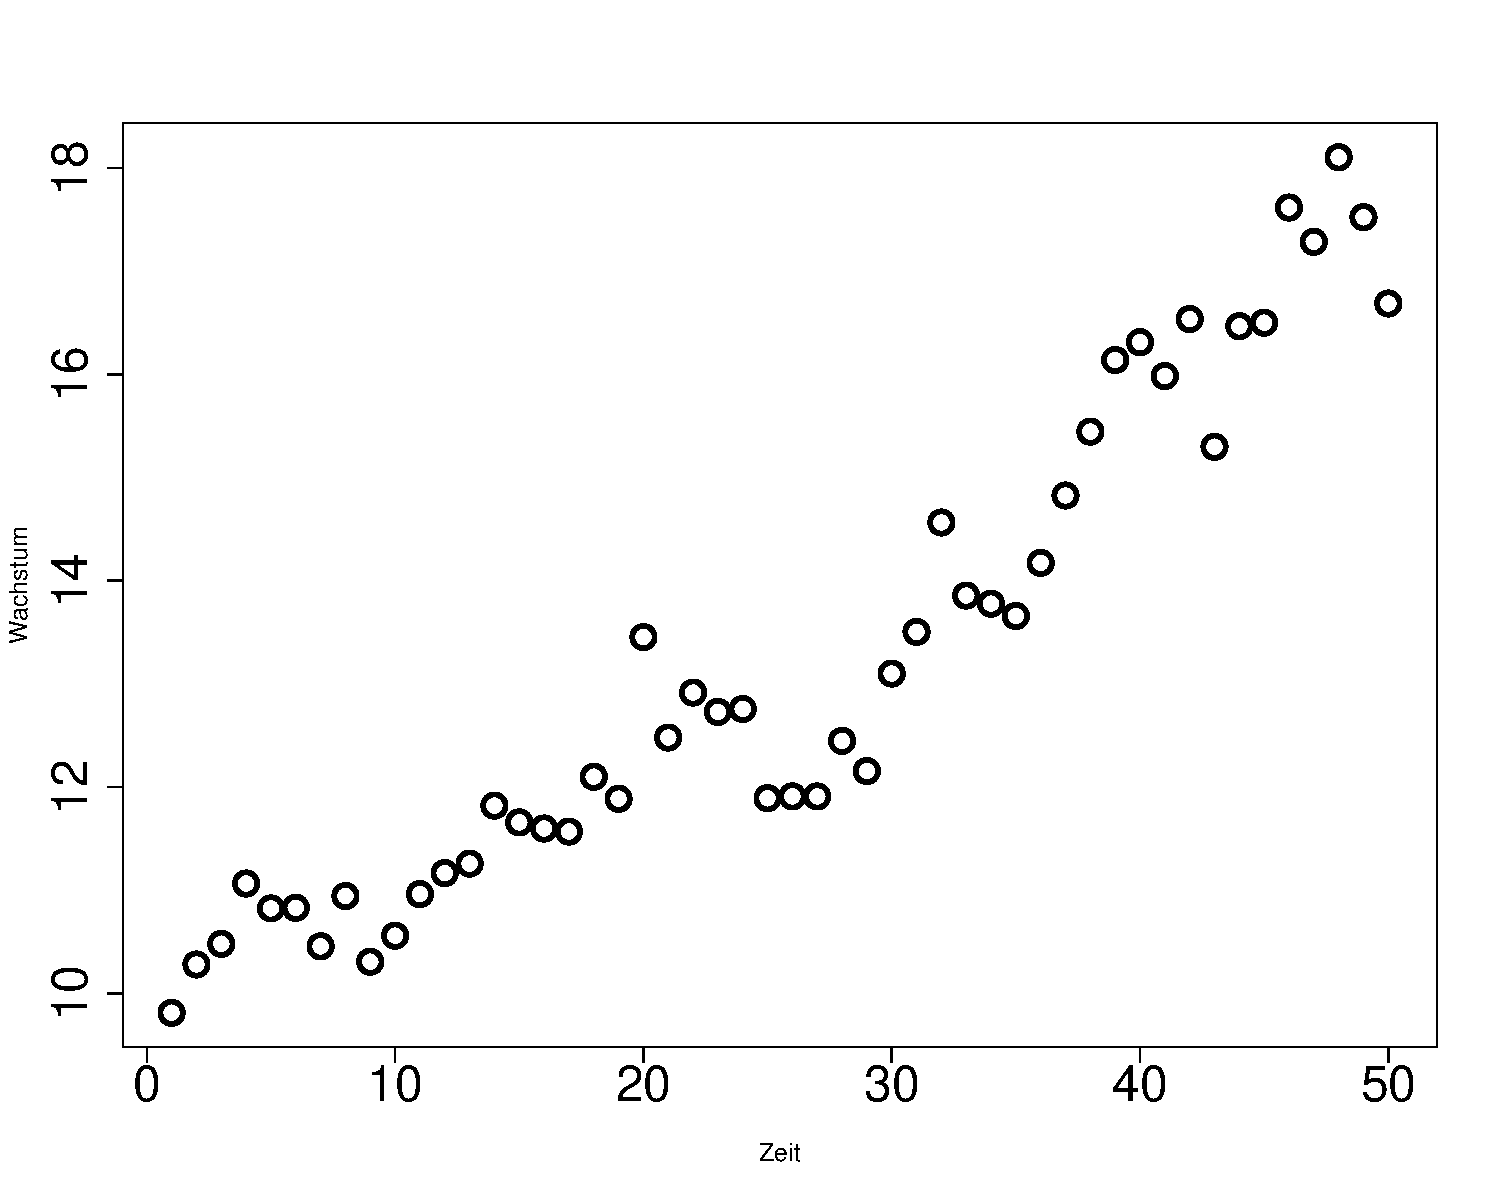
\includegraphics[width=0.5\textwidth]{data-raw}
  \caption{Plot der Beispieldaten}
  \label{Beispieldaten}
\end{figure}

In den folgenden Kapiteln wird mit einem normierten $Y$ gearbeitet, indem durch $\max(Y)$ geteilt wird. Dadurch erhält man Werte zwischen Null und Eins, wodurch sich die Berechnungen vereinfachen.

Man kann dies machen, da von 

\begin{equation*}
Y=X\beta+e
\end{equation*}

ausgehend, man zu 

\begin{equation*}
\max(Y)^{-1} Y = X \max(Y)^{-1} \beta + \max(Y)^{-1} e =: X \tilde{\beta} + \tilde{e}
\end{equation*}

gelangt und dieses Modell immer noch multiple linear und homoskedastisch ist. 

Man kann ohne Einschränkung der Allgemeinheit davon ausgehen, dass die Elemente von $X$ Werte in $[0,1]$ annehmen. Sind die Werte nicht in $[0,1]$ kann man mit $\max(X)$ normieren.

Insgesamt erhält man aus $\tilde{\beta}$ wieder $\beta$ indem man mit $\max(Y)$ multipliziert.  

Benutzt man die Formeln \eqref{beta} und \eqref{sigma} von oben erhält man  $\hat{\beta}$=\betaoneest und $\widehat{\sigma^2}$=\sigmaoneest. In folgender Graphik \ref{Beispieldaten_Regressionsgerade} sind die Daten mit der Regressionsgerade eingezeichnet.

\begin{figure}[H] 
  \centering
     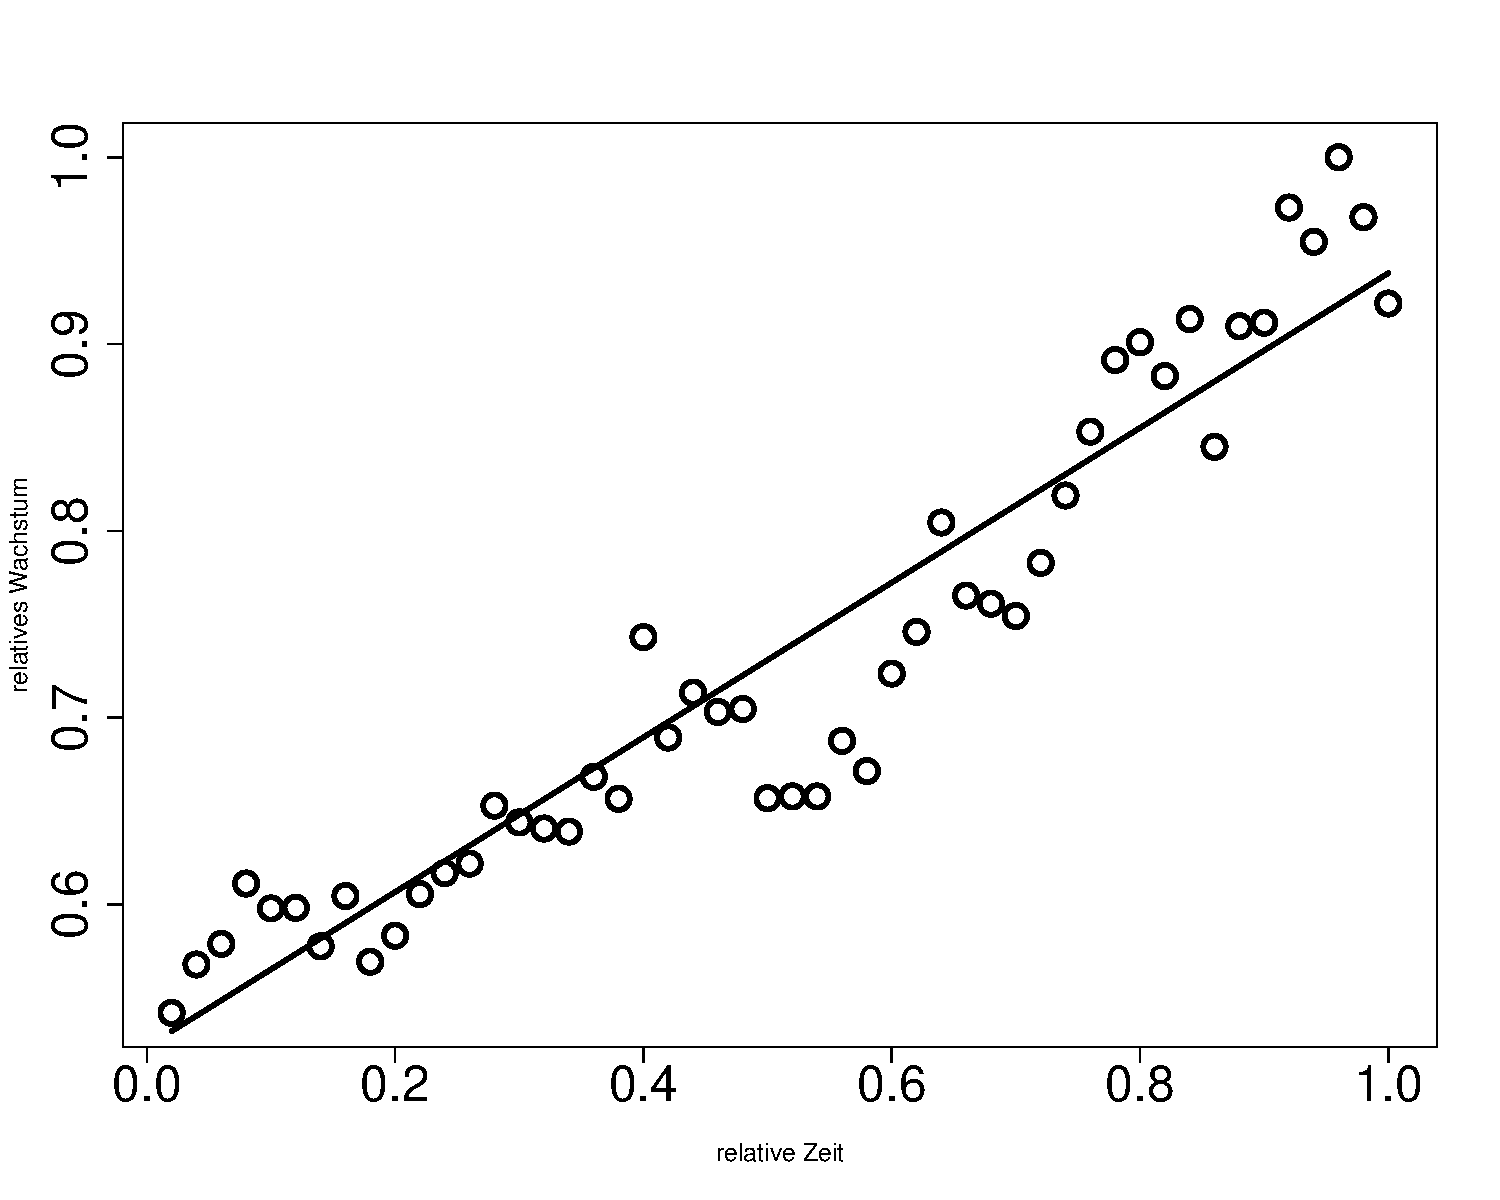
\includegraphics[width=0.5\textwidth]{regression-gerade}
  \caption{Plot der Beispieldaten mit Regressionsgerade}
  \label{Beispieldaten_Regressionsgerade}
\end{figure}
 
\end{Beispiel} 



\subsection{Konfidenzbänder}
\label{Konfidenzbaender}
In diesem Abschnitt werden Konfidenzbänder definiert und der Unterschied zwischen punktweisen und gleichmäßigen Konfidenzbändern wird erklärt. Die folgende Definition orientiert sich an \cite[229]{Georgii09}.

\begin{Definition}
Sei $( \chi, \mathscr{F} , \mathbb{P}_\vartheta : \vartheta \in \Theta) $ ein stochastisches Modell, $\Sigma$ eine beliebige Menge, $\tau : \Theta \rightarrow \Sigma $ eine zu ermittelnde Kenngröße für den Parameter, und $0 < \alpha < 1$. Dabei bezeichnet \gls{P(...)} ein Wahrscheinlichkeitsmaß.

Eine Abbildung $C : \chi \rightarrow \mathscr{P}(\Sigma)$, die jedem möglichen Beobachtungsergebnis $x \in \chi$ eine Menge $C(x) \subset \Sigma$ zuordnet, heißt ein Konfidenz- oder Vertrauensbereich für $\tau$ zum Irrtumsniveau \gls{Wkeit} (beziehungsweise Sicherheitsniveau 1 - $\alpha$), wenn

\begin{equation*}
\inf_{\vartheta \in \Theta} \mathbb{P}_{\vartheta}(x \in \chi : C(x) \ni \tau(\vartheta)) \geq 1 - \alpha.
\end{equation*}

\end{Definition}

In dieser Ausarbeitung wird immer davon ausgegangen, dass $C(x)$ von der Form $C(x) = \{ y \in \mathbb{R}^n :  x'\hat{\beta} - c ~ \hat{\sigma}\sqrt{x'(X'X)^{-1}x} \leq y \leq x'\hat{\beta} + c ~ \hat{\sigma}\sqrt{x'(X'X)^{-1}x} \}$ ist. Dabei ist $c$ der sogenannte  \gls{kritischer-Wert}.
 
Für den Rest der Ausarbeitung wird dies durch

\begin{equation*}
\mathbb{P}(x' \beta \in x'\hat{\beta} \pm c ~ \hat{\sigma}\sqrt{x'(X'X)^{-1}x}) = 1 - \alpha
\end{equation*} 

abgekürzt. Eine andere mögliche Schreibweise ist 

\begin{equation*}
\mathbb{P}(x'\beta \in M_n(x;Y,\alpha)) = x - \alpha
\end{equation*}

mit 

\begin{equation*}
M_n(x) = (x'\hat{\beta} -c, x'\hat{\beta} +c) 
\end{equation*}

und $c$ passend.

Weiterhin unterscheidet man punktweise und gleichmäßige Konfidenzbänder. Für punktweise Konfidenzbänder gilt für alle $x=(x_{1}, \ldots x_{p}) \in \mathbb{R}^{p+1}$

\begin{equation*}
\mathbb{P}(x'\beta \in x' \hat{\beta} \pm c) = 1-\alpha
\end{equation*}

während für gleichmäßige 

\begin{equation*}
\mathbb{P}(x'\beta \in x' \hat{\beta} \pm c ~ \text{ für alle } x \in \mathbb{R}^{p+1}) = 1-\alpha
\end{equation*}

gilt. Dabei ist $\beta=(\beta_{0}, \ldots, \beta_{p})$ der Koeffizientenvektor, der das Modell festlegt, $\hat{\beta}$ ein Schätzer für $\beta$. 

In dieser Ausarbeitung werden nur gleichmäßige Konfidenzbänder betrachten.



%\begin{Beispiel}
%
%In der folgenden Graphik habe ich das Beispiel aus dem vorherigen Absatz um punktweise wie auch simultane Konfidenzbänder erweitert. Das punktweise Konfidenzband habe ich mit \cite[15]{Liu64} bestimmt. Für das gleichmäßige Konfidenzband habe ich die Methode aus dem nächsten Abschnitt verwendet.
%
%\begin{figure}[H] 
%  \centering
%     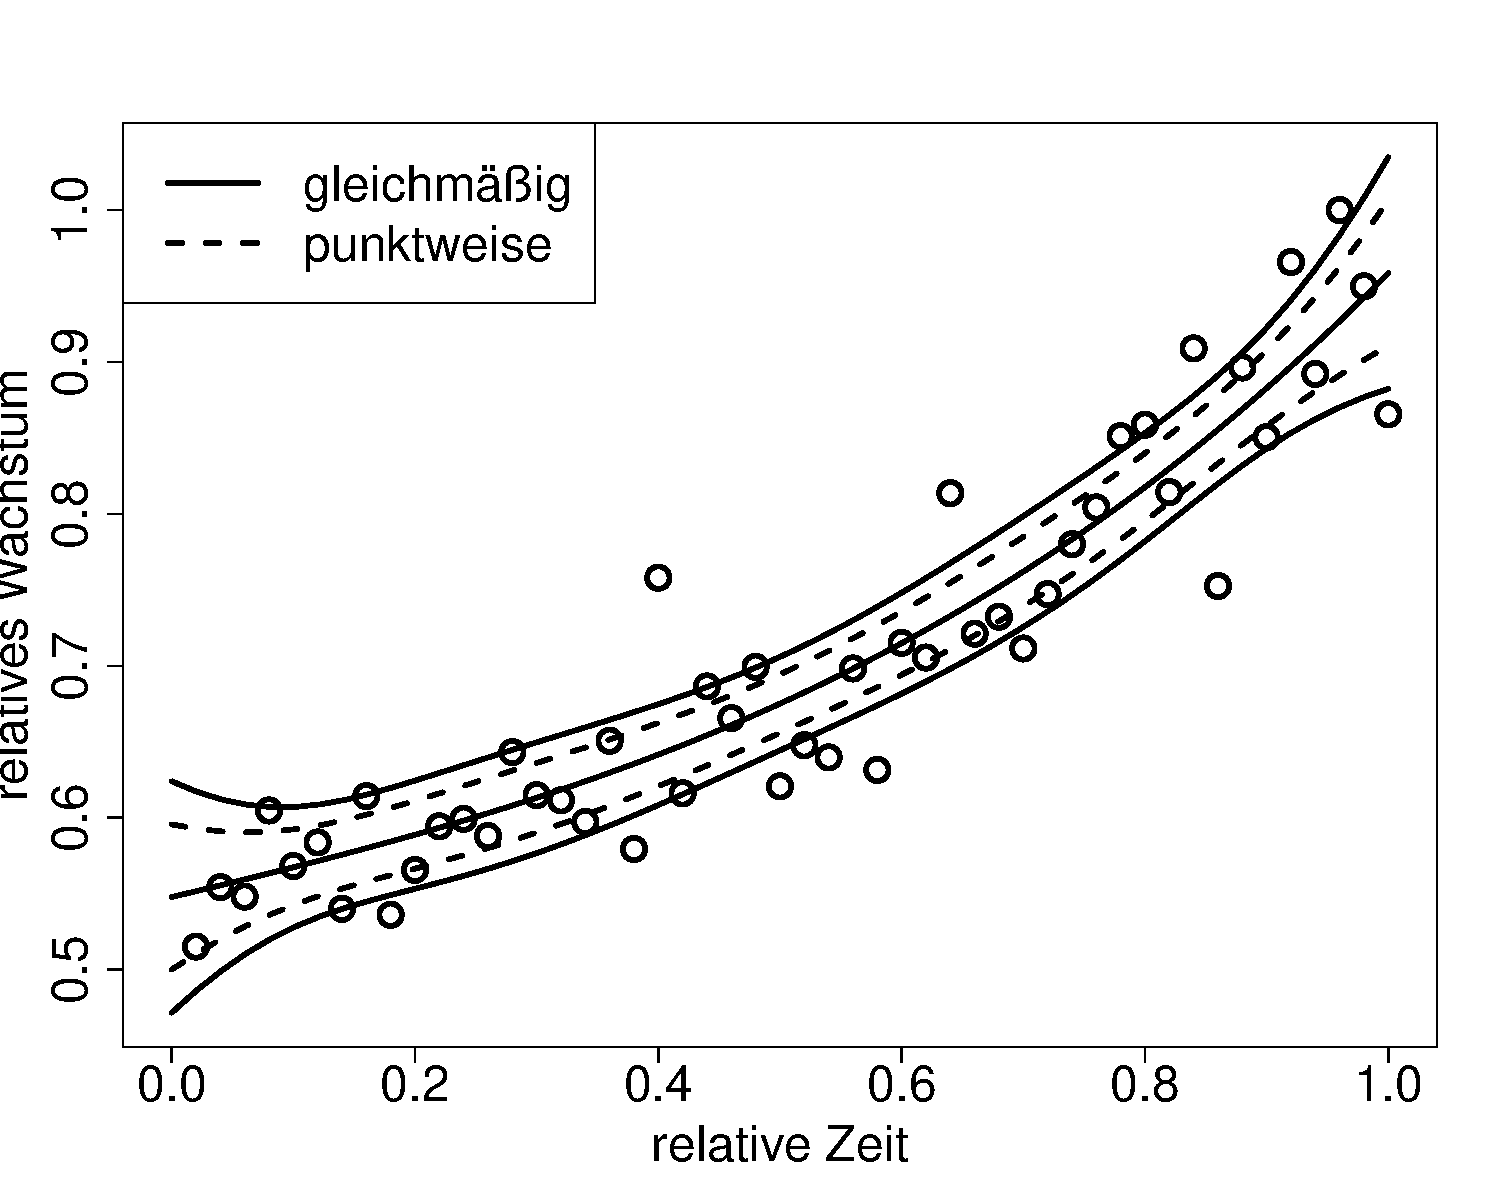
\includegraphics[width=0.5\textwidth]{punkt-vs-gleich}
%  \caption{Vergleich von punktweisen und gleichmäßigen Konfidenzbändern im Beispiel}
%  \label{punkt-vs-gleich_Beispiel}
%\end{figure}
%
%Man sieht, dass das gleichmäßige weiter ist, als das punktweise.
%
%\end{Beispiel}

 

\subsection{Konfidenzbänder auf $\mathbb{R}^{n}$ für ein multiples lineares Regressionsmodell}
\label{Konfidenzbaender auf R fuer ein multiples lineares Regressionsmodell}
Seien  $x,\beta, \hat{\beta}  \in \mathbb{R}^{p+1}$, $X \in \mathbb{R}^{n \times (p+1)}$. In dem verbleibenden Teil dieses Kapitels werden Konfidenzbänder der Form

\begin{equation*} \label{KB_allgemein}
x' \beta \in x'\hat{\beta} \pm c ~ \hat{\sigma}\sqrt{x'(X'X)^{-1}x}
\end{equation*}

bestimmt. Dabei wird der kritische Parameter $c$ so gewählt, dass 

\begin{equation*}
\mathbb{P}(x' \beta \in x'\hat{\beta} \pm c \hat{\sigma}\sqrt{x'(X'X)^{-1}x} ~ \text{ für alle } x \in A)=1-\alpha
\end{equation*}

gilt. Dabei ist $A$ ein Bereich, dem aus bestimmten Gründen besonders interessiert gilt. Mehr zur Wahl von $A$ steht im nächsten Abschnitt. In diesem Abschnitt ist $A = \mathbb{R}^n$.

Wegen des folgenden Resultates aus \cite[66]{Liu64} benutzten wir diese Form von Konfidenzbändern.

\begin{Satz} \label{KB_Eigenschaft}
Für beliebiges $\beta \in \mathbb{R}^{p+1}$ und $\sigma > 0$ gilt 
\begin{equation*}
\mathbb{P}( x'\beta \in x' \hat{\beta} \pm \sqrt{(p+1) f^{\alpha}_{p+1,n-p-1}} \hat{\sigma} \sqrt{x' (X'X)^{-1}x} ~ \text{ für alle } x \in \mathbb{R}^p) = 1 - \alpha
\end{equation*}
\end{Satz} 

Dabei ist \gls{f} das $\alpha$-Quantil der F-Verteilung mit Parametern $p+1$ und $n-p-1$. Dieser Satz eröffnet uns eine einfache Möglichkeit, Konfidenzbänder auf $\mathbb{R}^n$ zu bestimmen. Da das Konfidenzband in Satz \ref{KB_Eigenschaft} von hyperbolischer Form ist, betrachteten wir in den folgenden Abschnitten immer hyperbolische Konfidenzbänder.

Um den Satz \ref{KB_Eigenschaft} beweisen zu können, brauchen wir die folgenden Resultate:

\begin{Lemma} \label{Basiseigenschaft}
Es ist
\begin{eqnarray*}
&&\mathbb{P}( x'\beta \in x' \hat{\beta} \pm c ~ \hat{\sigma} \sqrt{x' (X'X)^{-1} x} ~ \text{ für alle } x \in A ) \\
&=& \mathbb{P}( \sup_{a<x<b} \bigg \vert \frac{x'(\beta - \hat{\beta})}{\hat{\sigma} \sqrt{x'(X'X)^{-1}x}} \bigg \vert \leq c) \\
&=& \mathbb{P}( S \leq c)
\end{eqnarray*}
mit 

\begin{equation*}
\sup_{a<x<b} \frac{\vert x'(\beta - \hat{\beta}) \vert}{\hat{\sigma} \sqrt{x'(X'X)^{-1}x}}  =:  \gls{S}
\end{equation*}

\end{Lemma}

\begin{proof}
\begin{eqnarray*}
&& \mathbb{P}( x'\beta \in x' \hat{\beta} \pm c \hat{\sigma} \sqrt{x' (X'X)^{-1}x} ~ \text{ für alle } x \in A ) \\
&=& \mathbb{P}( x' \hat{\beta} - c \hat{\sigma} \sqrt{x' (X'X)^{-1}x} \leq x'\beta \leq x' \hat{\beta} + c \hat{\sigma} \sqrt{x' (X'X)^{-1}x} ~ \text{ für alle } x \in A ) \\
&=& \mathbb{P}( - c \hat{\sigma} \sqrt{x' (X'X)^{-1}x} \leq x' (\beta - \hat{\beta}) \leq  c \hat{\sigma} \sqrt{x' (X'X)^{-1}x} ~ \text{ für alle } x \in A ) \\
&=& \mathbb{P}( - c  \leq \frac{x' (\beta - \hat{\beta})}{\hat{\sigma} \sqrt{x' (X'X)^{-1}x}}  \leq  c ~ \text{ für alle } x \in A ) \\
&=& \mathbb{P}( \sup_{a<x<b}  \frac{\vert x'(\beta - \hat{\beta}) \vert}{\hat{\sigma} \sqrt{x'(X'X)^{-1}x}}  \leq c)
\end{eqnarray*}
\end{proof}

Es geht in den folgenden Abschnitten immer darum, die Verteilung von $S$ zu bestimmen. Um diese Verteilung auf ganz $\mathbb{R}^n$ zu bestimmen, wird das folgende Ergebnis benutzt, welches sich an \cite[6]{Liu64} orientiert. 

\begin{Satz} \label{Basiseigenschaften}
Wenn das Modell \eqref{Grundmodell_Regression} homoskedastisch ist, gilt nach Satz \ref{erster Satz} 

\begin{enumerate}
\item $\hat{\beta} \sim \mathscr{N}_{p+1}(\beta,\sigma^2(X'X)^{-1})$. Dabei ist $\mathscr{N}_{p+1}(\beta,\sigma^2(X'X)^{-1})$ die ($p$+1)-dimensionale Normalverteilung mit Erwartungswert $\beta$ und Kovarianzmatrix $\sigma^2 (X'X)^{-1}$.
\item $\hat{e} \sim \mathscr{N}_n(0,\sigma^2(I-H)) $ mit  \gls{H} $=X(X'X)^{-1}X' $
\item $\hat{\sigma}^2 \sim \frac{\sigma^2}{n-p-1}\chi_{n-p-1}^2 = \frac{\sigma^2}{v}\chi^2_{n-p-1}$. Dabei ist $n-p-1 :=$ \gls{v}, was ich auch in Zukunft so beibehalten werde. Weiterhin ist \gls{chi-square} die Chi-Quadrat-Verteilung.
\item $\hat{\beta}$ und $\widehat{\sigma^2}$ sind unabhängig.
\end{enumerate}
\end{Satz}

\begin{proof}
1. 
Benutzt man Modell \eqref{Grundmodell_Regression} und die Voraussetzung $ e \sim \mathscr{N}_0,\sigma^2)$ so ist $Y=X \beta + e \sim \mathscr{N}_{n}(X\beta,\sigma^2 I)$. Da aus \eqref{beta} folgt, dass $\hat{\beta} = (X'X)^{-1} X' Y$ gilt, ist $\hat{\beta}$ eine Linearkombination von $Y$. Daraus folgt, dass auch $\hat{\beta}$ normalverteilt ist. Es reicht den Erwartungswert und die Kovarianz zu bestimmen. 

\begin{align*}
E(\hat{\beta}) = E((X'X)^{-1}X'Y) = (X'X)^{-1} X' E(Y) = (X'X)^{-1} X'X \beta = \beta
\end{align*}

und

\begin{eqnarray*}
\text{Cov}(\hat{\beta}) &=& \text{Cov}((X'X)^{-1} X' Y) = ((X'X)^{-1}X') \text{Cov}(Y) (X(X'X)^{-1}) \\
&=& ((X'X)^{-1}X') \sigma^2 I (X(X'X)^{-1}) = \sigma^2 (X'X)^{-1}
\end{eqnarray*}


2.
Da nach \eqref{e} gilt, dass $\hat{e}=(I-H)Y$, ist $\hat{e}$ auch eine Linearkombination von Elementen aus $Y$. Da $Y$ normalverteilt ist, ist es also auch $\hat{e}$. Berechnet man wieder Erwartungswert und Kovarianz, erhält man:

\begin{eqnarray*}
E(\hat{e}) &=& E((I-H)Y) = (I-H)E(Y) = (I-H)X\beta \\ 
&=& (I-X(X'X)^{-1}X')X = X-X(X'X)^{-1}X'X = X-X = 0
\end{eqnarray*}

und

\begin{align*}
\text{Cov}(\hat{e}) = \text{Cov}((I-H)Y) = (I-H) \text{Cov}(Y) (I-H) = \sigma^2 (I-H)
\end{align*}

Bei dieser Berechnung wird benutzt, dass die Matrix $I-H$ sowohl symmetrisch als auch idempotent ist. 

Die Matrix $I-H$ ist symmetrisch, da $H=X'(X'X)^{-1}X$ symmetrisch ist. Weiterhin ist die Matrix idempotent, da

\begin{eqnarray*}
(I-H)^2 &=& (I-X(X'X)^{-1}X')(I-X(X'X)^{-1}X') \\
&=& I + X(X'X)^{-1} X'X(X'X)^{-1}X' - 2 X(X'X)^{-1}X' \\
&=& I - X(X'X)^{-1}X' - X(X'X)^{-1}X'+ x(X'X)^{-1}X' \\
&=& (I-H)
\end{eqnarray*}

3. 
Sei $Q=I-H$ mit $H = X (X'X)^{-1} X'$, dann ist $Q$ symmetrisch und idempotent. Daraus folgt

\begin{eqnarray*}
\text{Rang}(Q) &=& \text{Spur}(Q) = \text{Spur}(I) - \text{Spur}(H) \\
		&=& n - \text{Spur}(X(X'X)^{-1}X') = n - \text{Spur}((X'X)^{-1}X'X) \\
		&=& n - (p+1)
\end{eqnarray*}

Dabei benutzt man $\text{Spur}(AB) = \text{Spur}(BA)$ . 

Also kann man $Q$ ausdrücken als $ Q = T' L T$. Dabei ist $T$ eine orthogonale Matrix und $L$ eine passende Diagonalmatrix mit den ersten $n-(p+1)$ Diagonalelementen Eins und den verbleibenden Diagonalelementen gleich Null.

Es ist $e=Y-X\beta \sim \mathscr{N}_n(0,\sigma^2I)$. Sei $z=Te$ mit $z\sim \mathscr{N}_n(0,\sigma^2I)$. Solch ein $T$ existiert, da $T$ orthogonal ist. 

Weiterhin ist 

\begin{eqnarray*}
Qe = (I-H) (Y-X\beta) = (I-H)Y - (I-H)X \beta = (I-H)Y = \hat{e}
\end{eqnarray*}

da $(I-H)X=0$, wie oben bereits berechnet. Es folgt

\begin{eqnarray*}
\Vert \hat{e} \Vert^2 &=& \Vert Qe \Vert^2 = e'Q'Qe = e'Qe = (Te)' L (Te) \\
&=& z_1^2 + \ldots + z_{n-p-1}^2 \sim \sigma^2 \chi_{n-p-1}^2
\end{eqnarray*}

Setzt man dies nun in Gleichung \eqref{sigma}, das heißt $ \hat{\sigma}^2 = \Vert \hat{e} \Vert^{2} / (n-p-1) $, ein, erhält man 
\[
\hat{\sigma}^2 = \Vert \hat{e} \Vert^{2} / (n-p-1) \sim \frac{\sigma^2}{n-p-1} \chi_{n-p-1}^2
\]

4. Da $\hat{\beta}$ und $\hat{e}$ normalverteilt sind, reicht es für die Behauptung der Unabhängigkeit zu zeigen, dass die Kovarianz zwischen den Beiden Null ist.

\begin{eqnarray*}
\text{Cov}(\hat{\beta},\hat{e}) &=& \text{Cov}((X'X)^{-1} X' Y, (I-H)Y) \\
&=& (X'X)^{-1} X' \text{Cov}(Y,Y) (I-H) \\
&=& \sigma^2 (X'X)^{-1} X' (I-H) = 0
\end{eqnarray*}

\end{proof}

Da wir nun von allen Bausteinen von $S$ die Verteilung kennen, können wir den Satz \ref{KB_Eigenschaft} beweisen. Satz und Beweis orientiert sich an \cite[66]{Liu64}.

\begin{proof}
Zu zeigen war, dass für beliebiges $\beta \in \mathbb{R}$ und $\sigma > 0$  im homoskedastischen Fall

\begin{equation*}
\mathbb{P}( x'\beta \in x' \hat{\beta} \pm \sqrt{(p+1) f^{\alpha}_{p+1,n-p-1}} \hat{\sigma} \sqrt{x' (X'X)^{-1}x}) ~ \text{ für alle } x \in \mathbb{R}^{n}) = 1 - \alpha
\end{equation*}

gilt. 

Sei \gls{P} die eindeutige Wurzel aus $(X'X)^{-1}$ und somit $(X'X)^{-1} = P^2$. Weiterhin definiere \gls{N}=$P^{-1}(\hat{\beta}-\beta)/\sigma$. Dann hat $N$ eine multivariate Normalverteilung $\mathscr{N}_{p+1}(0,I)$ . 

Damit gilt
\begin{eqnarray*}
&&\mathbb{P}(x'\beta \in \sqrt{(p+1) f^{\alpha}_{p+1,n-p-1}} \hat{\sigma} \sqrt{x'(X'X)^{-1}x} ~ \text{ für alle } x \in \mathbb{R}) \\ 
&=& \mathbb{P} \big ( \sup_{x \in \mathbb{R}} \frac{|x'(\hat{\beta}-\beta)|}{\hat{\sigma} \sqrt{x'(X'X)^{-1}x}} \leq \sqrt{(p+1) f^{\alpha}_{p+1,n-p-1}} \big ) \\
&=& \mathbb{P} \big ( \sup_{x \in \mathbb{R}} \frac{|(Px)'N|}{(\hat{\sigma}/\sigma)\sqrt{(Px)'(Px)}} \leq \sqrt{(p+1) f^{\alpha}_{p+1,n-p-1}} \big ) \\
&=& \mathbb{P} \big ( \frac{\parallel N \parallel}{(\hat{\sigma}/\sigma)} \bigg ( \sup_{x \in \mathbb{R}} \frac{|(Px)'N|}{||Px|| ||N||} \bigg ) \leq \sqrt{(p+1) f^{\alpha}_{p+1,n-p-1}} \big ) \\
&=& \mathbb{P} \big (\frac{\parallel N \parallel}{(\hat{\sigma}/\sigma)} \leq \sqrt{(p+1) f^{\alpha}_{p+1,n-p-1}} \big ) \\
&=& \mathbb{P} \big (\frac{(\hat{\beta}-\beta)'(X'X)(\hat{\beta}-\beta)}{(p+1)\hat{\sigma}^2} \leq f^{\alpha}_{p+1,n-p-1} \big ) \\
&=& 1 - \alpha
\end{eqnarray*}

Dabei wird im vorletzten Schritt  die Cauchy-Schwarz-Ungleichung $ \vert (Px)'N \vert \leq \Vert Px \Vert \Vert N \Vert $ verwendet. Gleichheit gilt, falls $P x = \lambda N$ für ein $N$ . 

Im letzten Schritt wird aus Satz \ref{Basiseigenschaften} benutzt, dass sowohl $(\hat{\beta}-\beta)'(X'X)(\hat{\beta}-\beta)$ als auch $(p+1)\hat{\sigma}^2$ $\chi^2$-verteilt sind. Außerdem sind beide unabhängig und somit ist ihr Quotient F-verteilt.

\end{proof}

\begin{Beispiel}
In der folgenden Abbildung \ref{KB-ganz-R-BSP} sind die Daten aus dem letzten Beispiel wieder mit einer polynomiellen Regression vom Grad Eins eingezeichnet.

Diesmal wird dazu noch ein Konfidenzband auf ganz $\mathbb{R}$ eingezeichnet. Die Berechnung ist in der Datei \textit{beispiele.R} im Ordner \textit{5-Beispiele} zu finden. Als kritischen Parameter für das Konfidenzband hat sich \cR . ergeben.

\begin{figure}[H] 
  \centering
     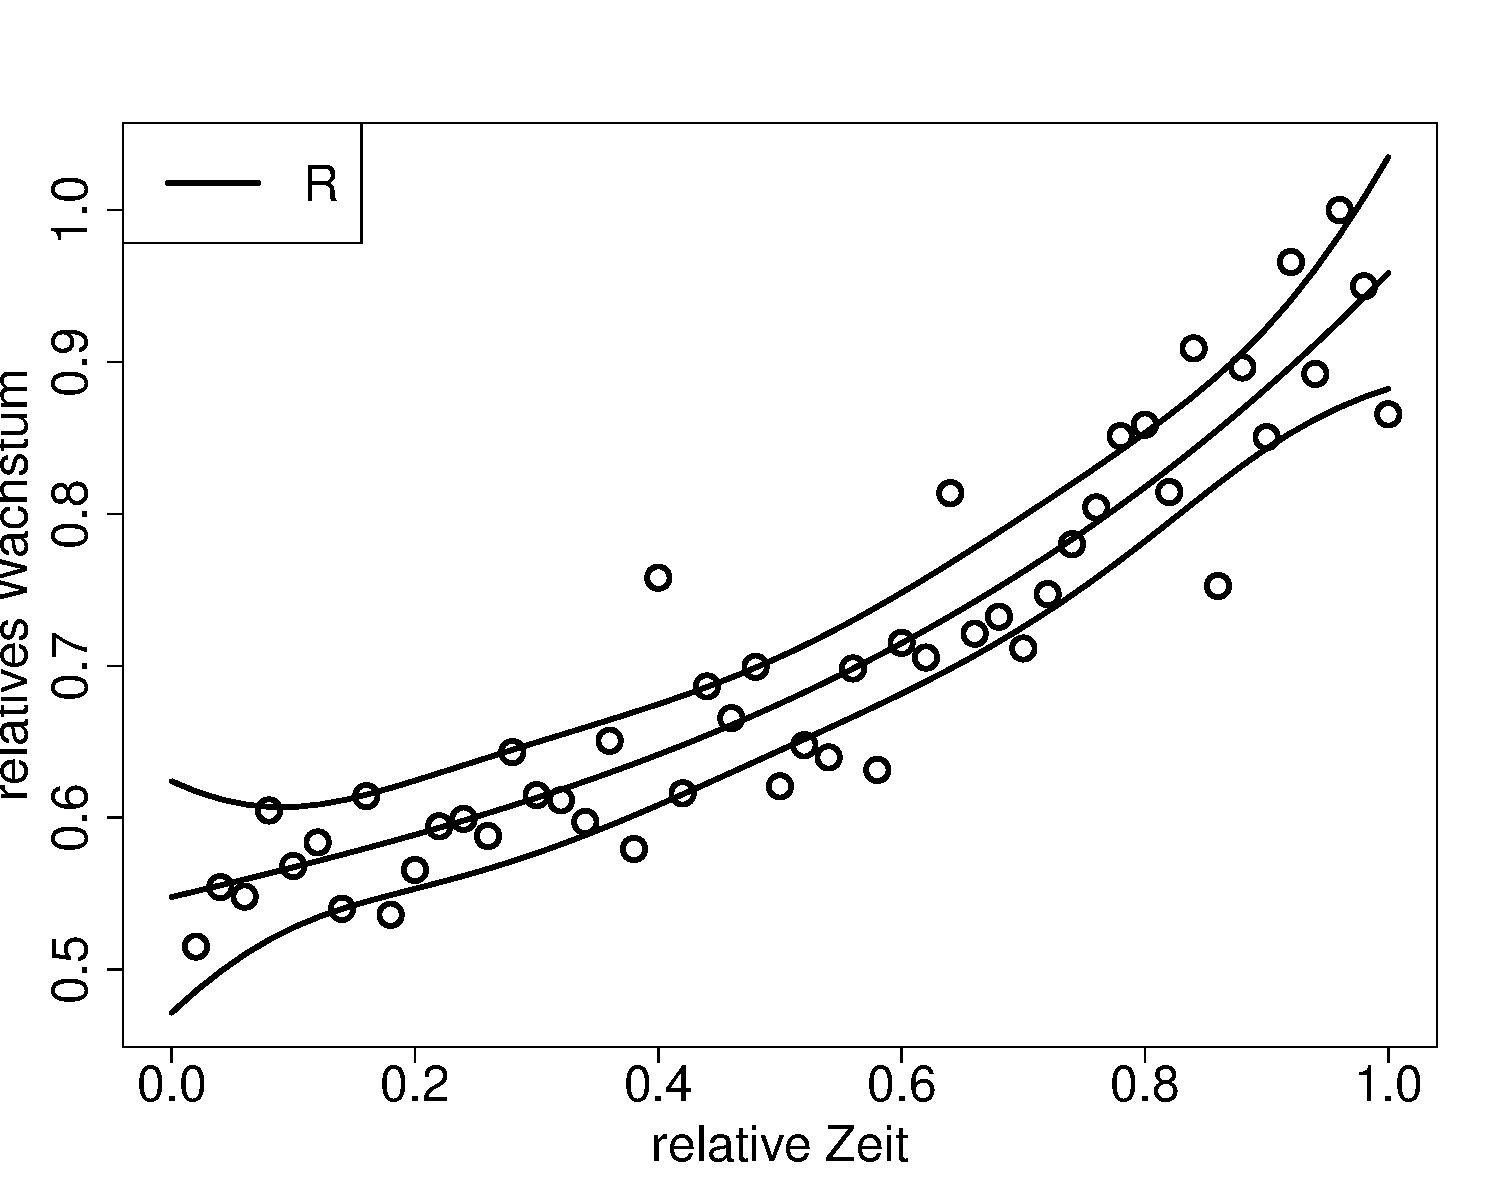
\includegraphics[width=0.5\textwidth]{Bsp-KB-R}
  \caption{Weiterführung des Beispiels durch Konfidenzband auf ganz $\mathbb{R}$}
  \label{KB-ganz-R-BSP}
\end{figure}

\end{Beispiel}

\begin{Simulation}
Als nächstes wird eine Simulation durchgeführt, um die Überdeckungswahrscheinlichkeit der Methoden zu überprüfen.

Dazu werden Daten auf zwei verschiedene Arten erzeugt. Zum einen habe lege ich als Grundmodell ein multiples lineares, homoskedastisches Regressionsmodell zugrunde, zum anderen lege ich ein multiples lineares Regressionsmodell mit einem AR(1)-Prozess zugrunde. 

Bei der Simulation erzeuge ich zuerst \ntest mal Daten mit den oben genannten Grundmodellen. Danach erzeuge ich Konfidenzbänder um ein OLS beziehungsweise mit einem AR(1) transformierten OLS-Schätzer. Dann wird gezählt, wie oft das wahre Modell in dem Konfidenzband liegt. 

Die Ergebnisse sind in der folgenden Tabelle zusammengestellt. Die erste Spalte gibt die Überdeckungswahrscheinlichkeit bei dem homoskedastischen Modell an, die zweite bei einem AR(1)-Grundmodell. 

Diese Tabelle wird um weiter Zeilen mit den anderen Methoden Konfidenzbänder zu erzeugen erweitert, nachdem die neuen Methoden eingeführt sind.

\begin{center}
\begin{tabular}{|c|c|c|}
\hline 
$\times$ & R & AR \\ 
\hline 
R & \UeberRR & \UeberARR \\ 
\hline 
\end{tabular}
\end{center}

\end{Simulation}



\subsection{Konfidenzbänder auf einem Intervall für ein einfaches lineares Regressionsmodell}
\label{Konfidenzbänder auf einem Intervall für ein einfaches lineares Regressionsmodell}
Dieser Abschnitt orientiert sich an \cite[17-23]{Liu64} und \cite{Liu08} und \cite{Wynn71}.

Für den Fall, dass wir nur einen unabhängige Variable $x_1$ haben vereinfacht sich das Konfidenzband \ref{KB_allgemein} zu

\begin{equation}\label{simple_KB}
\mathbb{P}(\beta_0 + \beta_1 x_1 \in \hat{\beta_0} + \hat{\beta_1} x \pm c \hat{\sigma} \sqrt{\nu(1,x_1)}  \text{ für alle } x \in (a,b) )
\end{equation}

Dabei und für diesen Abschnitt gelten die folgenden Definitionen

\begin{eqnarray*}
P^2 &=& (X'X)^{-1} \\
N &=& P^{-1} (\hat{\beta} - \beta)/\sigma) \sim \mathscr{N}_2(0,I_2) \\
T &=& N / (\hat{\sigma} / \sigma) = P^{-1} (\hat{\beta}-\beta) / \hat{\sigma} \\
v &=& n-2 \\
x_1 &=& x \\
\nu(c,d) &=& (c,d) (X'X)^{-1} (c,d)' \\
A &=&(a,b)
\end{eqnarray*}

Aus \cite[19-20]{Liu64} hat man folgende Ergebnisse

\begin{eqnarray*}
\mathbb{P}(\beta_0 + \beta_1 x \in \hat{\beta_0} + \hat{\beta_1} x \pm c \hat{\sigma} \sqrt{\nu(1,x)}  \text{ für alle } x \in (a,b)  \\
= \mathbb{P} (\sup_{x \in (a,b)} \vert (1,x) ( \hat{\beta} - \beta ) / \hat{\sigma} \vert / \sqrt{\nu(1,x)} < c) \\
= \mathbb{P} (\sup_{x \in (a,b)} \vert (P \cdot (1,x)')' \cdot T \vert / \Vert P \cdot (1,x)' \Vert < c) \\
= \mathbb{P} (T \in R_{h,2})
\end{eqnarray*}

dabei ist

\begin{equation*}
R_{h,2}(x) = ( T : \vert (P \cdot (1,x)' )' \cdot T \vert / \Vert P \cdot (1,x)' \Vert < c)
\end{equation*}

ein Region von der Form $(T : \vert v'T \vert / \Vert v \Vert < r) \subset \mathbb{R}^2$. Deswegen kann man den Winkel $\phi$ zwischen den Vektoren $P \cdot (1,a)'$ und $P \cdot (1,b)'$ mittels

\begin{eqnarray*}
\cos \phi &=& (P \cdot (1,a)')' (P \cdot (1,b)') / \Vert P \cdot (1,a)' \Vert \Vert P \cdot (1,b)' \Vert \\
&=& (1,a) (X'X)^{-1} (1,b)' / \sqrt{\nu(1,a) \nu(1,b)} 
\end{eqnarray*}

berechnen. Jetzt folgt mit \cite{Wynn71}, dass gilt
%
%\begin{equation*}
%\mathbb{P}( \Vert T \Vert < c ) = \mathbb{P}(R_T < c) = 1 - (1+c^2/\nu)^{-\nu/2}
%\end{equation*}
%
%außerdem hat man
%
%\begin{eqnarray*}
%\frac{2}{\pi} \int^{(\pi-\phi)/2}_{0} \biggl( \bigl( 1 + \frac{c^2}{\nu} \bigr)^{-\nu/2} - \bigl( 1 + \frac{c^2}{\nu \sin^2(\phi + \phi/2)} \bigr)^{-\nu/2} \biggr) \text{d} \phi
%\end{eqnarray*}


\begin{eqnarray*}
\mathbb{P}(\beta_0 + \beta_1 x \in \hat{\beta_0} + \hat{\beta_1} x \pm c \hat{\sigma} \sqrt{\nu(1,x)} \text{ für alle } x \in (a,b) ) \\
= 1 - \frac{\phi}{\pi} \biggl( 1 + \frac{c^2}{v} \biggr)^{ - v/2} - \frac{2}{\pi} \int^{(\pi - \phi)/2}_{0} \biggl( 1 + \frac{c^2}{v \sin^2(\theta + \phi/2)} \biggr)^{-v/2} \text{d} \theta
\end{eqnarray*}

Man muss also 

\begin{equation*}
1 - \frac{\phi}{\pi} \biggl( 1 + \frac{c^2}{v} \biggr)^{ - v/2} - \frac{2}{\pi} \int^{(\pi - \phi)/2}_{0} \biggl( 1 + \frac{c^2}{v \sin^2(\theta + \phi/2)} \biggr)^{-v/2} \text{d} \theta = 1 - \alpha
\end{equation*}

nach $c$ lösen und kann dann das Konfidenzband \eqref{simple_KB} berechnen. Diese Berechnung wird hier nicht durchgeführt.





\subsection{Konfidenzbänder auf einem Intervall für ein multiples lineares Regressionsmodell}
\label{Konfidenzbaender auf einem Intervall fuer ein multiples lineares Regressionsmodell}
Im Abschnitt \ref{Konfidenzbaender auf R fuer ein multiples lineares Regressionsmodell} wurden Konfidenzbänder auf ganz $\mathbb{R}^p$ konstruiert. Allerdings kann es bei der Verwendung einiger unabhängigen Variablen nicht sinnvoll sein, das Konfidenzband auf ganz $\mathbb{R}^{p}$ zu konstruieren. Ist die unabhängige Variable zum Beispiel ein Gewicht, reicht es, ein Konfidenzband auf $\mathbb{R}_{+}^{p}$ zu konstruieren. Schließlich sind Gewichte immer positiv.

Nachfolgend wird das uns interessierende Gebiet mit $A$ bezeichnet. Dabei ist 

\begin{equation*}
A = \{(x_1, \ldots, x_p)' : a_i \leq x_i \leq b_i, i = 1, \ldots, p \} \subset \mathbb{R}^p \text{ für } - \infty \leq a_i < b_i \leq \infty, i=1, \ldots, p
\end{equation*}

Eine Möglichkeit, ein Konfidenzband auf $A$ zu bestimmen, ist, ein Konfidenzband auf ganz $\mathbb{R}^p$ zu konstruieren und dann den Teil auf $\mathbb{R}^{p} \setminus A$ zu vernachlässigen.

Da dann die Bedingung $\mathbb{P}(x'\beta \in x' \hat{\beta} \pm c ~ \text{ für alle } x) = 1-\alpha$ für mehr $x$-Werte als nötig erfüllt sein muss, ist das Konfidenzband dann weiter, als es müsste.

Besser ist die folgende Möglichkeit, die sich an \cite[70]{Liu64} orientiert. Das Ziel ist wieder ein hyperbolisches Konfidenzband der Form 

\begin{equation}
x'\beta \in x' \hat{\beta} \pm c ~ \hat{\sigma} \sqrt{x' (X'X)^{-1}x} \label{hyperbolisches_KB}
\end{equation}

erzeugen, um es mit dem Band aus dem vorherigen Absatz vergleichen zu können. Das Problem ist, ein geeignetes $c$ zu finden, sodass $\mathbb{P}( x'\beta \in x' \hat{\beta} \pm c ~ \hat{\sigma} \sqrt{x' (X'X)^{-1}x} ~ \text{ für alle } x \in A) = 1-\alpha$ gilt.

Es ist aus Satz \ref{Basiseigenschaft} aus dem vorherigen Abschnitt bekannt, dass 

\begin{equation*}
\mathbb{P}( x'\beta \in x' \hat{\beta} \pm c ~ \hat{\sigma} \sqrt{x' (X'X)^{-1}x} ~ \text{ für alle } x \in A ) = \mathbb{P}(S<c)
\end{equation*}

Dabei ist $S$ gegeben durch 

\begin{equation*}
S = \sup_{a<x<b} \frac{\vert x'(\beta - \hat{\beta}) \vert}{\hat{\sigma} \sqrt{x'(X'X)^{-1}x}}
\end{equation*}

Da $S$ nicht von $\beta$ und $\sigma^2$ abhängt, ist es in dieser Hinsicht ein Pivotelement. Dabei ist $\beta$ wieder der Koeffizientenvektor und $\sigma^2$ die Varianz der Fehler. 

Allerdings hängt es immer noch in komplizierter Art und Weise von der Designmatrix $X$ und den Grenzen $a_i$ und $b_i$ von $A$ für $i=1, \ldots, p$ ab. Dies macht $S$ allgemein sehr schwer zu berechnen.

Seien $P$ und $N$ definiert wie im Beweis zu Satz \ref{KB_Eigenschaft}. Das heißt, 

\begin{eqnarray*}
P^2 &=& (X'X)^{-1} \\
N &=& \frac{P^{-1}(\hat{\beta}-\beta)}{\sigma}
\end{eqnarray*}

Dann hat 

\begin{equation*}
T = \frac{N}{(\hat{\sigma} /\sigma)} = \frac{P^{-1}(\hat{\beta}-\beta)}{\hat{\sigma}}
\end{equation*}

eine so genannte \gls{Tau} Verteilung. Damit kann man $S$ ausdrücken als

\begin{eqnarray*}
S &=& \sup_{x \in A} \frac{\vert(Px)'(P^{-1} (\hat{\beta}-\beta)) / \hat{\sigma} \vert}{\sqrt{(Px)'(Px)}}\\
&=& \sup_{x \in A} \frac{\vert (Px)' T \vert}{\Vert Px \Vert} \\
&=& \sup_{v \in C(P,A)} \frac{\vert v'T \vert}{\Vert v \Vert}
\end{eqnarray*}

mit 

\begin{eqnarray*}
C(P,A) &=& \{ \lambda P x : \lambda \geq 0, x \in A \} \\
&=& \{ \lambda (p_0+x_1 p_1 + \ldots +x_p p_p) : \lambda \geq 0, x_i \in [a_i,b_i] ~ \text{ für alle } i=1,\ldots,p \}
\end{eqnarray*}

wobei $P=(p_0, \ldots, p_p)$. 

Allerdings ist es für ein allgemeines $p \leq 1$ sehr schwierig, eine genaue Formel für die Verteilung von $S$ explizit zu bestimmen, um die kritische Konstante $c$ zu bestimmen \cite[S.70, Z.18]{Liu64}. Deswegen wird eine Simulation benutzt.

Man beachte, dass $C(P,A)$ der Kegel ist, der von den Vektoren $p_0+c_1 p_1 + \ldots + c_p p_p $ aufgespannt wird, wobei $c_i$ entweder $a_i$ oder $b_i$ für $i=1,\ldots,p$ ist. 

Sei \gls{Pi} die Projektion von $t \in \mathbb{R}^{p+1}$ auf den Kegel $C(P,A)$, d.h. $\pi(t,P,A)$ löst $ min_{v \in C(P,A)} \Vert v-t \Vert$. Jetzt folgt mit \cite{Naiman87} Theorem 2.1, dass $S$ die Gleichung

\begin{equation*}
S=\max(\Vert \pi(t,P,A) \Vert, \Vert \pi(-t,P,A) \Vert)
\end{equation*}
 
löst. 

Man kann also die kritische Konstante $c$ mit folgender Simulation finden:

\begin{enumerate}
\item Simuliere $N \sim \mathscr{N}_{p+1}(0,I)$ und $\hat{\sigma}/\sigma\sim\sqrt{\chi_v^2/v}$ mit $v=n-p-1$ und $p$ der Anzahl an unabhängigen Parametern.
\item Berechne $\pi(t,P,A)$ und $\pi(-t,P,A)$ .
\item Berechne $S=\max(\Vert \pi(t,P,A) \Vert, \Vert \pi(-t,P,A) \Vert)$ .
\end{enumerate}

Wiederholt man diese Schritte $R$ mal, so erhält man $S_1, \ldots, S_R$. Dann ist $c$ das $1-\alpha$ Quantil von $S_1, \ldots, S_R$.

Um $\pi(t,P,A)$ und $\pi(-t,P,A)$ zu bestimmen, wird folgendes Verfahren verwendet, das aus \cite[Appendix B]{Liu64} stammt:

Es soll das $v$ in $\mathbb{R}^{p+1}$, das $\Vert v-t \Vert^2$ minimiert, gefunden werden. Dabei soll $v \in C(P,A_{r})$ sein, mit $C(P,A_{r})$ wie oben definiert. 

Da betrachten wir

\begin{equation*}
\Vert v-t \Vert^2 = v'v-2t'v+t't 
\end{equation*}
%= (\frac{1}{2} v'v-t'v+\frac{1}{2} t't) \cdot 2

Man sieht, dass $t't$ unabhängig von $v$ ist. Deshalb muss man es bei der Minimierung von $\Vert v-t \Vert^2$ nicht berücksichtigen.
 
Sei $e_j \in \mathbb{R}^{p+1}$ der $j$-te Einheitsvektor. 

Aus der Definition von $C(P,A_{r})$ ist zu sehen, dass $v \in C(P,A_{r})$ impliziert, dass $v=\lambda P x$ oder gleichwertig $P^{-1}v=\lambda x = (\lambda, \lambda x_1, \ldots , \lambda x_p)'$ für ein $x \in A_{r}$ und $\lambda \geq 0$ gelten muss. Deshalb ist $e_1'P^{-1}v = \lambda \geq 0$ und $a_j \leq e_{j+1}'P^{-1}v/e_1'P^{-1}v = x_j \leq b_j$ für $j = 1, \ldots p$ oder gleichwertig

\begin{eqnarray*}
- e_1' P^{-1} v &\leq & 0 \\
(e_{j+1}' - b_j e_1') P^{-1} v &\leq & 0 \textnormal{ für } j = 1, \ldots, p \\
(a_{j} e_1' - e_{j+1}')P^{-1} v &\leq & 0 \textnormal{ für } j = 1, \ldots, p
\end{eqnarray*}

Diese Beschränkungen kann man zusammenfassen zu 

\begin{equation*}
A v \leq 0
\end{equation*}

wobei $A$ die $(2p+1) \times (p+1)$ Matrix

\[ 
A = 
\begin{bmatrix} (e_2'-b_1 e_1')P^{-1}  \\ 
				(a_1 e_1' - e_2')P^{-1}  \\  
				\ldots						 \\ 
				(e_{p+1}' - b_p e_1') P^{-1}	\\  
				(a_p e_1' - e_{p+1}')P^{-1}  \\
				-e_1'P^{1} 
\end{bmatrix}
\]

ist. Für Minimierungsprobleme dieser Art gibt es ein R-Paket namens \textit{Quadprog} , das ich zur Lösung dieser Minimierungsaufgabe benutzt habe.

\begin{Beispiel}
Jetzt wird das Beispiel aus dem Abschnitt \ref{Konfidenzbaender auf R fuer ein multiples lineares Regressionsmodell} fortgeführt, indem zu der Regression mit Grad Eins und dem Konfidenzband auf ganz $\mathbb{R}^{2}$ noch ein Konfidenzband auf $A$ eingezeichnet wird. Dabei benutzt man $A = \{x \in \mathbb{R}^2 : x_i \in [0,1] \text{ für alle } i=1, 2 \} $. 


\begin{figure}[H] 
  \centering
     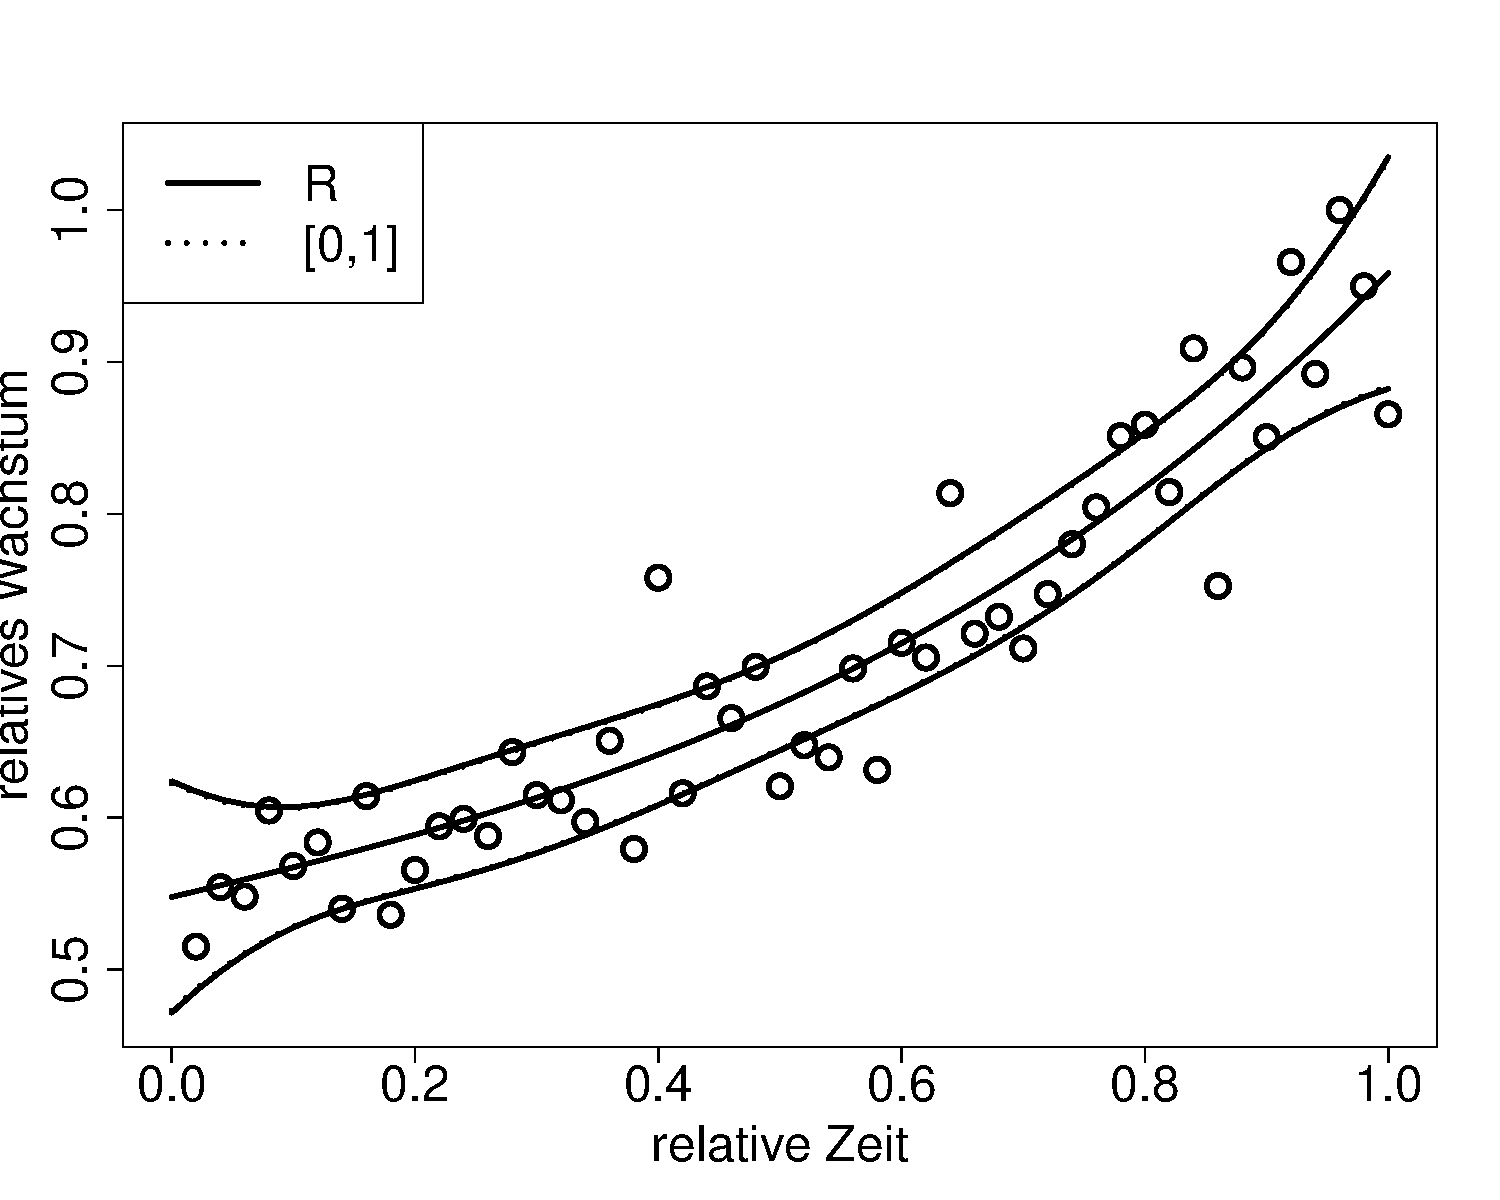
\includegraphics[width=0.5\textwidth]{Bsp-KB-minmax}
  \caption{Weiterführung des Beispiels durch Konfidenzband auf [0,1]}
  \label{KB-minmax-BSP}
\end{figure}

Der kritischen Wert für das Konfidenzband auf ganz $\mathbb{R}^2$, den ich bereits in Abschnitt \ref{Konfidenzbaender auf R fuer ein multiples lineares Regressionsmodell} berechnet hatte war \cR . Für das Konfidenzband auf $A$ ergibt sich \cA . Dieser Wert ist kleiner als der bisherige, was auch zu erwarten war.

Dies sieht man auch daran, dass das Konfidenzband auf $A$ schmaler ist, als das Konfidenzband auf ganz $\mathbb{R}^2$. Der Unterschied wirkt allerdings nicht besonders groß.

Da bei der Berechnung des kritischen Wertes für das Konfidenzband auf $A$ ein Simulation verwendet wird und Reproduktivität gewährleisten sein soll, wird an dieser Stelle die Seed \seedsimulation gesetzt. 

\end{Beispiel}

\begin{Simulation}
Jetzt wird die Simulationstabelle aus dem Abschnitt \ref{Konfidenzbaender auf R fuer ein multiples lineares Regressionsmodell} durch Überdeckungswahrscheinlichkeiten für die Konfidenzbänder auf $A$ fortgesetzt. 

In diesem Fall ist $A = \{x \in \mathbb{R}^2 : x_i \in [0,1] \text{ für alle } i=1, 2 \}$. Dies liegt daran, dass wir die Matrix x so wählen, dass die unabhängigen Variablen im Intervall $[0,1]$ liegen.

\begin{center}
\begin{tabular}{|c|c|c|}
\hline 
$\times$ & R & AR \\ 
\hline 
R 		& \UeberRR & \UeberARR \\ 
\hline 
Minmax 	& \UeberRMinmax & \UeberARMinmax \\ 
\hline 
\end{tabular}
\end{center}

\end{Simulation}



\subsection{Konfidenzbänder auf auf einem Intervall für ein Regressionsmodell mit Polynomgestalt}
\label{Konfidenzbaenderauf auf einem Intervall für Regressionsmodell mit Polynomgestalt}
Betrachten wir nun wieder das Regressionsmodell 

\begin{equation*}
Y=X\beta+e
\end{equation*}

mit $Y$ einem $1 \times n$ Datenvektor, $\beta$ ein $1 \times (p+1)$ Koeffizientenvektor und $e \sim \mathscr{N}_n (0,I_n \sigma^2)$ ein $1 \times n$ Zufallsfehlervektor.

Weiterhin lag in den bisherigen Abschnitten die Annahme zugrunde, dass $X$ irgendeine feste, aber beliebige $n \times (p+1)$ Matrix ist. Diese Annahme nennt man festes Design.

In diesem Abschnitt betrachten wir den Fall, dass die Spalten von $X$ einen funktionalen Zusammenhang erfüllen. Konkret gehen wir davon aus, dass die $i$-te Zeile von $X$ von der Form $\tilde{x}_i = (1,x_i,x_{i}^{2},\ldots,x_{i}^{p})$ hat. 

Unsere Designmatrix ist also zeilenweise von Polynomgestalt. 

Dies ist genau der Fall, den wir in dem Beispiel, das am Ende der Abschnitte steht, betrachtet haben. 

Das Ziel ist es, wieder Konfidenzbänder der Form 

\begin{equation}
x' \beta \in x' \hat{\beta} \pm c \hat{\sigma} \sqrt{x'(X'X)^{-1}x} ~ \text{ für alle } x \in A
\end{equation}

aus den in Abschnitt \ref{Konfidenzbaender auf R fuer ein multiples lineares Regressionsmodell} genannten Gründen zu  finden. 

Dabei ist die kritische Konstante $c$ wieder so zu bestimmen, dass

\begin{equation*}
\mathbb{P}(x' \beta \in x' \hat{\beta} \pm c \hat{\sigma} \sqrt{x'(X'X)^{-1}x} ~ \text{ für alle } x \in A) = 1 - \alpha
\end{equation*}

gilt. 

Es können allerdings nicht direkt die Ergebnisse aus dem letzten Abschnitt benutzen werden. Dies liegt daran, dass es  folgende ungünstige Eigenschaften, die \cite[180]{Liu64} entnommen sind, gibt: 

\begin{enumerate}
\item Angenommen, man versucht die Parameter des Modells $Y=X\beta+e$ zu schätzen, um Konfidenzbänder auf ganz $\mathbb{R}^p$ zu konstruieren. 

Dabei sei $e \sim \mathscr{N}_n(0,\sigma^2 I_n)$ mit bekanntem $\sigma^2$. Das heißt, es ist nur $\beta$ zu Schätzen.

Die beiden Schätzer für $\beta$ seien $\hat{\beta_1}$ und $\hat{\beta_2}$. 

Weiterhin sei $\hat{\beta_1}$ näher an $\beta$ als $\hat{\beta_2}$. Näher meint in diesem Fall, dass

\begin{align*}
\sup_{x \in \mathbb{R}} \frac{\vert x'(\hat{\beta_1} - \hat{\beta}) \vert}{\hat{\sigma} \sqrt{x'(X'X)^{-1}x}} < 
\sup_{x \in \mathbb{R}} \frac{\vert x'(\hat{\beta_2} - \hat{\beta}) \vert}{\hat{\sigma} \sqrt{x'(X'X)^{-1}x}}
\end{align*}

Zu erwarten ist, dass das erste Modell sinnvoll ist, wenn auch das zweite sinnvoll ist. Immerhin ist das erste Modell näher an dem wahren Modell, als das zweite.

Dies ist allerdings für die bisher betrachteten Konfidenzbänder nicht der Fall, da die bisher betrachteten Verfahren die spezielle polynomiale Struktur nicht berücksichtigen. 

\item Die kritische Konstante $c$ kann kleiner als im letzten Abschnitt gewählt werden. Dies liegt daran, dass das Konfidenzband nur auf einer Teilmenge 

\begin{equation*}
\{ \tilde{x} \text{ mit } \tilde{x}=(1,x,\ldots,x^p) \text{ für ein } x \in \mathbb{R}\} \subset \mathbb{R}^{p+1}
\end{equation*}

die Wahrscheinlichkeit $1-\alpha$ haben muss.
\end{enumerate}

Als Lösung wird in diesem Abschnitt eine Methode, die auf Simulation basiert. Das Vorgehen ist also ähnlich zu dem Vorgehen in Abschnitt \ref{Konfidenzbaender auf einem Intervall fuer ein multiples lineares Regressionsmodell}. Diese Methode orientiert sich an \cite[183,184]{Liu64}.

Im Satz \ref{Basiseigenschaft}, hatten wir das Konfidenzniveau von dem Modell $Y=X\beta+e$, mit $Y,X,\beta,e$ wie üblich, als $\mathbb{P}(S \leq c)$ bestimmt. Dabei ist

\begin{eqnarray*}
S &=& \sup_{a<x<b} \frac{\vert \tilde{x}'(\hat{\beta}-\beta) /\hat{\sigma} \vert}{\sqrt{\tilde{x}'(X'X)^{-1}\tilde{x}}} \\
&=& \sup_{a<x<b} \frac{|\tilde{x}'N/(\hat{\sigma}/\sigma)|}{\sqrt{\tilde{x}'(X'X)^{-1}\tilde{x}}} \\
&=& \sup_{a<x<b} \frac{| \tilde{x}'T |}{\sqrt{\tilde{x}'(X'X)^{-1}\tilde{x}}} \\
&=& K_{2h}(T,(X'X)^{-1},(a,b))
\end{eqnarray*}

Man beachte, dass in diesem Fall $A=[a,b]$ gilt. Dies liegt daran, dass $\tilde{x} = (1, x, x^2, \ldots, x^p)$ ist.

In den obigen Umformungen wurden die Definitionen $ N=(\hat{\beta}-\beta)/\sigma \sim \mathscr{N}_{p+1
} (0,(X'X)^{-1}) $ , \gls{T}=$N/(\hat{\sigma}/\sigma)\sim\tau_{p+1,v}(0,(X'X)^{-1}) $ und für \gls{K}

\begin{equation*}
K_{2h}(T,(X'X)^{-1},(a,b) = \sup_{a<x<b} \frac{|\tilde{x}'T/(\hat{\sigma}/\sigma)|}{\sqrt{\tilde{x}'(X'X)^{-1}\tilde{x}}}
\end{equation*}

benutzt.

Es ist also klar, dass $c$ das $1-\alpha$ Quantil von $K_{2h}(T,(X'X)^{-1},(a,b))$ ist. Allerdings ist die Verteilung von $K_{2h}(T,(X'X)^{-1},(a,b))$ nur schwer zu bestimmen.

Um $c$ trotzdem zu ermitteln, kann man $r$ unabhängige Realisationen von $S$ berechnen und von diesen $S_1, \ldots, S_q$ das $1-\alpha$ Quantil benutzen.

Um $S$ für vorgegebenes $N$ und $\hat{\sigma}/\sigma$ zu bestimmen, muss man $K_{2h}(T,(X'X)^{-1},(a,b))$ mit $T=N/(\hat{\sigma}/\sigma)$ berechnen. 

Um  $K_{2h}(T,(X'X)^{-1},(a,b))$ zu berechnen kann man folgendes Verfahren aus \cite[Appendix E]{Liu64}  benutzen.

Wie gezeigt, ist $K_{2h}(T,(X'X)^{-1},(a,b))$ definiert durch

\begin{equation*}
K_{2h}(T,(X'X)^{-1},(a,b)) = \sup_{a<x<b} \frac{\vert \tilde{x}' t \vert}{\sqrt{\tilde{x}'(X'X)^{-1}\tilde{x}}}
\end{equation*}

wobei $t$ ein gegebener $(p+1)$-Vektor, $(X'X)^{-1}$ eine nicht-singuläre Matrix, $A$ ein gegebenes Intervall und \gls{X-Tilde} $= (1, x, \ldots, x^p)')$ ist. 

Das Supremum von $K_{2h}(T,(X'X)^{-1},(a,b))$ kann entweder an $a$ oder an $b$ oder den stationären Punkten der Funktion

\begin{equation*}
g_h(x) = \frac{\tilde{x}'t}{\sqrt{\tilde{x}'(X'X)^{-1}\tilde{x}}}
\end{equation*}

angenommen werden, da $g_h$ eine glatte Funktion auf $A$ ist.

Leitet man $g_h$ ab, erhält man

\begin{equation*}
\frac{d g_h(x)}{dx} = \bigg ( \big ( \frac{d\tilde{x}'}{dx} \big) ~ t ~ \big ( \tilde{x}'(X'X)^{-1}\tilde{x} \big ) - \big ( \tilde{x}'t \big ) \big ( \frac{d\tilde{x}'}{dx} \big ) (X'X)^{-1} \tilde{x} \bigg ) \bigg ( \tilde{x}'(X'X)^{-1}\tilde{x} \bigg )^{-3/2}
\end{equation*}

Also sind die stationären Punkte von $g_h(x)$ gegeben durch die reellen Wurzeln des $(3p-2)$-gradigen Polynoms

\begin{equation*}
h(x) = \big(\frac{d\tilde{x}'}{dx}\big) t \big( \tilde{x}'(X'X)^{-1}\tilde{x} \big) - (\tilde{x}'t) \big(\frac{d\tilde{x}'}{dx}\big) (X'X)^{-1} \tilde{x})
\end{equation*}

Um diese Wurzeln zu bestimmen, wurde auf das Intervall $[0,1]$ ein Grid aus \ngridpoly Punkten gelegt. Dann wurde der Wert von \textit{g.prime} auf den Punkten dieses Grids bestimmt und gespeichert. 

Dabei entspricht \textit{g.prime} der Funktion $h$, die für die Zwecke der Berechnung die Rolle von $\frac{d g_h(x)}{dx}$ übernimmt.

Anschließend werden aufeinanderfolgende Funktionswerte von $h$ miteinander Multipliziert. Tritt ein Vorzeichenwechsel auf, so ist in dem Intervall zwischen den Funktionswerten mindestens eine Nullstelle. Diese Nullstelle wurde dann mit der R-internen Funktion \textit{uniroot} bestimmt.

Dieses Vorgehen orientiert sich an dem Vorgehen des R-Paketes \textit{rootsolve} und ist notwendig, da die Funktion \textit{uniroot} nur ein Wurzel findet und nicht alle Wurzeln in dem gegebenen Intervall.

Zusammenfassend geht man bei der Bestimmung von $c$ also wie folgt vor:

\begin{enumerate}
\item Simuliere $N \sim \mathscr{N}_{p+1}(0,(X'X)^{-1})$ und $\hat{\sigma}/\sigma \sim \sqrt{\chi^2_v /v}$ mit $v=n-p-1$ und $p$ der Anzahl an unabhängigen Parametern.
\item Berechne $T=N/\hat{\sigma}/\sigma$.
\item Bestimme $K_{2h}(T,(X'X)^{-1},(a,b))$. Dazu bestimmt man die Maxima von $g_h$. Um dies zu erreichen bestimmt man die kritischen Stellen der Ableitung von $g_h$. Dazu reicht es die Nullstellen von $h$ zu bestimmen. Hierzu
\begin{enumerate}
\item Berechne die Funktionswerte von $h$ auf dem Gitter von $a$ bis $b$ mit Feinheit \ngridpoly .
\item Multipliziere je zwei aufeinander folgende Funtionswerte.
\item Liegt ein Vorzeichenwechsel vor befindet sich in dem Intervall eine Nullstelle.
\item Benutze die R-Funktion \textit{uniroot} um die Nullstelle in diesem Intervall zu bestimmen
\end{enumerate}
\item Hat man die Nullstellen von $h$, bezeichnet mit $r_1, \ldots, r_n$, gefunden, berechnet man den Funktionswert an diesen Stellen.
\item Damit ist $S = \max\{ g(a), g(b), g(r_1), \ldots g(r_n) \}$
\end{enumerate}

Als nächstes wiederholt man diese Schritte $q$ mal, um $K= \{S_1, \ldots, S_q\}$ zu erhalten. Dann ist $c$ das $1-\alpha$-Quantil von $K$.




\begin{Beispiel}
Jetzt führe ich das Beispiel aus dem dritten Abschnitt fort, indem ich zu der Regression mit Grad Eins, dem Konfidenzband auf ganz $\mathbb{R}$ und dem auf [0,1] noch ein Konfidenzband auf [0,1] für Polynome in die Graphik \ref{KB-poly-BSP} einzeichne.

\begin{figure}[H] 
  \centering
     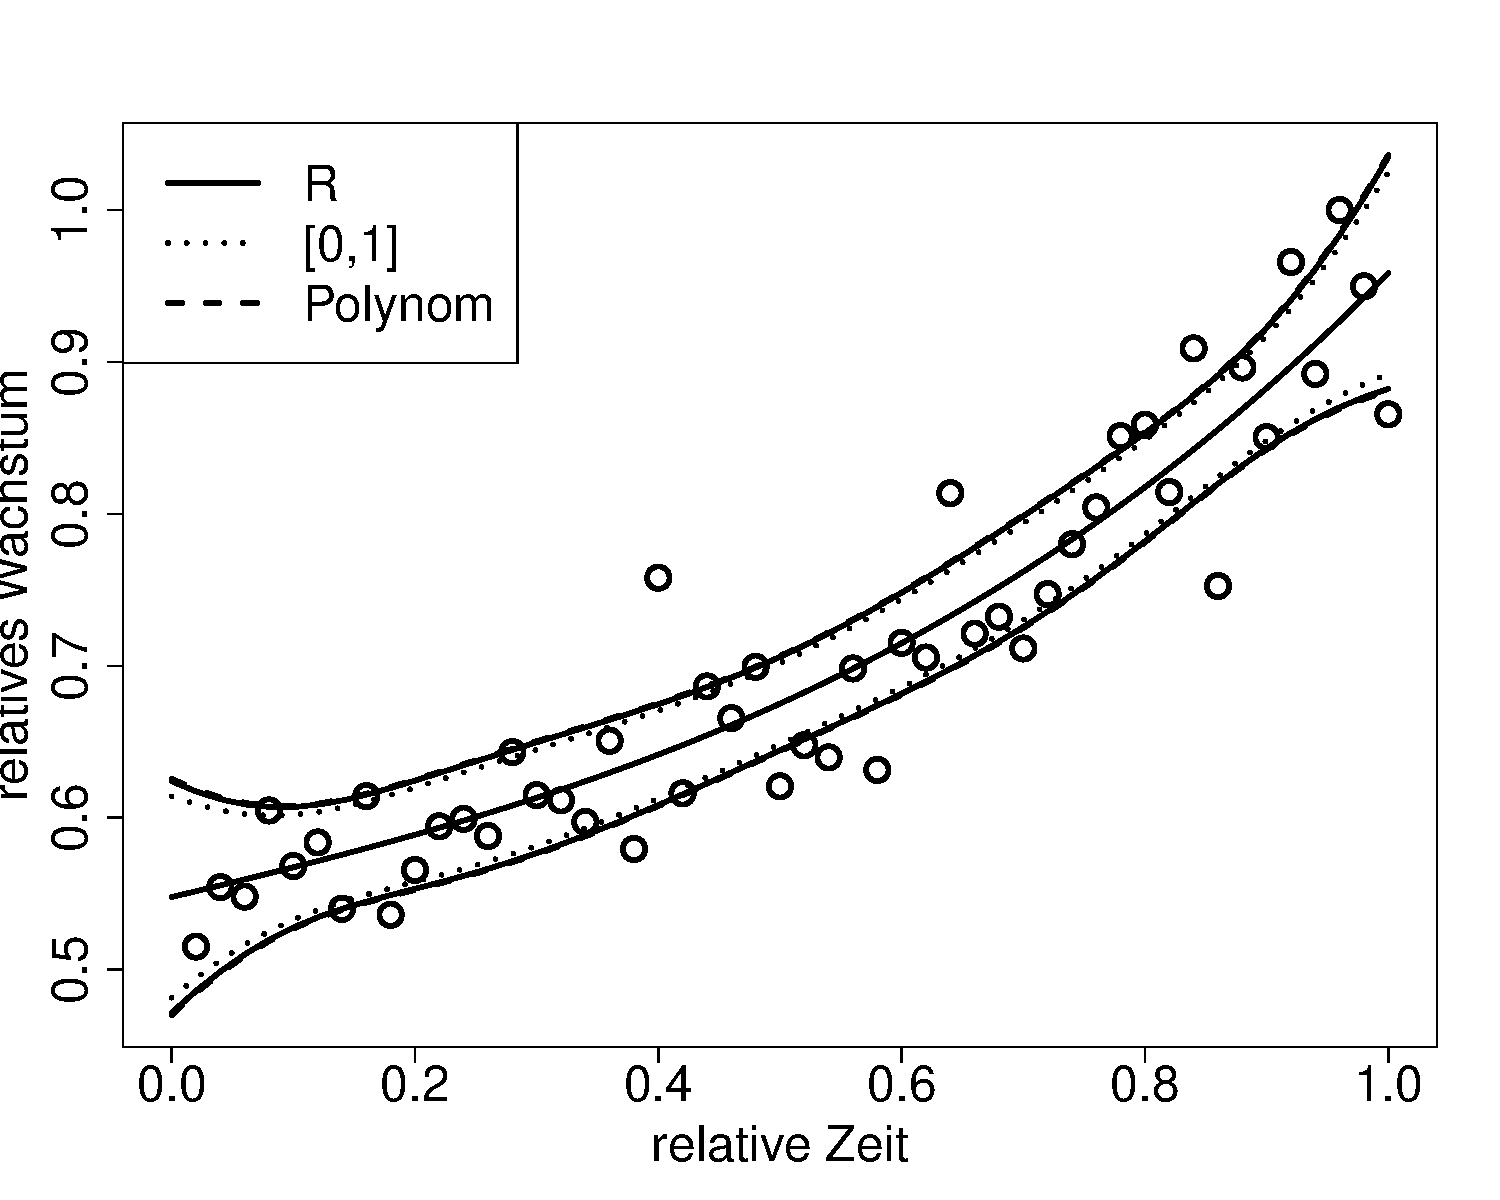
\includegraphics[width=0.5\textwidth]{Bsp-KB-poly}
  \caption{Weiterführung des Beispiels durch Konfidenzband auf [0,1] für Polynome}
  \label{KB-poly-BSP}
\end{figure}

Die kritischen Werte für das Konfidenzband auf ganz $\mathbb{R}$ und für das Konfidenzband auf [0,1] habe ich in den vorherigen Abschnitten bereits berechnet. Es ergaben sich die Werte \cR und \cA . Berechne ich den kritischen Wert für das Konfidenzband auf [0,1], welches die Polynomgestalt berücksichtigt, erhalte ich den Wert \cAP . Dieser Wert ist noch kleiner als der Wert von \cA , was auch zu erwarten war.

Als seed benutze ich, wie gesagt, weiterhin \seedsimulation .

\end{Beispiel}

\begin{Simulation}
Ich beende die Simulationstabelle aus den letzten beiden Abschnitt durch Überdeckungswahrscheinlichkeiten für die Konfidenzbänder auf einem Intervall $A$, in diesem Fall ist wieder $A = \{ (x_1, \ldots, x_p)' : 0 \leq x_i \leq 1, i=1, \ldots, p \}$ aufgrund der Struktur des Modells. Außerdem gehe ich davon aus, dass die Designmatrix Polynomgestalt hat.

\begin{center}
\begin{tabular}{|c|c|c|}
\hline 
$\times$ & R & AR \\ 
\hline 
R		& \UeberRR			& \UeberARR \\ 
\hline 
Minmax	& \UeberRMinmax	 	& \UeberARMinmax \\ 
\hline 
Poly 	& \UeberRMinmaxPoly & \UeberARMinmaxPoly \\ 
\hline 
\end{tabular} 
\end{center}

\end{Simulation}





\newpage
\section{Vergleich von zwei Regressionsmodellen}
\label{Vergleich von zwei Regressionsmodellen}
Da das Ziel dieser Arbeit der Vergleich von Regressionsmodellen ist, wird in diesem Kapitel gezeigt, wie man Regressionsmodelle vergleicht. 

Seien also zwei Regressionsmodelle $ Y_{i} = X_{i} \beta_{i} + e_{i} $ \label{Grundmodell_Hypothesentest} mit $i = 1,2$ gegeben. 

Dabei ist $Y_{i} = (Y_{i,1}, \ldots, Y_{i,n_i})$ ein für $i=1,2$ ein Vektor aus zufälligen Beobachtungen der die abhängigen Daten darstellt.

Weiterhin sei $X_i$ für $i=1,2$ eine $n_i \times (p+1)$ Designmatrix mit vollem Zeilenrang und festem Design. Dabei ist die $j$-te Zeile von $X_1$ mit der $j$-ten Zeile von $X_2$ für $j=1,\ldots \min(n_1,n_2)$ identisch. Diese Bedingung bedeutet, dass beide Designmatrizen das selbe, feste Design haben.

Außerdem sind $\beta_i$ zwei $(p+1) \times 1$ Koeffizientenvektoren, die den funktionalen Zusammenhang zwischen $Y_i$ und $X_i$ darstellen.

In diesem Kapitel ist $e_i \mathscr{N}_{n_i}(0,\sigma^2 I_{n_i})$. Diese Annahme ist wichtig, da sich die Modelle somit nur in $\beta_i$ unterscheiden.

Die zugrunde liegenden Modelle sind also gleich, wenn $\beta_{1}=\beta_{2}$ 

Da die Werte von $\beta_{i}$ unbekannt ist und nur geschätzt werden kann, muss man testen, ob 

\begin{equation}
H_{0} : \beta_{1} = \beta_{2}  \textbf{ vs. }  H_{1} : \beta_{1} \neq \beta_{2} \label{Hypothese}
\end{equation}

Dabei bezeichnet $H_{0}$ die \gls{Nullhypothese} und $H_{1}$ die Alternativhypothese.

Dazu ist es entweder möglich einen Test zu konstruieren oder Konfidenzbänder zu benutzen. Im nächsten Abschnitt wird einen Test konstruieren und im übernächsten Abschnitt Konfidenzbänder benutzt.

Es ist mit der in diesem Kapitel eingeführten Methode auch möglich zwei Modelle mit verschiedenen abhängigen Daten zu vergleichen. 

Ein Beispiel für solch ein vorgehen ist der Vergleich des Blutdrucks von Männern und Frauen. Konkret kann man mit dieser Methode die Frage beantworten, ob sowohl für Männer, als auch für Frauen, der Zusammenhang zwischen zum Beispiel Alter und Blutdruck gleich ist.

\begin{Beispiel}
Es wird das Beispiel aus Kapitel 1 fortgeführt, indem ich eine zweite Designmatrix $X_2$ einführe. Die Designmatrix $X_2$ stellt ein polynomiales Modell vom Grad 3 dar. 

Das heißt, im Beispiel zu diesem Kapitel wird es darum gehen, ob es für die Daten, die ich bereits im ersten Kapitel vorgestellt habe, einen Unterschied macht, ein polynomiales Modell vom Grad Drei oder vom Grad Eins zugrunde zu legen. 

In der folgenden Graphik \ref{Vergleich-Bsp} sind die beiden Modelle mit den Daten eingezeichnet.

\begin{figure}[H] 
  \centering
     \includegraphics[width=0.5\textwidth]{Bsp-beide-in-einem-plot}
  \caption{Regression von Grad Eins und Grad Drei im Vergleich}
  \label{Vergleich-Bsp}
\end{figure}

%Im Folgenden gebe ich die beiden Modelle in Matrixschreibweise an:
%
%\[
%Y = \Ydat = \Xonedat \times \betaonedat + \edat = X_{1} \beta_{1} + e_{1}
%\]
%\[
%Y = \Ydat = \Xtwodat \times \betatwodat + \edat = X_{2} \beta_{2} + e_{2}
%\]
\end{Beispiel}




\subsection{F-Test}
\label{Vergleich F-Test}
Dieser Abschnitt beruht auf \cite[114-115]{Liu64} und \cite{Draper98}

Ich betrachte erst einmal den Test

\begin{equation}
H_{0} : A\beta = b  \textbf{ vs. }  H_{a} : A\beta \neq b \label{Einschränkung_Hypothese}
\end{equation}

Also ob der Parameter in einem gegebenen Regressionsmodell eine lineare Einschränkung erfüllt.

Dazu brauchen ich zuerst den OLS-Schätzer $\hat{\beta}_A$ unter der Bedingung, dass $A \beta = b$. Das heißt $\hat{\beta}_A$ minimiert

\begin{align*}
L(\beta) = (Y-X\beta)'(Y-X\beta) = \Vert Y - X \beta \Vert^2
\end{align*}

über alle $\beta \in \mathbb{R}^{p+1}$, die die Bedingung $A\beta = b$ erfüllen. Man kann $\hat{\beta}_A$ mittels Lagrange-Multiplikatoren finden. 

Betrachte dazu folgenden Satz.

\begin{Satz}
Unter den oben genannten Bedingungen ist der OLS-Schätzer $\hat{\beta}_A$ gegeben durch 
\[
\hat{\beta}_A=(X'X)^{-1}(X'Y+A'c)= \hat{\beta}+(X'X)^{-1}A'c
\]
 mit $c=(A(X'X)^{-1}A')^{-1}(b-A\hat{\beta})$
\end{Satz}

\begin{proof}
\cite[13]{Liu64}
\end{proof}

Bedeutung hat im weiteren der folgende Satz

\begin{Satz}
Unter den oben genannten Bedingungen gilt
\begin{enumerate}
\item $\Vert X \hat{\beta} - X\hat{\beta}_A \Vert^2  \sim \sigma^2 \chi_r^2(\delta)$ mit nicht zentralem Parameter 

$\delta = \Vert X \beta - X E(\hat{\beta}_A \Vert^2 / \sigma^2 = (\beta - E(\hat{\beta}_A))' X'X (\beta - E(\hat{\beta}_A)) / \sigma^2$
\item $\Vert Y - X \hat{\beta}_A \Vert^2  \sim \sigma^2 \chi_{n-(p+1)+r}^2(\delta)$ mit $\delta$ wie in 1.
\item $\Vert X \hat{\beta} - X\hat{\beta}_A \Vert^2$ und $\Vert Y - X \hat{\beta}_A \Vert^2$ sind unabhängig
\item $ \frac{\Vert X \hat{\beta}_A - X\hat{\beta} \Vert^2 / r}{\Vert Y - X \hat{\beta} \Vert^2 / (n-p-1)} \sim f_{p+1,n-p-1}$
\end{enumerate}
\end{Satz}

\begin{proof}
\cite[11]{Liu64}
\end{proof}

Damit kann ich einen Test zum Niveau $1-\alpha$ konstruieren:

\begin{equation}
\textnormal{Lehne }  H_0 \textnormal{ genau dann ab, wenn } \frac{\Vert X \hat{\beta}_A - X\hat{\beta} \Vert^2 / r}{\Vert Y - X \hat{\beta} \Vert^2 / (n-p-1)} > f_{p+1,n-p-1}^{\alpha} \label{Einschränkung_Test}
\end{equation}

Ich werde gleich noch folgenden Satz aus \cite[13]{Liu64} benötigen:

\begin{Satz}
Es gilt 
\[
\Vert X \hat{\beta} - X \hat{\beta}_A \Vert^2 = (A\hat{\beta}-b)'(A(X'X)^{-1}A')^{-1}(A\hat{\beta}-b)
\]
\end{Satz}

\begin{proof}
\cite[13]{Liu64}
\end{proof}


Jetzt werde ich dieses Resultat auf den Vergleich von Regressionsmodellen anwenden. Dabei orientiere ich mich an \cite[114]{Liu64}. Dazu betrachte ich wieder den Test \eqref{Hypothese} :

\begin{equation*}
H_{0} : \beta_{1} = \beta_{2}  \textbf{ vs. }  H_{1} : \beta_{1} \neq \beta_{2}
\end{equation*}

Um einen solchen Test durchzuführen benötigen ich eine Dummyvariable $z$:

\[
z=\begin{cases}
1 & \text{falls Y aus dem Modell 1 ist}\\
0 & \text{falls Y aus dem Modell 2 ist} 
\end{cases}
\]

Mit $z$ kann ich die beiden Modelle zu einem vereinen, indem ich

\begin{equation}
Y = x' c_1 + z x' c_2 + e \label{Grundmodell_umformuliert}
\end{equation}
%= (x',z x') ???(c_1, c_2)??? + e

mit $x=(1,x_1,\ldots,x_p)'$, $c_1=\beta_2$ und $c_2=\beta_1-\beta_2$ setze. Dass dieses Modell mit den beiden Modellen aus \eqref{Grundmodell_Hypothesentest} übereinstimmt, sieht man daran, dass

\begin{equation*}
Y = x'(c_1+c_2)+e = x'\beta_1+e
\end{equation*}

wenn $Y$ aus Modell 1 und 

\begin{equation*}
Y = x'c_1+e = x'\beta_2+e
\end{equation*}

wenn $Y$ aus Modell 2 stammt. Damit kann man den Hypothesentest \eqref{Hypothese} umformulieren zu

\begin{equation*}
H_{0} : c_2 = \beta_1-\beta_2 = 0  \textbf{ vs. }  H_{1} : c_2 \neq 0 
\end{equation*}

Unter $H_{0}$ reduziert sich also das Gesamtmodell \eqref{Grundmodell_umformuliert} zu 

\begin{equation*}
Y = x' c_1 + e
\end{equation*}

Jetzt kann ich \eqref{Einschränkung_Test} benutzen und erhalten als Teststatistik : 

\begin{equation}
\textnormal{Verwerfe } H_0 \textnormal{ genau dann, wenn } 
\frac{(\hat{\beta_1}-\hat{\beta_2})'D (\hat{\beta_1}-\hat{\beta_2})/(p+1)}{\widehat{\sigma^2}} > f^{\alpha}_{p+1,n-p-1}\label{Teststat_final}
\end{equation}

Dabei ist $\hat{\sigma}^2$ die mittlere Varianz des Modells \eqref{Grundmodell_umformuliert}, $\hat{\beta_i} = (X_i'X_i)^{-1}X_iY$ und \gls{D}=$(X_1'X_1)^{-1}+(X_2'X_2)^{-1}$. 

Um zu sehen, dass \eqref{Teststat_final} tatsächlich aus \eqref{Einschränkung_Test} hergeleitet werden kann, betrachten ich die folgende Rechnung nach \cite[115]{Liu64}. Ich betrachte allerdings nur die Berechnung für den Nenner.

%Für den Zähler betrachte:
%
%\begin{eqnarray*}
%X'X = \begin{bmatrix} X'_1 X_1 + X'_2 X_2 & X_1 X_1 \\ X'_1 X_1 & X'_1 X_1  \end{bmatrix} \\
%(X'X)^{-1} = \begin{bmatrix} (X'_2 X_2)^{-1} & -(X_2 X_2)^{-1} \\ -(X'_2 X_2)^{-1} & (X'_1 X_1)^{-1} + (X'_2 X_2)^{-1} \end{bmatrix} \\
%\hat{c} = \\
%\Vert Y - X \hat{c} \Vert^2 =
%\end{eqnarray*}
%
%Beachte, dass in diesem Fall die Matrix $A$ aus dem Test \eqref{Einschränkung_Hypothese} durch die $(p+1) \times 2(p+1)$ Matrix $(0,I_{p+1})$ und der Vektor $b$ durch den Nullvektor gegeben ist. Also ist der Zähler in \eqref{Einschränkung_Test} gegeben durch
%
%\[
%(A\hat{c}-b)'(A(X'X)^{-1}A')^{-1}(A\hat{c}-b)/r = (\hat{\beta}_1 - \hat{\beta}_2)' D (\hat{\beta}_1-\hat{\beta}_2)/(p+1)
%\]

Für den Nenner betrachte

\begin{align*}
\widehat{\sigma^2}  &= \frac{\Vert Y-X \hat{c} \Vert}{n_1 + n_2 - 2(p+1)} \\
				&= \frac{\Vert Y_1 - X_1 \hat{\beta_1} \Vert^2 + \Vert Y_2 - X_2 \hat{\beta_2} \Vert^2}{n_1+n_2-2(p+1)} \\
				&= \frac{n_1-p-1}{n_1+n_2-2(p+1)} \frac{\Vert Y_1 - X_1 \hat{\beta_1} \Vert^2}{n_1-p-1}+ \frac{n_2-p-1}{n_1+n_2-2(p+1)} \frac{\Vert Y_2 - X_2 \hat{\beta_2} \Vert^2}{n_2-p-1} \\
				&= \frac{n_1-p-1}{n_1+n_2-2(p+1)} \hat{\sigma_{1}^2}+ \frac{n_2-p-1}{n_1+n_2-2(p+1)} \hat{\sigma_{2}^2}
\end{align*}

Ich führe nun das Beispiel aus der Einleitung zu diesem Kapitel fort

\begin{Beispiel}
Berechnet man die Teststatistik \eqref{Teststat_final} erhält man als Teststatistik den Wert ... und als kritischen Wert ... . Also ... man die Hypothese. Die Modelle sind also ... .
\end{Beispiel}

Allerdings macht solch ein Test keinerlei Aussage über die Größe des Unterschiedes zwischen den Modellen. Deshalb nutze ich im nächsten Abschnitt die Ergebnisse aus Kapitel \ref{Regression und Konfidenzbaender}.


\subsection{Vergleich von Regressionsmodellen mit Konfidenzbändern}
\label{Konfidenzbaender vergleich}
Dieser Abschnitt basiert auf \cite[119-121]{Liu64}
Die grundlegende Idee ist, die Modelle voneinander abzuziehen und dann zu sehen, ob die Nullfunktion in einem Konfidezband um die Differenz der beiden Modelle liegt.

Ich formalisiere dies nach \cite[122]{Liu64}: 

Ein zweiseitiges, hyperbolisches, gleichmäßiges Konfidenzband für $x'\beta_2 - x'\beta_1$ über der Region $A$ hat die Form

\begin{equation} \label{Vergleich-KB}
x'\beta_2-x'\beta_1 \in x' \hat{\beta}_1 - x' \hat{\beta}_2 \pm c ~ \hat{\sigma} \sqrt{x' D x} ~ \text{ für alle } x \in A
\end{equation}

wobei $c$ eine kritische Konstante ist, sodass das Konfidenzniveau des Konfidenzbandes $1-\alpha$ beträgt. Dabei ist $D = (X_1'X_1)^{-1} + (X_2'X_2)^{-1}$

Sei $P$ die eindeutig bestimmte Wurzel aus $D = (X_1'X_1)^{-1} + (X_2'X_2)^{-1}$ wie im ersten Kapitel und definiere $T=P^{-1}(\hat{\beta}_2 - \beta_2 - \hat{\beta}_1 + \beta_1)/\hat{\sigma}$ welches wieder die $\tau_{p+1,v}$ Verteilung besitzt. Es folgt wie in Kapitel 1.4, dass das Simultane Konfidenzband \eqref{Vergleich-KB} gegeben ist durch $\mathbb{P}(S<c)$ mit

\begin{eqnarray*}
S &=& \sup_{x \in A} \frac{x' (\hat{\beta}_2-\beta_2-\hat{\beta}_1+\beta_1)}{\hat{\sigma}\sqrt{x' D x}}\\
&=& \sup_{x \in A} \frac{(Px)' (P^{-1} (\hat{\beta}_2-\beta_2-\hat{\beta}_1+\beta_1)/\hat{\sigma}}{\sqrt{(Px)'(Px)}} \\
&=& \sup_{x \in A} \frac{\vert (Px)' T \vert}{\Vert Px \Vert}
\end{eqnarray*}

Also kann die kritische Konstante $c$ genauso wie in Kapitel 1.4 beziehungsweise wie in Kapitel 1.5 gefunden werden.

Der folgende Satz zeigt, dass es keinen Unterschied macht, ob ich einen F-Test durchführe oder ein Konfidenzband auf ganz $\mathbb{R}$ benutze.

\begin{Satz}
F-Test und Konfidenzbandmethode auf ganz $\mathbb{R}$ liefern immer das selbe Ergebnis, das heißt sie widerlegen beziehungsweise bejahen einen Test genau dann wenn der andere ihn auch widerlegt beziehungsweise bejaht.
\end{Satz}

\begin{proof}
\cite[67]{Liu64}
\end{proof}

Das heißt, dass es von einem Interferenzstandpunkt her immer besser ist, ein Konfidenzband zum Vergleich von zwei Modellen zu verwenden.

Weiterhin hatte ich bereits im ersten Kapitel gezeigt, dass Konfidenzbänder auf einem Intervall und erst recht Konfidenzbänder für Polynome auf einem Intervall eine bessere Inferenz zulassen, als Konfidenzbänder auf ganz $\mathbb{R}$. Also ist es immer von Vorteil Konfidenzbänder auf Intervallen zu verwenden.

%Was passiert, wenn eines der Modelle weniger Dimensionen (im Sinne der Designmatrix) als das andere hat ?

\begin{Beispiel}
Ich führe jetzt das Beispiel aus den vorherigen Abschnitten fort, indem ich die Differenz der Regressionsmodelle plotte und Konfidenzbänder auf [min(X),max(X)] für Polynome einfüge

\begin{figure}[H] 
  \centering
     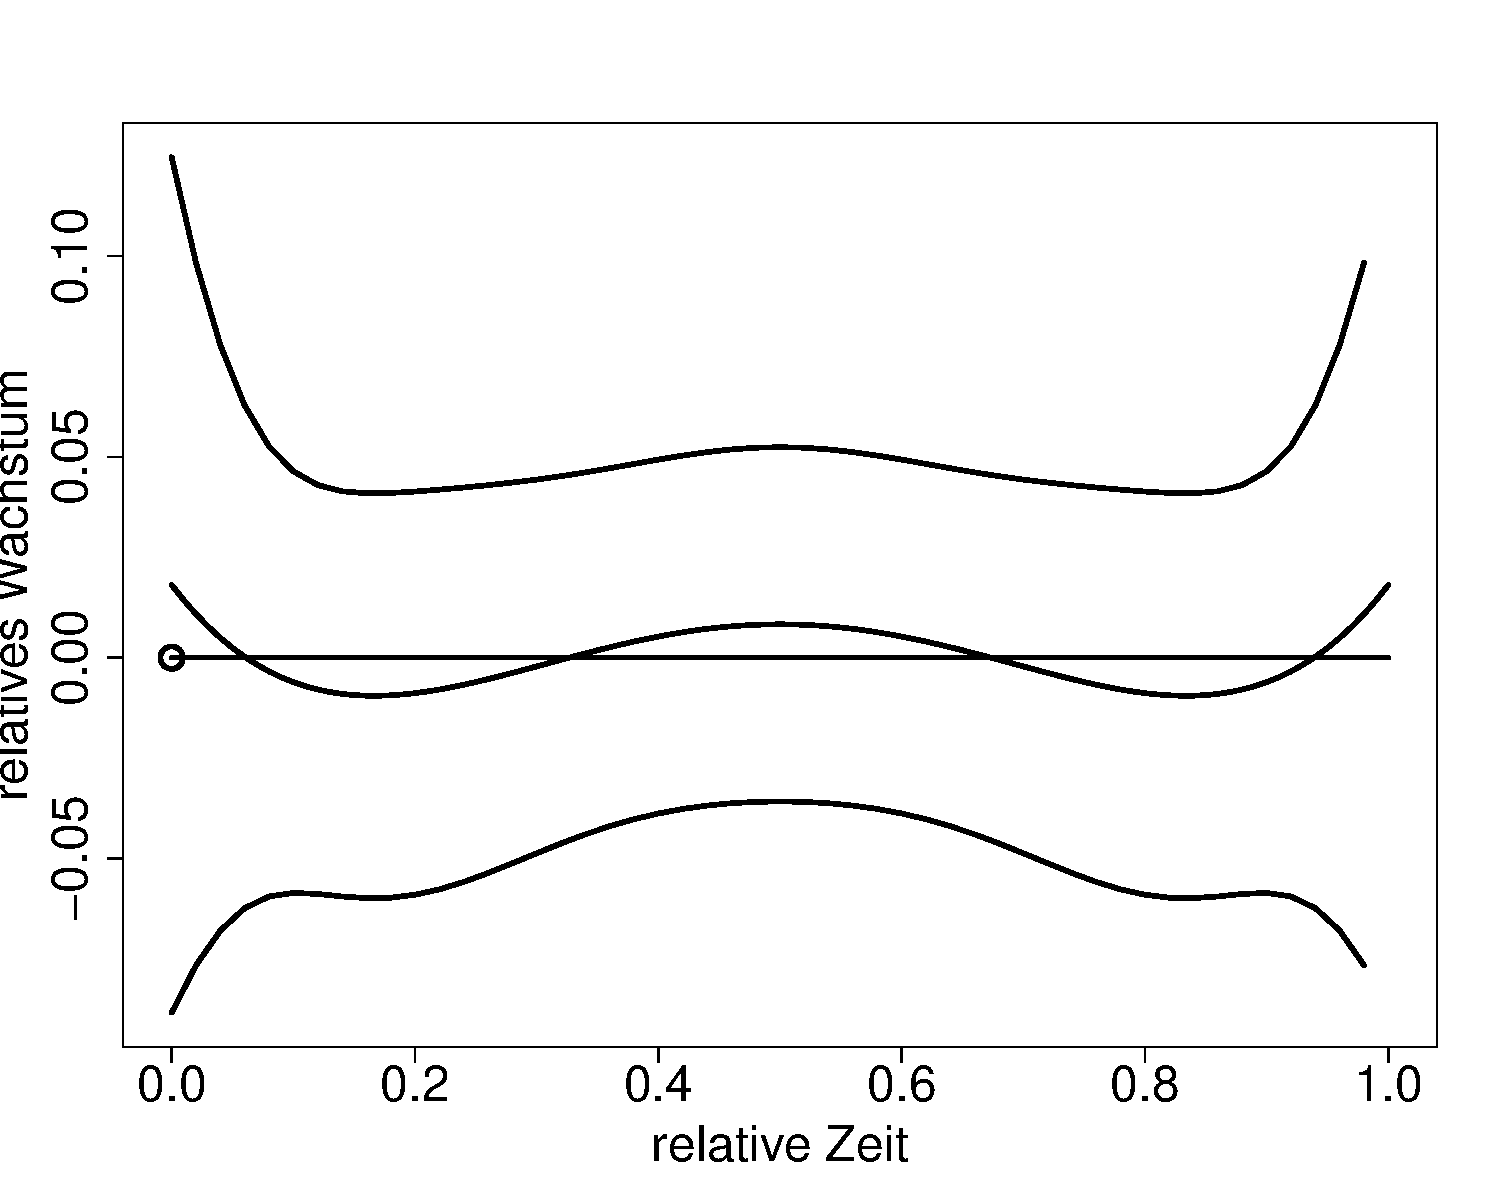
\includegraphics[width=0.5\textwidth]{Bsp-KB-poly-hetero}
  \caption{Differenz des Beispiels mit Konfidenzbandauf [min(X),max(X)] für Polynome in AR(1)}
  \label{KB-poly-hetero-BSP}
\end{figure}

Man sieht, dass ...

\end{Beispiel}


%\subsection{Konfidenzbänder auf einem Intervall}
%\label{Vergleich Konfidenzbaender auf einem Intervall}
%Dieser Abschnitt orientiert sich an \cite[121-123]{Liu64} und \cite{Jamshidian07} und \cite{Liu07}.
%
%
%\subsection{Konfidenzbänder auf einem Intervall, wenn das Regressionsmodell Polynomgestalt hat}
%\label{Vergleich Konfidenzbaender auf einem Intervall, wenn das Regressionsmodell Polynomgestalt hat}
%Dieser Abschnitt orientiert sich an \cite[197-200]{Liu64}.


\newpage
\section{Teil eines Regressionsmodells überprüfen}
\label{Teil eines Regressionsmodells überprüfen}
In diesem Abschnitt wird der Spezialfall zu prüfen, ob ein Teil des Regressionsmodells signifikant von Null verschieden ist oder nicht.  Das heißt, wir gehen von dem Modell

\begin{equation} \label{RegprüfModell}
Y=X \beta + e
\end{equation}

und wollen prüfen, ob einige der Koeffizienten $\beta_i$ gleich Null sind oder nicht. Ist $\beta_i$ gleich Null haben die zugehörigen unabhängigen Variablen $x_i$s keinen Einfluss auf die abhängige Variable $Y$. 

Zu diesem Zweck unterteilen wir den Vektor $\beta=(\beta_1,\beta_2)$ mit $\beta_1=(\beta_0, \ldots, \beta_{p-k})$ und $\beta_2=(\beta_{p-1+1}, \ldots, \beta_{p})$ für $1 \leq k \leq p$ eine gegebene natürliche Zahl. 

Auf die gleiche Art und Weise kann man die Spalten $x$ von $X$ in $x_1=(1,x_1, \ldots, x_{p-k})$ und $x_2=(1,x_{p-k+1}, \ldots, x_{p})$ unterteilen.

Ist $\beta_2=0$ so haben die unabhängigen Variablen $x_{p-k+1}, \ldots, x_p$ keinen Einfluss auf $Y$ und man kann das Modell \ref{RegprüfModell} auf 

\begin{equation}
Y=X_1 \beta_1 + e
\end{equation}

vereinfachen. Dabei ist $X_1$ die Matrix die von den ersten $p-k+1$ Spalten von $X$ geformt wird.

\subsection{F-Fest}
\label{F-Test-Teil}
In diesem Abschnitt wird der F-Test als Methode, um zu prüfen, ob $\beta_2=0$ ist, vorgestellt. Dieser Abschnitt orientiert sich an \cite[100-102]{Liu64}.

Ein Ansatz zu prüfen ob $\beta_2=0$ ist, ist der Test 

\begin{equation} \label{Test_prüfen}
H_{0} : \beta_{2} = 0  \textbf{ vs. }  H_{1} : \beta_{2} \neq 0
\end{equation}

der auch in \cite{Draper98} vorgeschlagen wird. Analog zu Abschnitt \ref{Vergleich F-Test} erhält man die Teststatistik

\begin{equation*}
\frac{(\tilde{I}\hat{\beta})'(\tilde{I}(X'X)^{-1}\tilde{I}')^{-1}(\tilde{I}\hat{\beta})/k}{\text{mean square residual von Modell \ref{RegprüfModell}}} > f^{\alpha}_{k,v}
\end{equation*}

mit $v=n-p-1$, $\tilde{I}$ der $k \times (p+1)$ Matrix die durch $\tilde{I}=(0,I_k)$ gegeben ist und $f^{\alpha}_{k,v}$ dem $\alpha$ Quantil der $f$ Verteilung mit $k$ und $v$ Freiheitsgraden.

Dabei ist der MS residual von Modell \eqref{RegprüfModell} gegeben durch

\begin{equation*}
\text{MS} = \Vert Y - X\hat{\beta} \Vert^2 / (n-p-1) = \hat{\sigma}
\end{equation*}

Lehnt man bei diesem Test die Nullhypothese ab, heißt dies, dass es nicht genug statistisch gesicherte Hinweise gibt, um anzunehmen, dass $\beta_{2} = 0$ ist. Dies heißt allerdings nicht, dass wir davon ausgehen können, dass $\beta_2 \neq 0$ ist. 

Benutzt man stattdessen ein Konfidenzband hat man ein Maß für den Unterschied der Modelle und kann eher entscheiden, ob $\beta_2 \neq 0$. Der nächste Satz gibt genau solch ein Theorem an

\begin{Satz}
Es gilt
\begin{equation} \label{KB_R_prüfen}
\mathbb{P}(x_2'\beta_2 \in x_2'\hat{\beta_2} \pm \sqrt{k f^{\alpha}_{k,n-p-1}} \hat{\sigma} \sqrt{x_2' V x_2}) = 1 - \alpha
\end{equation}
\end{Satz}

Dabei ist $V=\tilde{I}(X'X)^{-1}\tilde{I}'$, $\hat{\beta_2} = \tilde{I} \hat{\beta}$ mit $\tilde{I}$ wie oben. Dieser Satz kann ähnlich wie Satz \eqref{KB_Eigenschaft} bewiesen werden. Außerdem gilt folgender Satz

\begin{Satz}
Test \eqref{Test_prüfen} und das Konfidenzband \eqref{KB_R_prüfen} verwerfen und akzeptieren $H_0$ zur selben Zeit.
\end{Satz}

Das Konfidenzband \eqref{KB_R_prüfen} gibt einem also immer mehr Information. Allerdings ist das Konfidenzband auf ganz $R^k$ definiert. Eine noch besser Aussage über $H_0$ kann man also treffen, wenn man stattdessen ein Konfidenzband auf $A$ betrachtet. 

\subsection{Teil eines Regressionsmodells auf einem Intervall überprüfen}
\label{Teil eines Regressionsmodells auf einem Intervall überpruefen}
Dieser Abschnitt orientiert sich an \cite[102-105]{Liu64}.

Wir beschränken uns auf die rechteckige Region

\begin{equation*}
A_2 = \{ x_2 \in \mathbb{R}^k =(x_{2,p-k+1}, \ldots x_{2,p}) : x_{2,1} \in [a_i,b_i], i=p-k+1, \ldots, p \}
\end{equation*}

dabei sind $- \infty \leq a_i \leq b_i \leq \infty, i = p-k+1, \ldots, p$ gegebene Konstanten. Ein hyperbolisches Konfidenzband auf $A_2$ ist gegeben durch

\begin{equation}\label{KB_pruefen}
x_2'\beta_2 \in x_2'\hat{\beta_2} \pm c \hat{\sigma}\sqrt{x_2'Vx_2} \text{ für alle } x_2 \in A_2
\end{equation}

dabei muss man die kritische Konstante $c$ so bestimmen, dass das gleichmäßige Konfidenzniveau $1 - \alpha$ ist.

Sei $W$ die Wurzel aus $V$, also sei $V=W^2$. Bezeichne $N_2=W^{-1}(\hat{\beta_2}-\beta_2)/\sigma \sim \mathscr{N}_k(0,I)$ und $T_2 = N_2/(\hat{\sigma}/\sigma \sim \tau_{k,v}$. Dann ist das Konfidenzlevel von \eqref{KB_pruefen} gegeben durch $\mathbb{P}(S<c)$ wobei

\begin{eqnarray*}
S &=& \sup_{x_2 \in A_2} \frac{\vert x_2' (\hat{\beta_2} - \beta_2) \vert }{\hat{\sigma} \sqrt{x_2' V  x_2}} \\
&=& \sup_{x_2 \in A_2} \frac{\vert (Wx_2)'W^{-1} (\hat{\beta_2}-\beta_2)/\hat{\sigma} \vert}{\sqrt{(Wx_2)'(Wx_2)}} \\
&=& \sup_{v \in C(W,A_2)} \frac{\vert v'T_2 \vert }{\Vert v \Vert}
\end{eqnarray*}

wobei $C(W,A_2)=\{ \lambda W x_2 = \lambda(x_{p-k+1} w_1 + \ldots + x_p w_k) : \lambda > 0 \text{ and } x_2 \in A_2 \}$ mit $W=(w_1, \ldots, w_k)$. 

Die Verteilung von $S$ hängt nicht von $\beta$ und $\sigma$ ab. Allerdings hängt sie in komplizierter Weise von der Region $A_2$ und $W$ durch $C(W,A_2$ ab.

Für die beiden Spezialfälle $k=1$ und $0 \in C(W,A_2)$ ergeben sich Vereinfachungen. Im allgemeinen Fall kann man $c$ ähnlich wie in Abschnitt \ref{Konfidenzbaender auf einem Intervall fuer ein multiples lineares Regressionsmodell} finden. Dazu berechnet man $R$ mal $S_i$ auf die folgende Art:

\begin{enumerate}
\item Simuliere $N_2 \sim \mathscr{N}_k(0,I)$ und $\hat{\sigma}/\sigma \sim \sqrt{\chi^2_v/v}$
\item Bestimme $\Vert \pi^{*}(T_2,W,A_2) \Vert$ und $\Vert \pi^{*}(-T_2,W,A_2) \Vert$
\item Dann ist $S= \max(\Vert \pi^{*}(T_2,W,A_2) \Vert, \Vert \pi^{*}(-T_2,W,A_2) \Vert )$
\end{enumerate}

Dann ist die kritische Konstante $c$ das $1-\alpha$ Quantil von $S_1, \ldots, S_R$.

Die Berechnung von $\Vert \pi^{*}(T_2,W,A_2) \Vert$ findet man in \cite[Appendix B]{Liu64}.

Ich habe diese Methode nicht weiter verfolgt, da das Ziel dieser Arbeit ist Konfidenzbänder zu vergleichen. Außerdem werden im letzten Kapitel Datenbeschreibung und Resultate vor allem Polynommodelle betrachtet. Wie man in diesem Fall Konfidenzbänder konstruiert ist Thema des nächsten Abschnitts.

\begin{Simulation}
Ich habe für das Konfidenzband auf ganz $\mathbb{R}^n$ wieder eine Simulation für die Überdeckungswahrscheinlichkeit für Daten aus einer gewöhnlichen multilinearen Regression und einer Regression mit AR(1)-Kovarianzmatrix durchgeführt:

\begin{center}
\begin{tabular}{|c|c|c|}
\hline 
$\times$ & R & AR \\ 
\hline 
R		& \UeberRR			& \UeberARR \\ 
\hline 
Minmax	& \UeberRMinmax	 	& \UeberARMinmax \\ 
\hline 
Poly 	& \UeberRMinmaxPoly & \UeberARMinmaxPoly \\ 
\hline 
R prüfen	& \UeberRRpruefen & \UeberARRpruefen \\ 
\hline 
\end{tabular} 
\end{center}

\end{Simulation}



\subsection{Teil eines Regressionsmodells überprüfen, wenn das Modell Polynomgestalt hat}
\label{Teil eines Regressionsmodells überpruefen, wenn das Modell Polynomgestalt hat}
Dieser Abschnitt orientiert sich an \cite[190-192]{Liu64} und \cite{Draper98}.

Für den Fall, dass man Modelle mit Polynomgestalt betrachtet erhält man als $f$-Test

\begin{equation}\label{KB hypo prüfen}
\text{reject } H_0 \leftrightarrow \frac{\hat{\beta_2}' V^{-1} \hat{\beta_2}/k}{\widehat{\sigma^2} > f^{\alpha}_{k,v}}
\end{equation}

mit $\hat{\beta_2}$ ist der Schätzer für $\beta_2=(b_{p-k+1}, \ldots b_{p})'$ welcher die letzten $k$ Komponenten ist und Verteilung $\mathscr{N}(\beta_2,\sigma^2,V)$. Außerdem ist $V$ die $k \times k$ Matrix, die von den letzten $k$ Zeilen und den letzten $k$ Spalten von $(X'X)^{-1}$, erzeugt wird. Da $V$ nicht singulär ist, sei $W$ die eindeutig bestimmte Wurzel von $V$, dass heißt $V=W^2$. 

Analog zum letzten Abschnitt kann wieder gezeigt werden, dass dieser Test dem Konfidenzband 

\begin{equation}\label{KB poly prüfen}
x_2' \beta_2 \in x_2' \hat{\beta_2} \pm \sqrt{k f^{\alpha}_{k,v}} \hat{\sigma} \sqrt{x_2' V x_2} \text{ für alle } x_2 \in \mathbb{R}^k
\end{equation}

entspricht. Das heißt liegt die Nullfunktion nicht vollständig in dem Konfidenzband \eqref{KB poly prüfen}, kann man die Nullhypothese aus Test \eqref{KB hypo prüfen} ablehnen.

Analog zu Abschnitt \ref{Konfidenzbaenderauf auf einem Intervall für Regressionsmodell mit Polynomgestalt} kann man wieder ein Konfidenzband auf einem Intervall $A$ konstruieren, dass die polynomstruktur berücksichtigt.

Dazu betrachtet man, dass das Konfidenzniveau von \eqref{KB poly prüfen} für $c$ anstatt $\sqrt{k f^{\alpha}_{k,v}}$ durch $\mathbb{P}(S\leq c)$ gegeben ist. Dabei ist

\begin{eqnarray*}
S &=& \sup_{x \in A} \frac{\vert \tilde{x_2}' (\hat{\beta_2}-\beta_2)}{\hat{\sigma} \sqrt{\tilde{x_2'}V\tilde{x_2}}} \\
&=& \sup_{x \in A} \frac{\vert (1, \ldots, x^{k-1})(\hat{\beta_2}-\beta_2}{\hat{\sigma} \sqrt{(1, \ldots, x^{k-1}) V (1, \ldots x^{k-1})'}}
\end{eqnarray*}

mit $\tilde{x_2}= x^{p-k+1}(1, x, \ldots, x^{k-1})$.

Also ist die kritische Konstante $c$ genau so wie in Abschnitt \ref{Konfidenzbaenderauf auf einem Intervall für Regressionsmodell mit Polynomgestalt} berechenbar, außer dass man $p=k-1$ und $(X'X)^{-1}$ mit $V$ ersetzen muss. Die Simulation ändert sich allerdings nicht.

\begin{Simulation}
Auch für die Methode aus diesem Abschnitt habe ich Simulationen durchgeführt:

\begin{center}
\begin{tabular}{|c|c|c|}
\hline 
$\times$ & R & AR \\ 
\hline 
R		& \UeberRR			& \UeberARR \\ 
\hline 
Minmax	& \UeberRMinmax	 	& \UeberARMinmax \\ 
\hline 
Poly 	& \UeberRMinmaxPoly & \UeberARMinmaxPoly \\ 
\hline 
R prüfen	& \UeberRRpruefen & \UeberARRpruefen \\ 
\hline 
Poly prüfen	& \UeberRMinmaxPolypruefen & \UeberARMinmaxPolypruefen \\ 
\hline 
\end{tabular} 
\end{center}

\end{Simulation}

%\subsection{Ausblick: Vergleich mit der Nullfunktion}
%\label{Ausblick: Vergleich mit der Nullfunktion}
%Dieser Abschnitt orientiert sich an \cite[110-112]{Liu64}.


\newpage
\section{Regression und Konfidenzbänder für abhängige Daten}
\label{Regression und Konfidenzbänder für abhaengige Daten}
Alle bisherigen Ergebnisse beruhen auf dem homoskedastischem, multiplen linearen Modell. Das heißt, mit $Y \in \mathbb{R}^n$, $\beta \in p$ und $X \in n \times p$ wurde von dem funktionalem Zusammenhang

\begin{align} \label{Grundmodell_AR}
Y = X \beta + e
\end{align}

ausgegangen, wobei $e \sim \mathscr{N}_0,I_n \sigma^2)$ war.  Es wurden für dieses Modell Konfidenzbänder mit verschiedenen Designmatritzen $X$ sowohl auf $\mathbb{R}^{n}$ als auch auf einem Intervall $A$ bestimmt.

In diesem Kapitel wird der Fall betrachtet, dass die Fehler untereinander korreliert sind. 

Zuerst betrachten wir, wie man in diesem Fall die Parameter des Modells schätzten kann. Danach konstruieren wir für das Modell Konfidenzbänder. 

Dieses Kapitel orientiert sich an \cite{Hansen15} und  \cite{Pinheiro00}.


\subsection{Regression für AR(1)}
\label{Regression für AR(1)}
In diesem Abschnitt wird das Modell \eqref{Grundmodell_AR} auf den Fall von abhängigen Daten verallgemeinert. Daten sind abhängig, wenn $\text{Cov}(y_i,y_j) \neq 0$ für $i \neq j$.

Insbesondere werden Zeitreihen betrachtet. Eine Zeitreihe ist eine Reihe von Messungen an Zeitpunkten $ t=1, \ldots, T $. Im Folgenden bedeutet der Index $t$, dass es sich um eine Messung handelt und $T$ ist die Anzahl an Messungen. 

Da die Messungen nacheinander getätigt werden, steht zu vermuten, dass $y_t$ und $y_{t+1}$ auf irgendeine Art und Weise nahe beieinander sind. Ist dies der Fall, sind $y_t$ und $y_{t+1}$ nicht unabhängig. Unabhängigkeit war allerdings eine der zentrale Annahmen im ersten Kapitel. Deshalb muss man Schätzer für die Parameter des Modells auf eine andere Art bestimmen.

Es gibt verschiedene Arten von Zeitreihen. Uns werden im folgenden nur Zeitreihen der Form 

\begin{align}
y_t = \phi y_{t-1} + e_t
\end{align}

interessieren. Dabei ist \gls{phi} ein unbekannter Parameter und $\mathbb{E}(e_t)=0$, $\mathbb{E}(e_t^2)=\sigma^2 < \infty$.

Bei solchen Zeitreihen hängt der Wert zur Zeit $t$ offenbar vom Wert der Zeitreihe zur Zeit $t-1$ ab. Somit ist hier $\text{Cov}(y_i,y_j) \neq 0$ für $i \neq j$ und die Ergebnisse aus Kapitel 1 können nicht angewendet werden. 

Eine Zeitreihe dieser Form nennt man einen autoregressiven Prozess erster Art (AR(1)).

Man kann $\text{Cov}(Y_i,Y_j)$ durch den funktionalen Zusammenhang $Y_i = \phi^{j-i} Y_j$ für $i>j$ finden. Für $j<i$ ist $Y_j = \phi^{i-j} Y_i$. 

Beispielsweise erhält man für $i=1$ den Zusammenhang $Y_1 = \phi^j Y_j$ und somit:

\begin{eqnarray*}
\text{Cov}(Y_1,Y_j) &=& \mathbb{E}((\mathbb{E}(Y_1)-Y_i)(\mathbb{E}(Y_j)-Y_j)) \\
&=& \mathbb{E}(\mathbb{E}(Y_1)\mathbb{E}(Y_j) - \mathbb{E}(Y_1)Y_j - \mathbb{E}(Y_j)Y_i +Y_j Y_1) \\
&=& \phi^j \mathbb{E}(\mathbb{E}(Y_j^2) - 2 \mathbb{E}(Y_j)Y_j + Y_j^2) \\
&=& \phi^j \mathbb{E}(\mathbb{E}(Y_j^2)-\mathbb{E}(Y_j)^2) \\
&=& \phi^j \sigma^2
\end{eqnarray*}

Damit hat die Kovarianzmatrix \gls{Xi} von $e$ in diesem Fall die Form:

\[
\Upsilon = 
\left[
   \begin{array}{cccccc}
     1 				& \phi 			& \phi^2	& \cdots	& \phi^{n-2}	& \phi^{n-1} 	\\
     \phi 			& 1		 		& \phi 		& \cdots	& \phi^{n-3}	& \phi^{n-2} 	\\
     \phi^2 		& \phi 			& 1		 	& \ddots	& \vdots		& \vdots 		\\
     \vdots		 	& \vdots	 	& \ddots	& \ddots	& \phi			& \phi^{2} 	\\
     \phi^{n-2} 	& \phi^{n-3}	& \cdots 	& \phi		& 1				& \phi 		\\
     \phi^{n-1} 	& \phi^{n-2} 	& \cdots	& \phi^{2}	& \phi			& 1  
   \end{array}
\right]
\]

Das heißt, das Modell ist gegeben durch 

\begin{align} \label{AR Modell}
Y = X \beta + e
\end{align}

mit $e \sim \mathscr{N}_(0,\Upsilon)$.

Für ein solches Modell ist bisher nicht klar, wie man einen ML-Schätzer bestimmt. Allerdings kann man folgenden Trick anwenden, um die Ergebnisse aus dem ersten Kapitel doch anwenden zu können: Man multipliziert beide Seiten der Gleichung mit $\Upsilon^{-1/2}$. Dann wird aus dem Modell \eqref{AR Modell} wieder das Modell \eqref{Grundmodell_AR}, wenn auch mit anderen Werten. Konkret erhält man

\begin{align} \label{AR rück}
(\Upsilon^{-1/2})Y = Y^{*} = X^{*} \beta + e^{*} = (\Upsilon^{-1/2})X + (\Upsilon^{-1/2})e
\end{align}

mit $e^{*} = (\Upsilon^{-1/2})e \sim \Upsilon^{-1/2} \cdot \mathscr{N}_(0,\Upsilon) = \mathscr{N}_0,\Upsilon^{-1}\Upsilon) = \mathscr{N}_(0,I)$. Die Schwierigkeit besteht also darin, die Konstante $\phi$ zu bestimmen. Ich gehe hier nicht weiter darauf ein, sondern verwende einfach die Funkion \textbf{gls} aus dem \textit{nlme} Paket. Bei der Benutzung von \textit{gls} um $\phi$ zu bestimmen, muss der Wert \textit{correlation=corAR1()} an \textit{gls} übergeben werden.

Konkret berechne ich 

\begin{enumerate}
\item Ich benutze gls um $\phi$ zu bestimmen.
\item Ich bestimme $\Upsilon$ und mittels der R-Funktion \textit{solve} $\Upsilon^{-1}$ 
\item Ich führe eine Eigenwertzerlegung von $\Upsilon^{-1}$ durch um die Matrix zu diagonalisieren und nehme dann von der Hauptdiagonalenmatrix elementenweise die Wurzel, um $\Upsilon^{-1/2}$ zu bestimmen.
\item Ich transformiere $Y$ nach $Y^{*}$ und $X$ nach $X^{*}$ mittels Linksmultiplikation mit $\Upsilon^{-1/2}$
\item Ich benutze eine normale OLS um $D=(X^{'*}X^{*})^{-1}$, $\beta$ und $\sigma^2$ zu berechnen. Dabei müsste $\sigma^2 = 1 $ wegen der Transformation sein.
\end{enumerate}

Führt man diese Schritte durch, das heißt man transformiert die Daten und berechnet dann den OLS Schätzer 

\begin{equation*}
\hat{\beta} = (X^{t} X)^{-1} X^{t} Y
\end{equation*}

für die transformierten Daten 

\begin{equation*}
\Upsilon^{-1/2} Y = \Upsilon^{-1/2} X \beta + \Upsilon^{-1/2} e
\end{equation*}

erhält man :

\begin{eqnarray*}
\hat{\beta} &=& ((\Upsilon^{-1/2} X)^{t} \Upsilon^{-1/2} X)^{-1} (\Upsilon^{-1/2} X)^{t} \Upsilon^{-1/2} Y \\
&=& (X^{t} \Upsilon^{-1/2} \Upsilon^{-1/2})^{-1} X^{t} \Upsilon^{-1/2} \Upsilon^{-1/2} Y \\
&=& (X^{t} \Upsilon^{-1} X)^{-1} X^{t} \Upsilon^{-1} Y
\end{eqnarray*}
 
Was genau der generalised least squares (gls) Schätzer ist.

In einigen Versuchen war dieser Schätzer mit dem Schätzer aus der Funktion \textit{gls} aus dem \textit{nlme} Paket identisch. Deswegen wird in Zukunft immer direkt der Schätzer aus dem gls Paket benutzt.

Dieses Vorgehen hat bei den Simulationen die Überdeckungswahrscheinlichkeit um bis zu ein Prozent erhöht.

Dies ist vor allem praktisch, da es mir bisher nicht möglich war den Parameter $\phi$ der Regression auszulesen. Der Parameter sollte in \textit{corStruct} in \textit{modelStruct} zu finden sein. Dort war er bisher leider nicht zu finden. 

\begin{Beispiel}
Jetzt wird das Beispiel aus dem Abschnitt \ref{Regression} fortgeführt, indem eine Regression mit AR(1) für das Polynommodell mit Grad Eins durch geführt wird. 

Man erhält als Schätzer für den AR(1) Parameter $\hat{\phi}$ = \phiestone , während der wahre Wert \phitrue ist. Dieser Wert ist ... von dem wahren Wert entfernt. Der Schätzer für $\phi$ ist also ... .

Als Schätzung für die Parameter erhält man \betaARone und \sigmaARone , während die wahren Werte \betatrue und \sigmatrue sind . Diese Schätzer sind ... .

%und entsprechend die \nobs $\times$ \nobs Matrix
%
%\[
%\Xidat
%\]
%
%Als nächstes transformiere ich $Y$ nach $Y^{*}$ mittels Linksmultiplikation mit $Xi$
%
%\begin{align*}
%\Upsilon^{-1/2} \times Y &=& \\
% \left[ \begin{array}{ccccccc} 1.00 & 2e^{-2} & -1e^{-4} & 2e^{-6} & -4e^{-8} & 8e^{-10} & -2e^{-11}  \\ 1.00 & 2e^{-2} & -1e^{-4} & 2e^{-6} & -4e^{-8} & 8e^{-10} & -2e^{-11}  \\ 1.00 & 2e^{-2} & -1e^{-4} & 2e^{-6} & -4e^{-8} & 8e^{-10} & -2e^{-11}  \\ 1.00 & 2e^{-2} & -1e^{-4} & 2e^{-6} & -4e^{-8} & 8e^{-10} & -2e^{-11}  \\ 1.00 & 2e^{-2} & -1e^{-4} & 2e^{-6} & -4e^{-8} & 8e^{-10} & -2e^{-11}  \\ 1.00 & 2e^{-2} & -1e^{-4} & 2e^{-6} & -4e^{-8} & 8e^{-10} & -2e^{-11}  \\ 1.00 & 2e^{-2} & -1e^{-4} & 2e^{-6} & -4e^{-8} & 8e^{-10} & -2e^{-11}   \end{array} \right]
%\times 
%\left[ \begin{array}{c} 1 \\ 2 \\ 8 \\ 14 \\ 9 \\ 13 \\ 18 \\ 12 \\ 20 \\ 24 \end{array} \right] \\
%&=& ... = Y^{*}
%\end{align*}
%
%
%und ich transformiere $X$ nach $X^{*}$
%
%\[
%\Upsilon^{-1/2} \times X = ... = ... = X^{*}
%\]
%
%als nächstes führe ich die OLS-Regression durch und erhalte die Werte $\beta=(...,...)$ und $\sigma=...$.

Zeichne ich dann dieses Regressionspolynom mit den Daten in eine Graphik erhält man

\begin{figure}[H] 
  \centering
     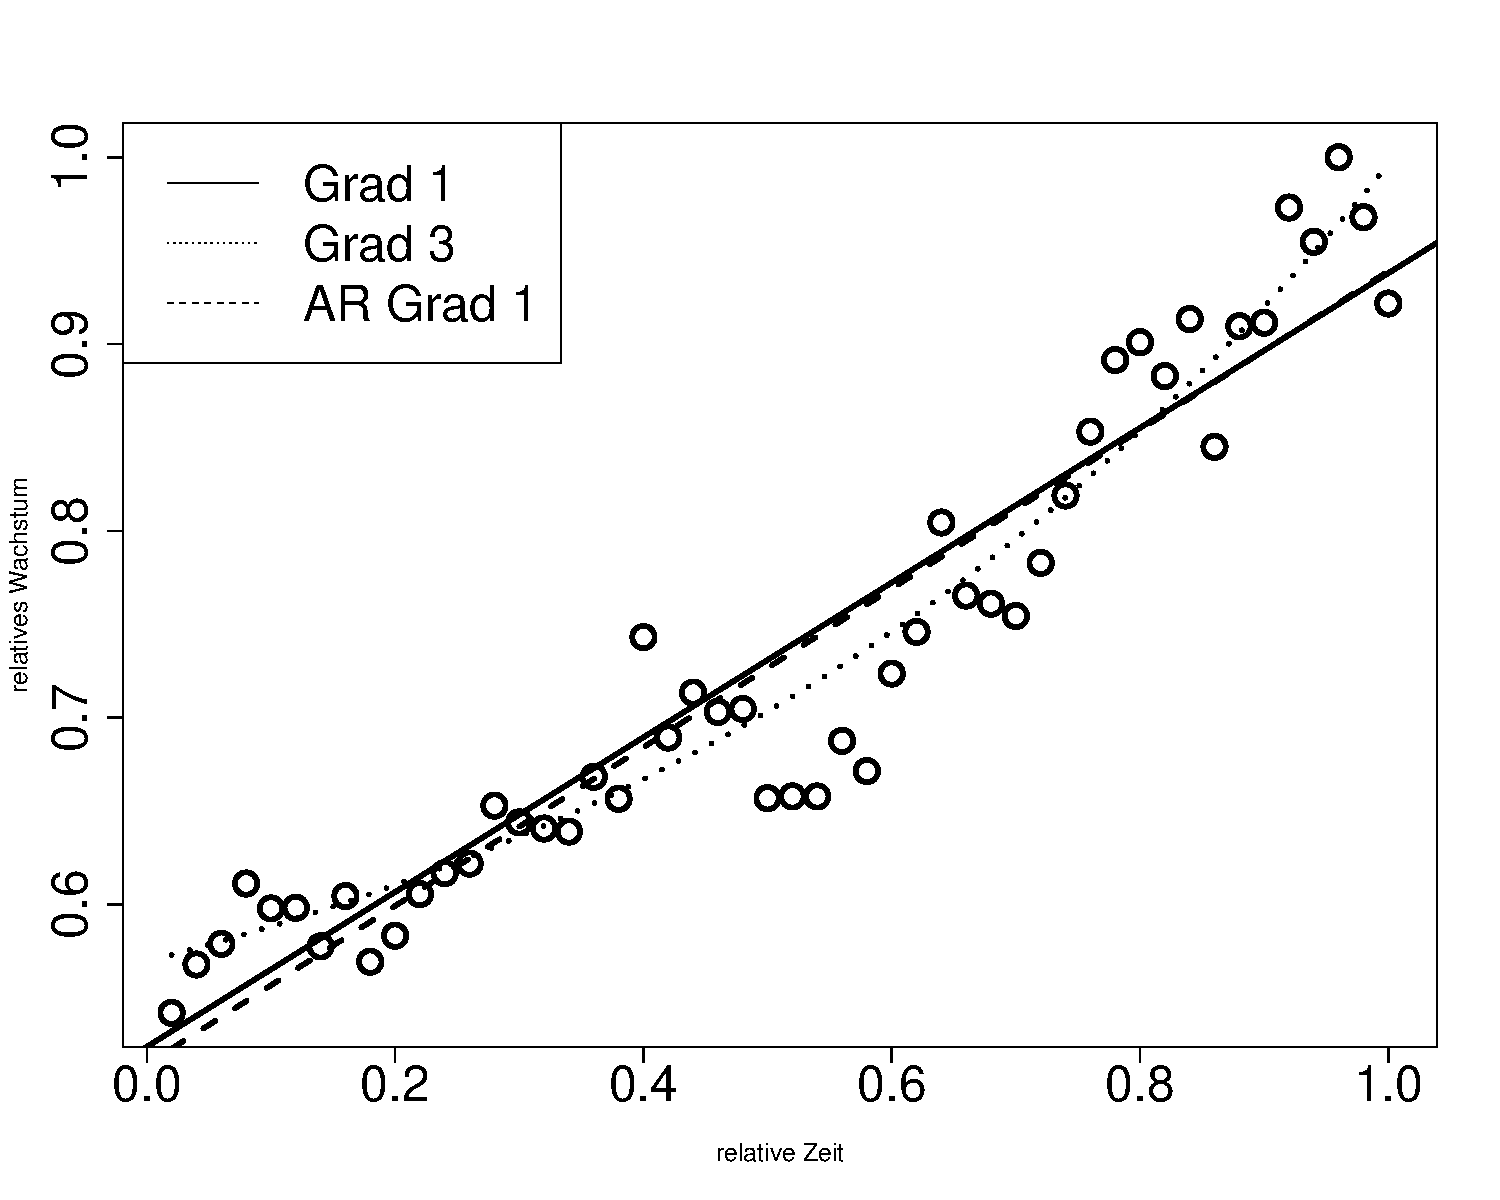
\includegraphics[width=0.5\textwidth]{Bsp-Reg-AR}
  \caption{Regression für AR(1)}
  \label{BSP-Reg-AR}
\end{figure}

Man sieht, dass ...

\end{Beispiel}




\subsection{Konfidenzbänder für AR(1)}
\label{Konfidenzbaender für AR(1)}
Im letzten Abschnitt habe ich gezeigt, dass ich einen Schätzer für $\beta$ und $\sigma^2$ bei korrelierten Daten erhalten kann, indem man beide Seiten mit der Kovarianzmatrix $\Upsilon$ multipliziert. 

Wie ich gezeigt habe ist $e^{*} = (\Upsilon^{-1/2})e \sim \mathscr{N}_0,I)$. Die Fehler dieses abgeänderten Modells sind also wieder unabhängig verteilt. Das heißt, ich kann die Ergebnisse aus Kapitel 1 anwenden und ein Konfidenzband $K^{*}$ bestimmen, sodass

\begin{align*}
\mathbb{P}(x^{*'} \beta \in K^{*}) = 1 - \alpha
\end{align*}

Da allerdings nicht $x^{*'} \beta$ interessiert, sondern $x' \beta$ muss ich noch beide Seiten der logischen Gleichheit in $\mathbb{P}()$ mit $\Upsilon^{1/2}$ multiplizieren. Auf diese Art erhalte ich dann ein Konfidenzband für unser ursprüngliches Modell \eqref{AR Modell}.

Betrachten ich nun, wie dies die Simulation aus Abschnitt \ref{Konfidenzbaenderauf auf einem Intervall für Regressionsmodell mit Polynomgestalt} beeinflusst. ich verwende die folgende Simulation, um konkret den Wert der kritischen Konstante $c$ bei abhängigen Daten zu bestimmen:

\begin{enumerate}
\item Simuliere $N \sim \mathscr{N}_0,(\Upsilon^{-1/2}X'\Upsilon^{-1/2}X)^{-1}) = (0,(X^{*'}X^{*})$ und $\hat{\sigma}/\sigma \sim \sqrt{\chi^2_v/v}$ mit $v=n-p-1$
\item Berechnung von $K_{2h}(T,(X^{*'}X^{*})^{-1},(a,b))$
\end{enumerate}

Die Berechnung von $K_{2h}(T,\cdot,(a,b))$ läuft analog zum Kapitel 1.5, da sich die Funktion $K_{2h}(T,\cdot,(a,b))$ nicht ändert.

\begin{Beispiel}
Jetzt führe ich das Beispiel aus dem ersten Kapitel fort, indem ich zu der Regression mit Grad Eins, dem Konfidenzband auf ganz $\mathbb{R}$, dem auf [min(X),max(X)] und dem auf [min(X),max(X)] für Polynome noch ein Konfidenzband auf [min(X),max(X)] für Polynome unter Berücksichtigung der AR(1)-Struktur bestimme.

\begin{figure}[H] 
  \centering
     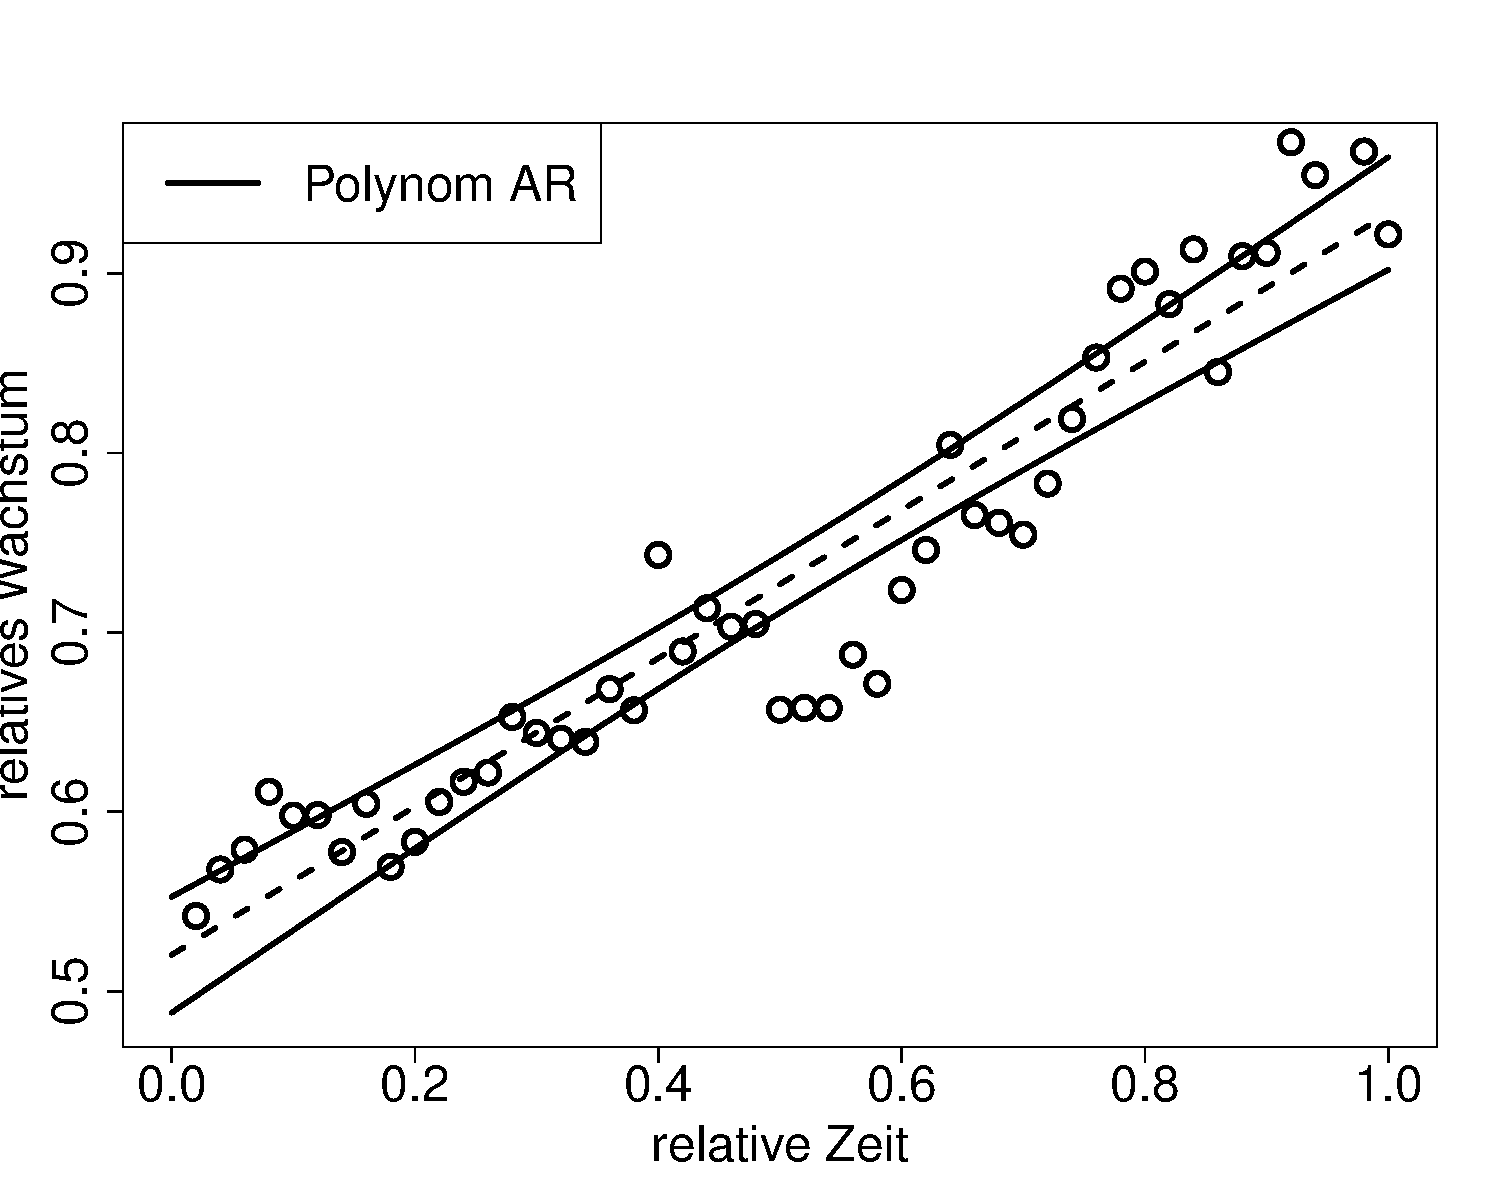
\includegraphics[width=0.5\textwidth]{Bsp-KB-poly-AR}
  \caption{Weiterführung des Beispiels durch Konfidenzband auf minamx unter Berücksichtigung von Polynomstruktur und AR(1)-Struktur}
  \label{Bsp-KB-poly-AR}
\end{figure}

Ich erhalte als kritischen Wert für das Konfidenzband auf ganz $\mathbb{R}$ \cR , für das Konfidenzband auf (min,max) \cA, für das Konfidenzband auf (min,max) für Polynome \cAP und für das Konfidenzband auf (min,max) für Polynome das die AR(1)-Struktur berücksichtigt \cAPAR . 

Da es sich um eine Simulation handelt und ich Reproduktivität gewährleisten will benutze ich die seed \seedsimulation . 

Vergleiche ich wieder die Regression mit Grad Eins und mit Grad drei erhalte ich die folgende Graphik:

\begin{figure}[H] 
  \centering
     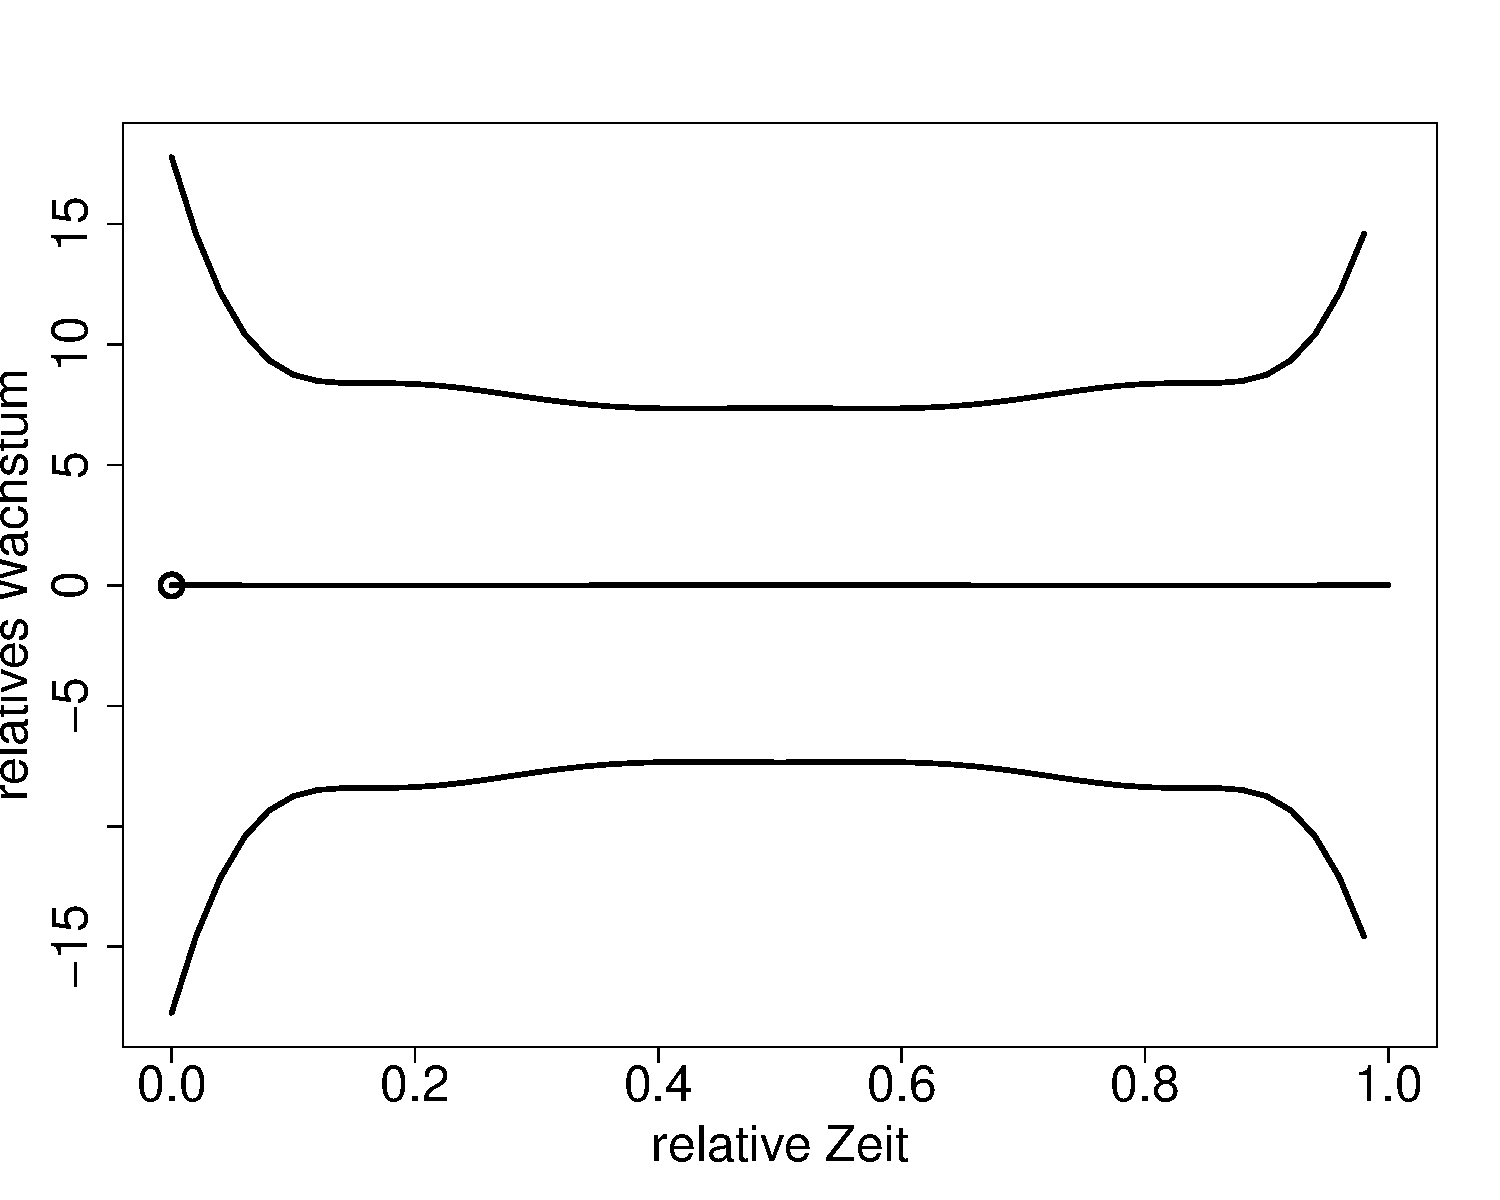
\includegraphics[width=0.5\textwidth]{Bsp-KB-poly-hetero-AR}
  \caption{Vergleich Regression Grad Eins und Grad drei unter Berücksichtigung der Polynomstruktur und AR(1)-Struktur}
  \label{Bsp-KB-poly-hetero-AR}
\end{figure}

Man sieht, dass ...

\end{Beispiel}





\newpage
\section{Datenbeschreibung und Resultate}
In diesem Kapitel beschreibe ich zuerst die Daten, die als Motivation für die bisher erklärten Methoden dienen. Danach wende ich die Methoden auf die Daten an. Zuerst vergleiche ich die Verschiedenen Methoden Konfidenzbänder zu bestimmen. Danach vergleiche ich Polynome von verschiedenem Grad. Im letzten Abschnitt vergleiche ich 10 Kilopascal (kPa) und 30 kPa Daten. Die Daten entstammen der Arbeit von \cite{Rehfeldt10}.

\subsection{Datenbeschreibung}
Die Motivation dieser Arbeit ist, wie eine Stammzelle entscheidet, zu welcher Art Gewebe sie wird. Es wird vermutet, dass Stammzellen diese Entscheidung treffen, wenn sie gerade nicht wachsen. Deshalb wurden Stammzellen auf verschiedene Untergründe gesetzt und zu jeweils bestimmten äquidistanten Zeitpunkten unter einem Mikroskop fotografiert. Danach wurde ihre Fläche bestimmt. Mit Hilfe dieser Daten habe ich eine Regression mit der Zeit als unabhängige Variable durchgeführt. Ich verwende Polynomregression, da die Ableitungen von Polynomen gut zu berechnen sind und ich so die kritischen Punkte des Regressionsgraphen einfach bestimmen kann.

Es geht darum, das beste Polynom-Modell für die Daten zu wählen. Ein Polynom-Modell ist durch den Grad des Polynoms eindeutig definiert. Das Problem ist also den besten Polynomgrad zu finden.

Um dieses Problem zu lösen, betrachtet man, ob sich die Polynome statistisch signifikant unterscheiden. Dazu schaut man die Differenz der Polynome an und berechnet für diese gleichmäßige Konfidenzbänder. Ist die Nullfuktion vollständig in diesem Konfidenzband enthalten, ist es nicht möglich, eine Aussage über den Unterschied der Modelle zu machen. Liegt die Nullfunktion allerdings nicht vollständig im Konfidenzband, ist der Unterschied signifikant.

Die konkrete Fragestellung meiner Bachelorarbeit ist, ob die Polynome, die man durch die Daten legt, sich signifikant unterscheiden.

Ich hatte Daten von Stammzellen, die auf ein Oberfläche mit einer Härte von 10 kPa oder 30 kPa gesetzt wurden. 

Es handelt sich um Daten von 53 Stammzellen bei den 30 kPa Daten und um 51 Stammzellen bei den 10 kPa Daten. Da die Stammzellen sehr verschiedene Wachstumsraten aufweisen, bilde ich den Mittelwert. 
Plotte ich nun das Mittel der relative Wachstüme gegen die Zeit entstehen folgende Graphiken. Die Berechnung für diese Graphik befindet sich in der Datei \textit{10kPa-data.R}

\begin{figure}[H] 
  \centering
     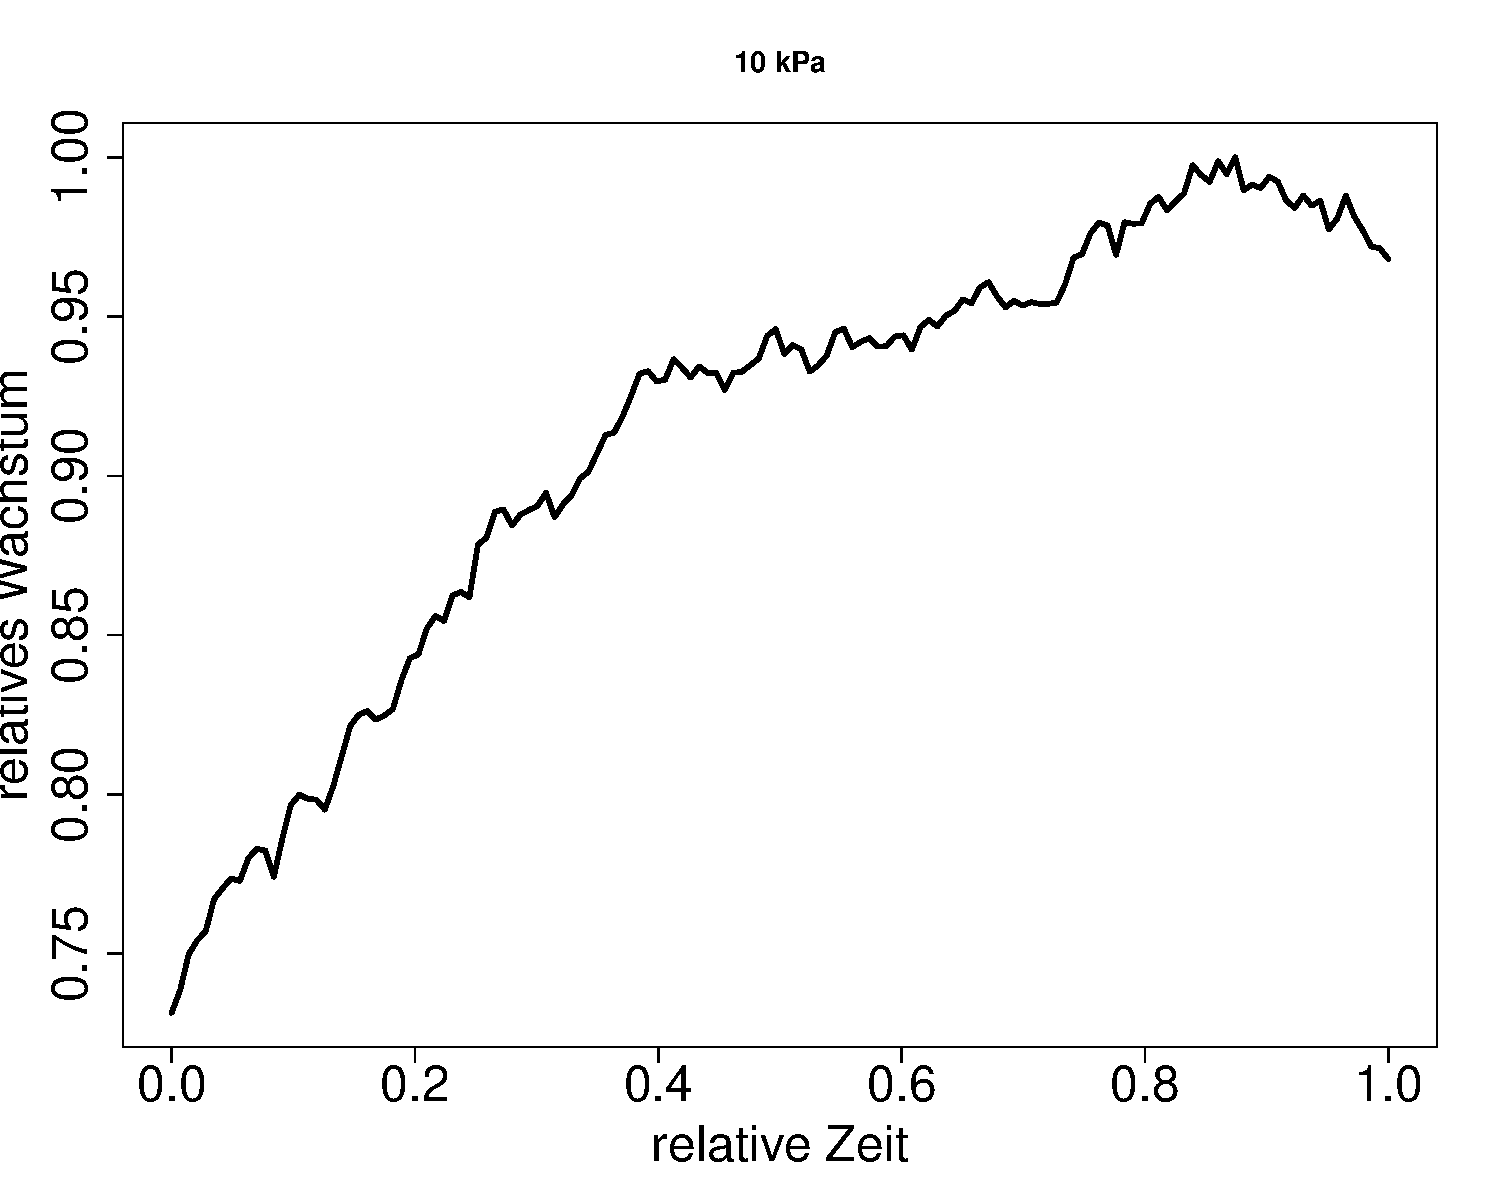
\includegraphics[width=0.5\textwidth]{10kPa-data.pdf}
  \caption{10 kPa}
  \label{10kPa-data}
\end{figure}

Man sieht, dass ...

Die Berechnung für die folgende Graphik befindet sich in der Datei \textit{30kPa-data.R}

\begin{figure}[H] 
  \centering
     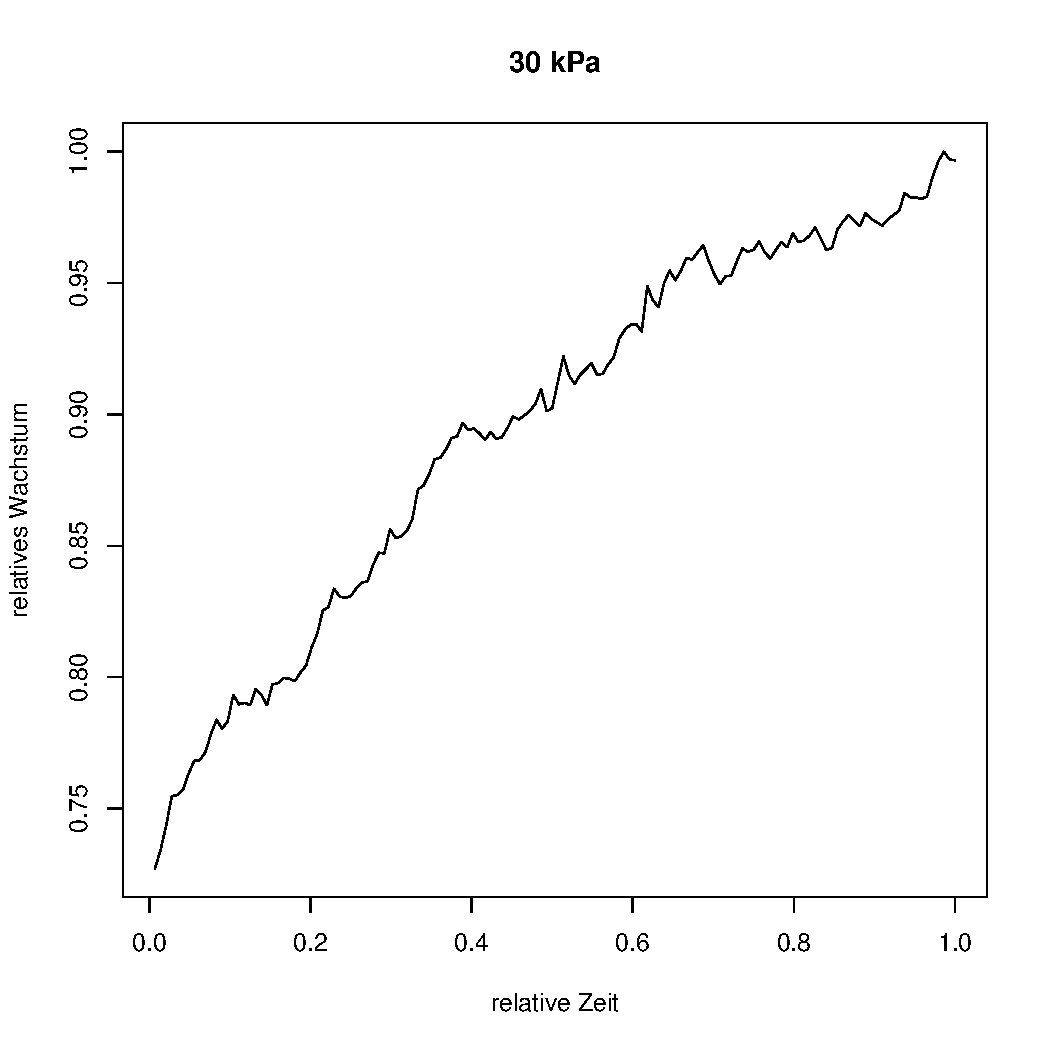
\includegraphics[width=0.5\textwidth]{30kPa-data.pdf}
  \caption{30 kPa}
  \label{30kPa-data}
\end{figure}

Man sieht, dass ...

Da es zwischen den Daten eine Autokorrelationsbeziehung der Art AR(1) gibt, muss man die Ergebnisse aus Kapitel drei anwenden.


\subsection{Vergleich verschiedener Konfidenzbänder}
Hier vergleiche ich drei Konfidenzbänder für 30kPa Daten. Das Regressionsmodell ist ein Polynom vom Grad vier mit OLS. Das Konfidenzband auf ganz $R$ ist ..., das Konfidenzband auf $(min,max)$ ist ... und das die Polynomstruktur berücksichtigt ist ... . 

Die Berechnung für diese Graphik befindet sich in der Datei \textit{30kPa-method.R}

\begin{figure}[H] 
  \centering
     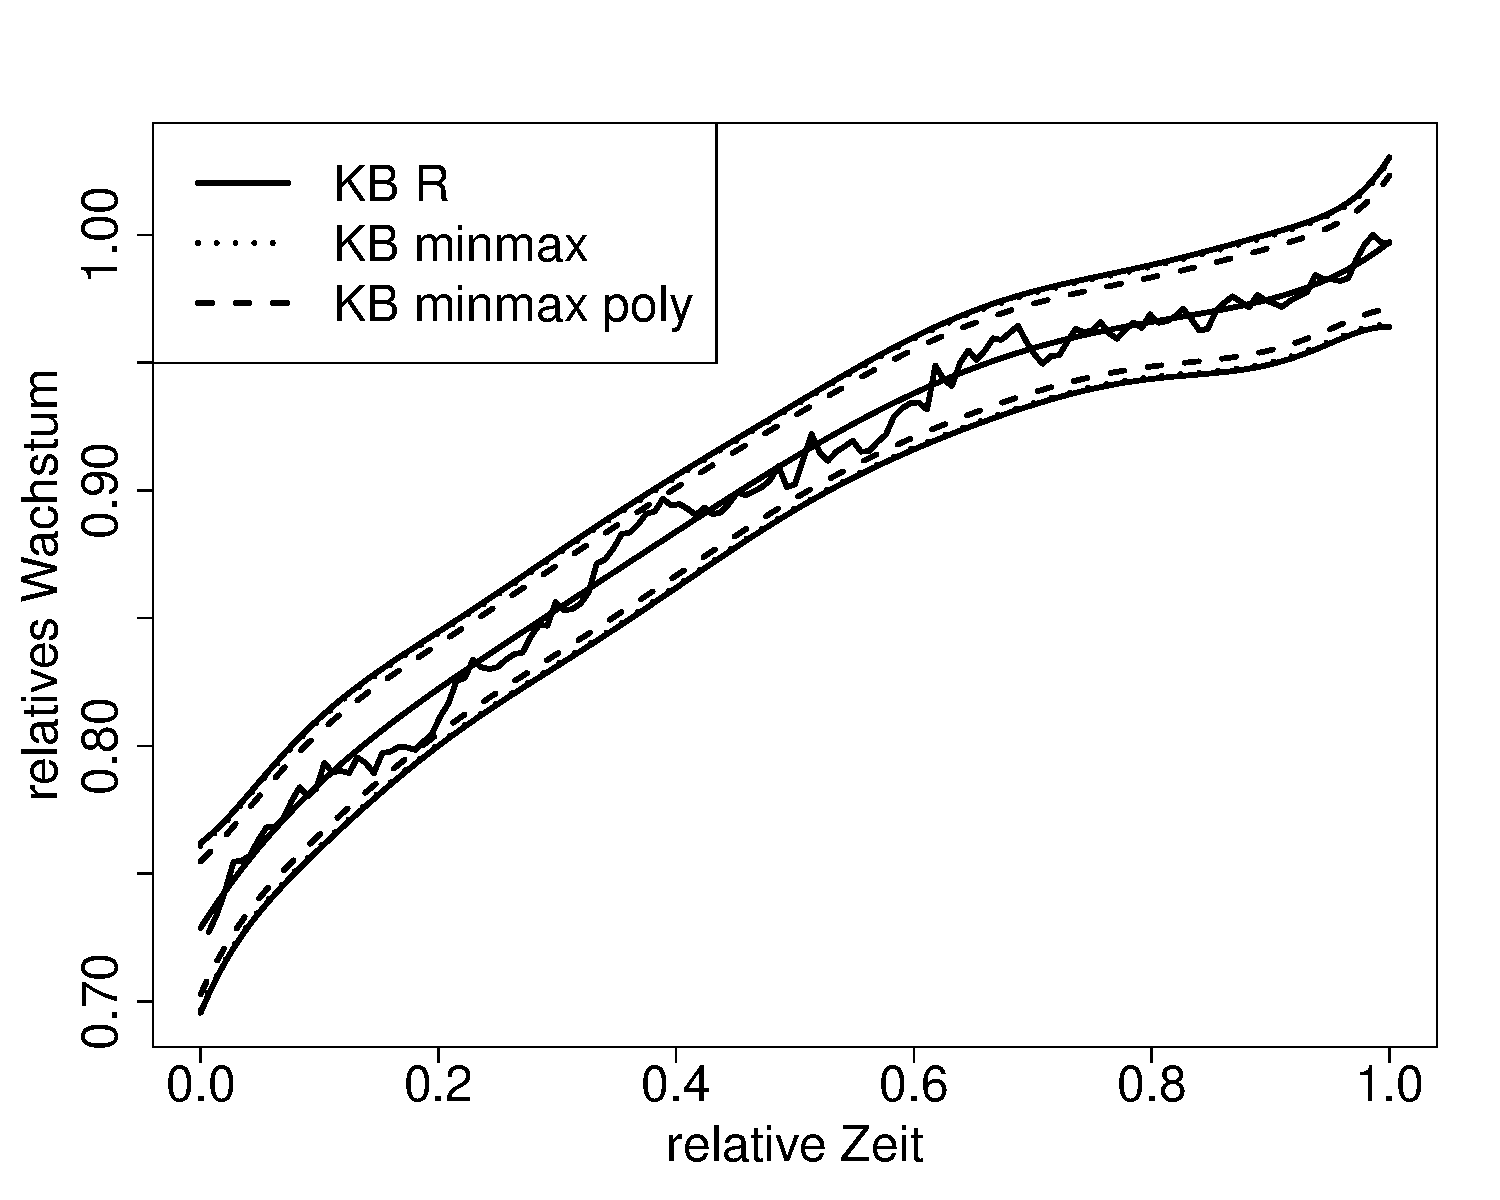
\includegraphics[width=0.5\textwidth]{30kPa-method.pdf}
  \caption{Vergleich von Konfidenzbändern 30 kPa}
  \label{fig:3}
\end{figure}

Man sieht, dass  das Konfidenzband auf $(min,max)$, das die Polynomstruktur berücksichtigt, deutlich schmaler ist. Dies wird auch an der kleineren kritischen Konstante c von ... im Gegensatz zu ... deutlich.

Graphik Vergleich aller drei KBer für 10 kPa Daten

Die Berechnung für diese Graphik befindet sich in der Datei \textit{10kPa-method.R}

\begin{figure}[H] 
  \centering
     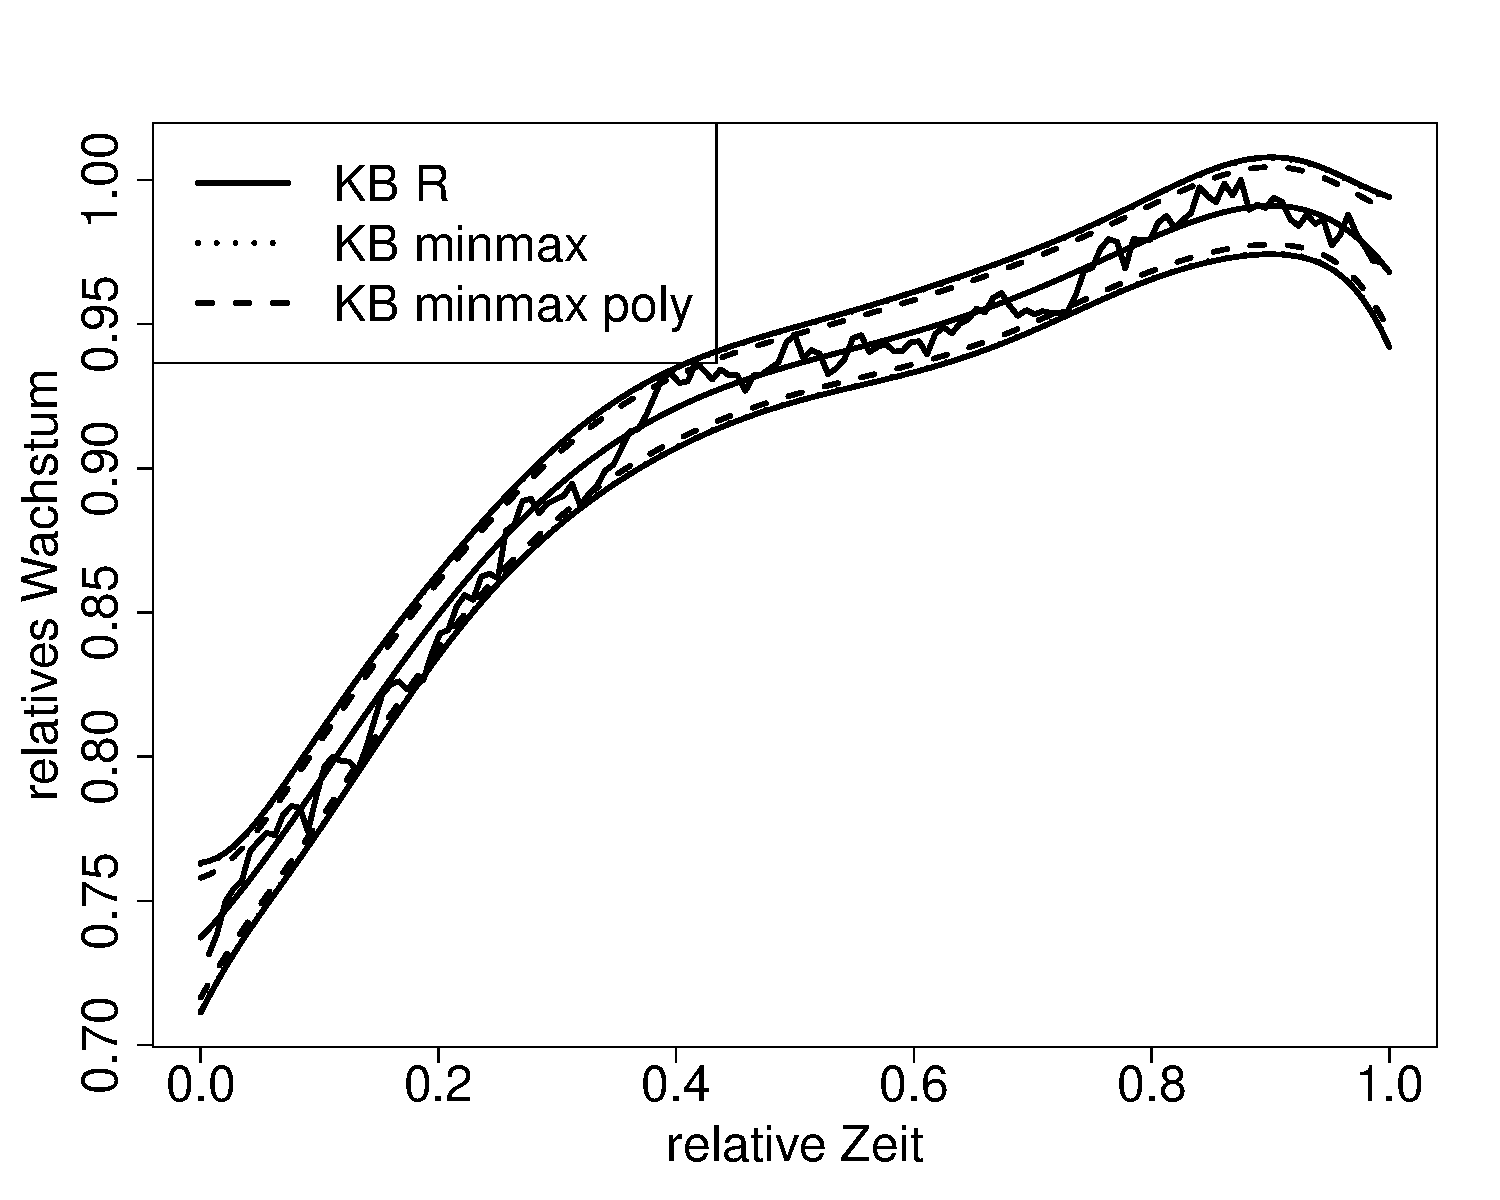
\includegraphics[width=0.5\textwidth]{10kPa-method.pdf}
  \caption{Vergleich von Konfidenzbändern 10 kPa}
  \label{fig:4}
\end{figure}



%\subsection{Welches Modell ist das richtige ?}
%In diesem Abschnitt schaue ich, ob die verschiedenen Modelle um Regression durchzuführen sich signifikant unterscheiden.
%
%Graphik ols, fgls, ar1 für 10 kPa :
%
%\begin{figure}[H] 
%  \centering
%     \includegraphics[width=0.5\textwidth]{10kPa-model.pdf}
%  \caption{Vergleich von Regressionsmodellen}
%  \label{fig:5}
%\end{figure}
%
%3er Graphik fgls vs ols, ols vs ar1, ar1 vs ols für 10 kPa :
%
%\begin{figure}[H] 
%  \centering
%     \includegraphics[width=0.5\textwidth]{10kPa-model-KB.pdf}
%  \caption{Vergleich von Regressionsmodellen}
%  \label{fig:6}
%\end{figure}
%
%Graphik ols, fgls, ar1 für 30 kPa :
%
%\begin{figure}[H] 
%  \centering
%     \includegraphics[width=0.5\textwidth]{30kPa-model.pdf}
%  \caption{Vergleich von Regressionsmodellen}
%  \label{fig:7}
%\end{figure}
%
%3er Graphik fgls vs ols, ols vs ar1, ar1 vs ols für 30 kPa :
%
%\begin{figure}[H] 
%  \centering
%     \includegraphics[width=0.5\textwidth]{30kPa-model-KB.pdf}
%  \caption{Vergleich von Regressionsmodellen}
%  \label{fig:8}
%\end{figure}
%




\subsection{Vergleich von Polynomen mit verschiedenem Grad}
In diesem Abschnitt vergleiche ich Polynomregression mit verschiedenen Polynomgraden.

Graphik Polynome vom Grad 4,5,6 für 30 kPa Daten :

Die Berechnung für diese Graphik befindet sich in der Datei \textit{30kPa-poly.R}

\begin{figure}[H] 
  \centering
     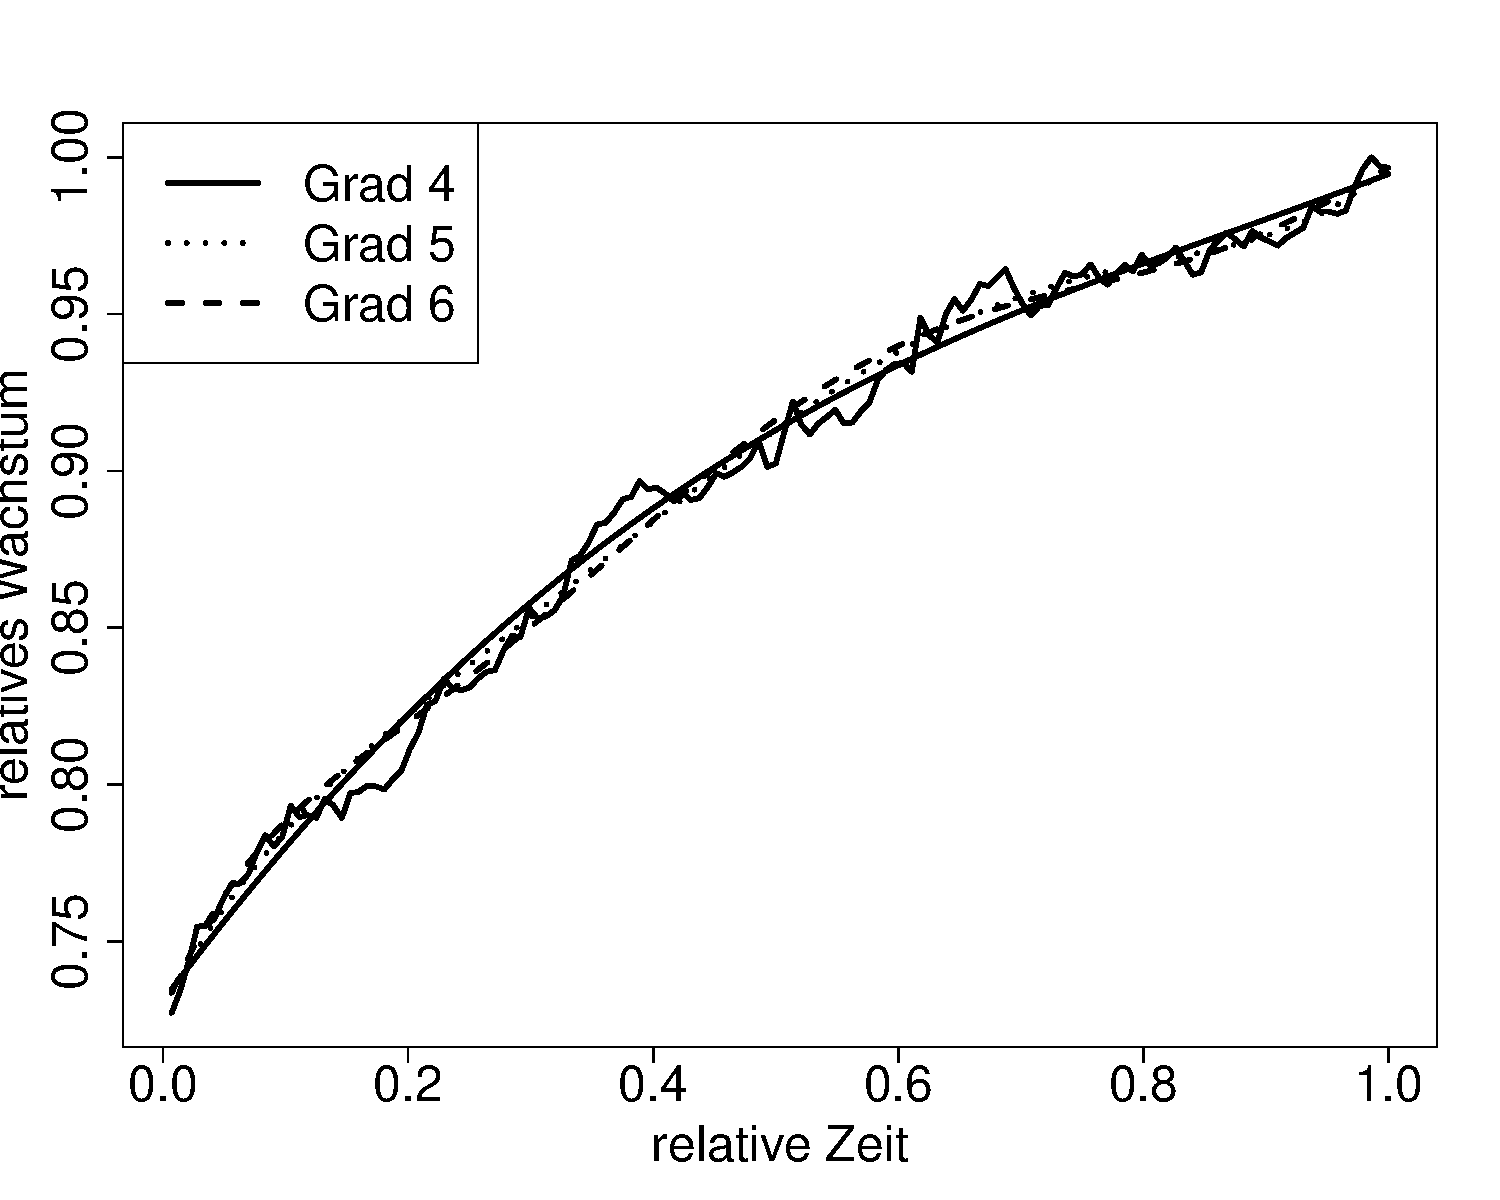
\includegraphics[width=0.5\textwidth]{30kPa-poly.pdf}
  \caption{Vergleich von Regressionsmodellen}
  \label{fig:11}
\end{figure}

3er Graphik Vergleich von Modellen poly 4,5,6 30 kPa

Die Berechnung für diese Graphik befindet sich in der Datei \textit{30kPa-poly-KB.R}

\begin{figure}[H] 
  \centering
     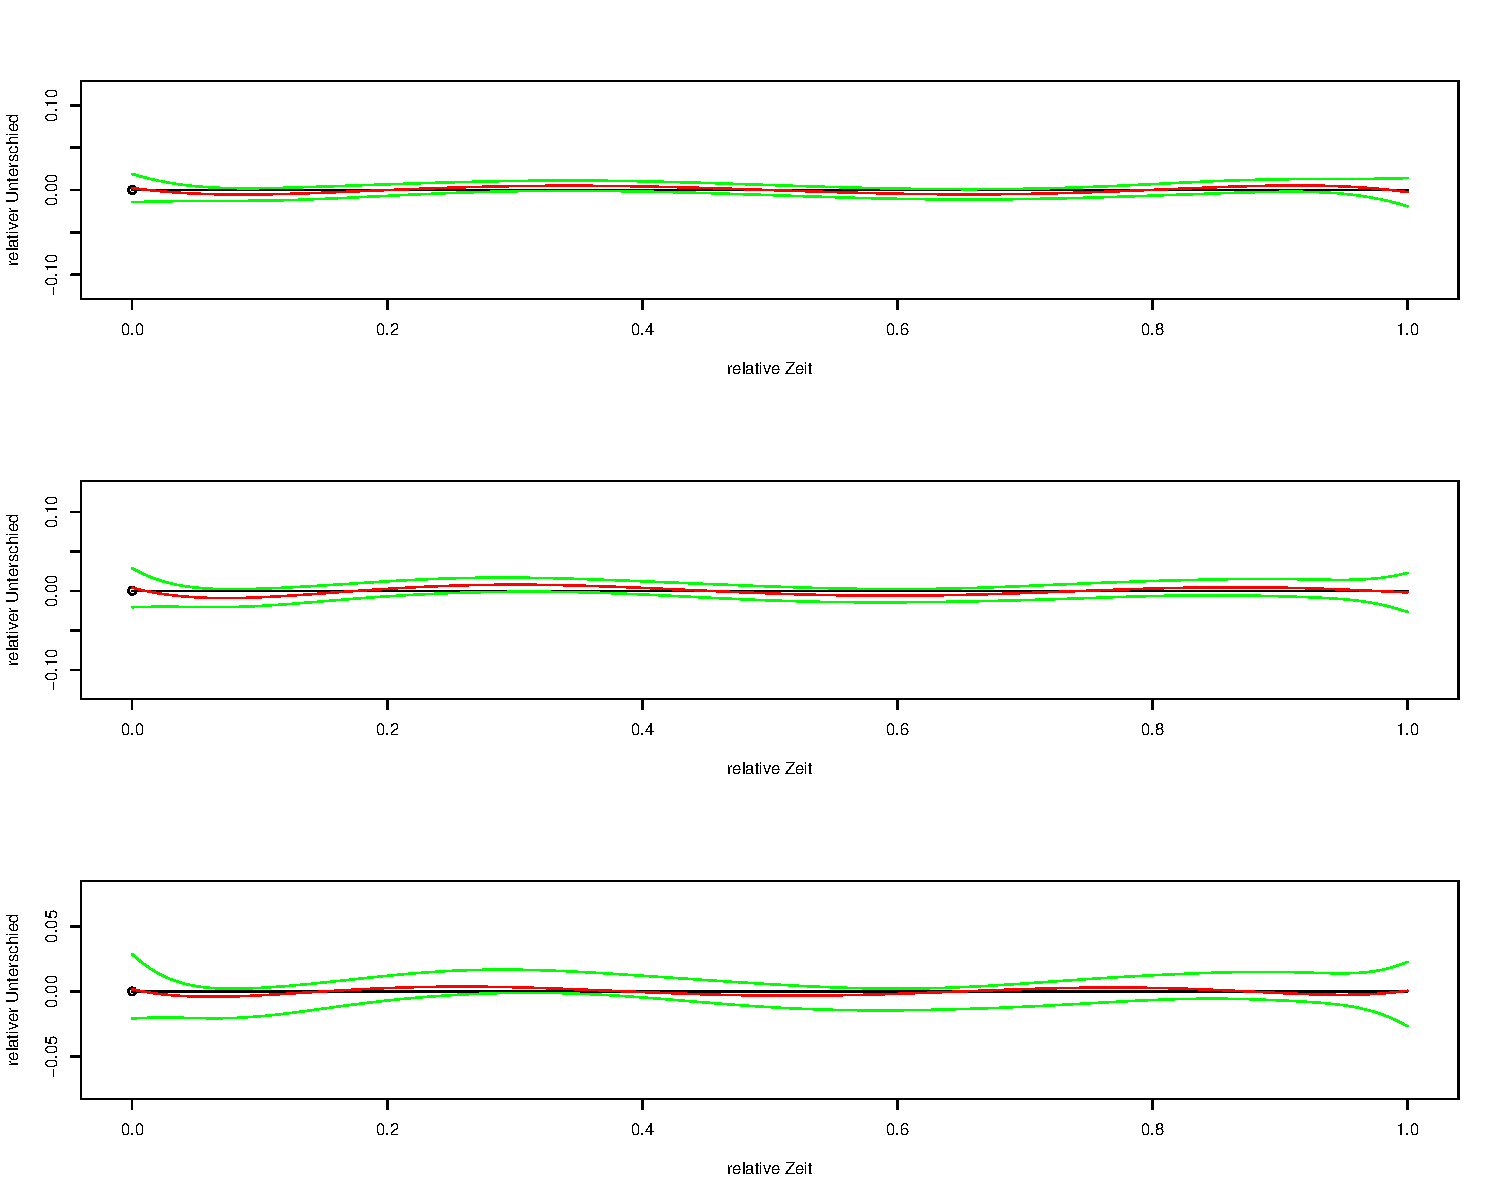
\includegraphics[width=0.5\textwidth]{30kPa-poly-KB.pdf}
  \caption{Vergleich von Regressionsmodellen}
  \label{fig:12}
\end{figure}

Graphik Polynome vom Grad 4,5,6 für 10 kPa Daten

Die Berechnung für diese Graphik befindet sich in der Datei \textit{10kPa-poly.R}

\begin{figure}[H] 
  \centering
     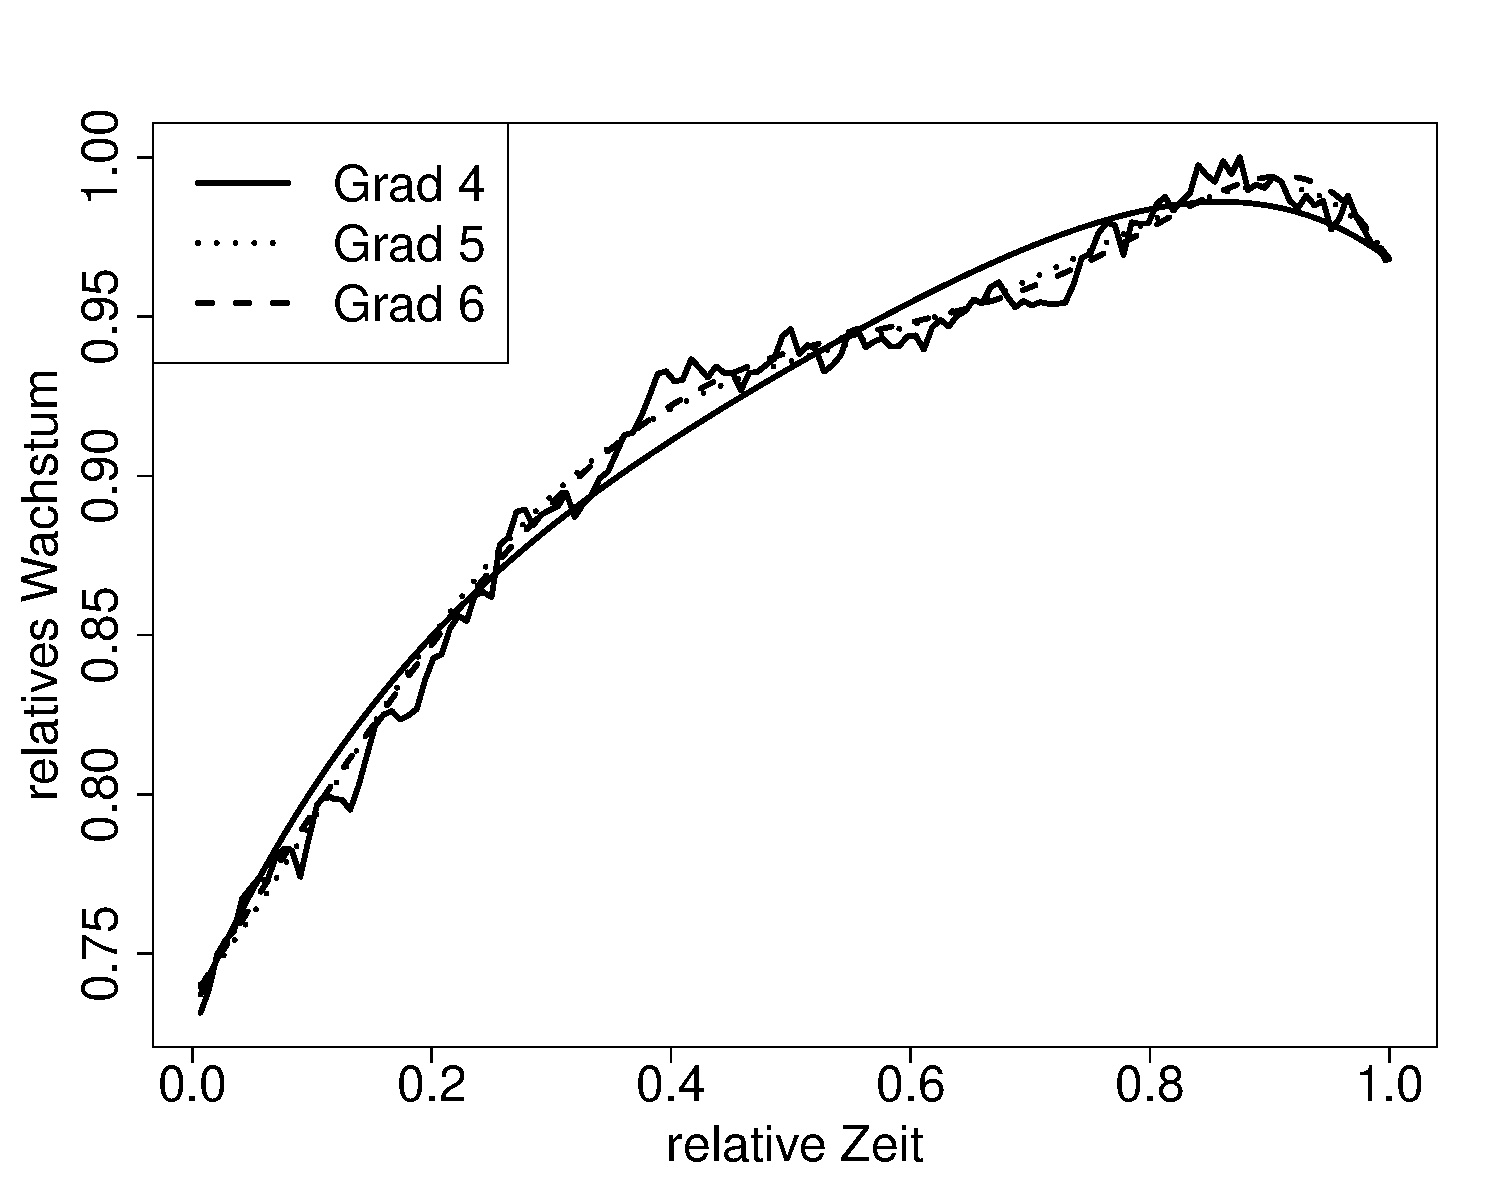
\includegraphics[width=0.5\textwidth]{10kPa-poly.pdf}
  \caption{Vergleich von Regressionsmodellen}
  \label{fig:13}
\end{figure}

3er Graphik Vergleich von Modellen poly 4,5,6 30 kPa

Die Berechnung für diese Graphik befindet sich in der Datei \textit{10kPa-poly-KB.R}

\begin{figure}[H] 
  \centering
     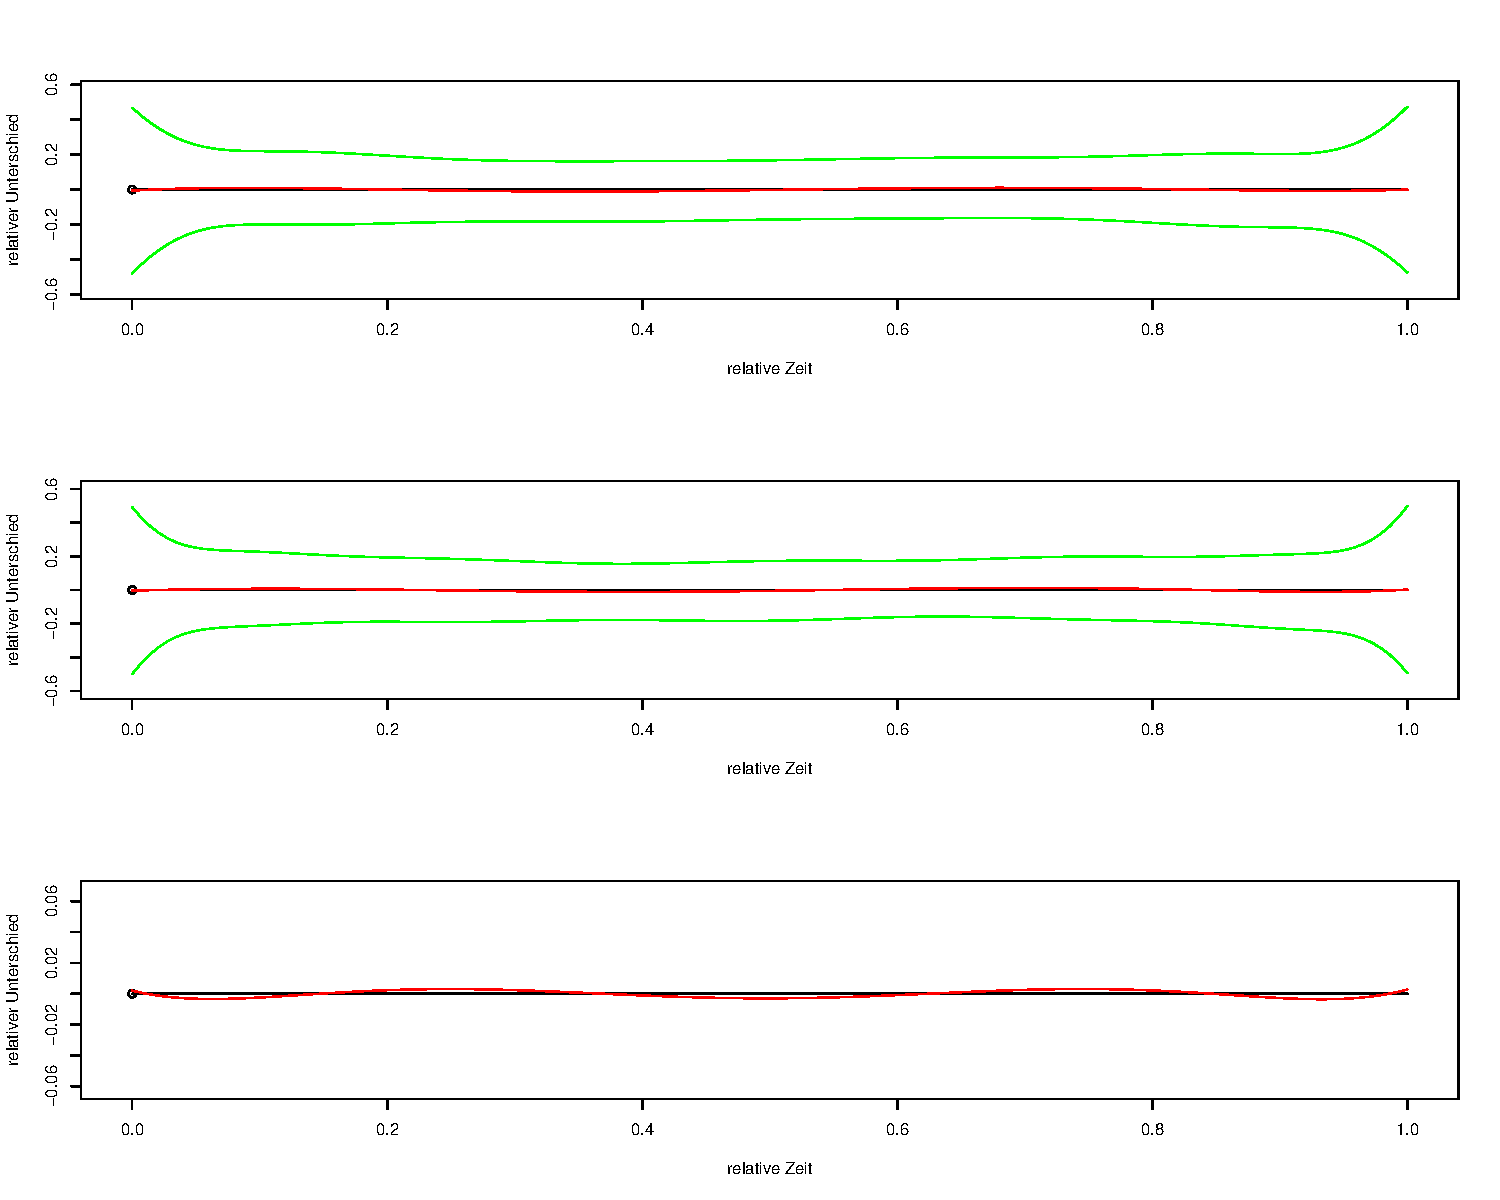
\includegraphics[width=0.5\textwidth]{10kPa-poly-KB.pdf}
  \caption{Vergleich von Regressionsmodellen}
  \label{fig:14}
\end{figure}



\subsection{Vergleich von 10 kPa und 30 kPa Daten}
In meinem nächsten Plot vergleiche ich 10 kPa mit 30 kPa OLS. Dazu plotte ich zuerst die beiden Daten mit AR(1) Regressionsmodellen in eine Graphik.

Die Berechnung für diese Graphik befindet sich in der Datei \textit{Vergleich-10vs30-poly5.R}

\begin{figure}[H] 
  \centering
     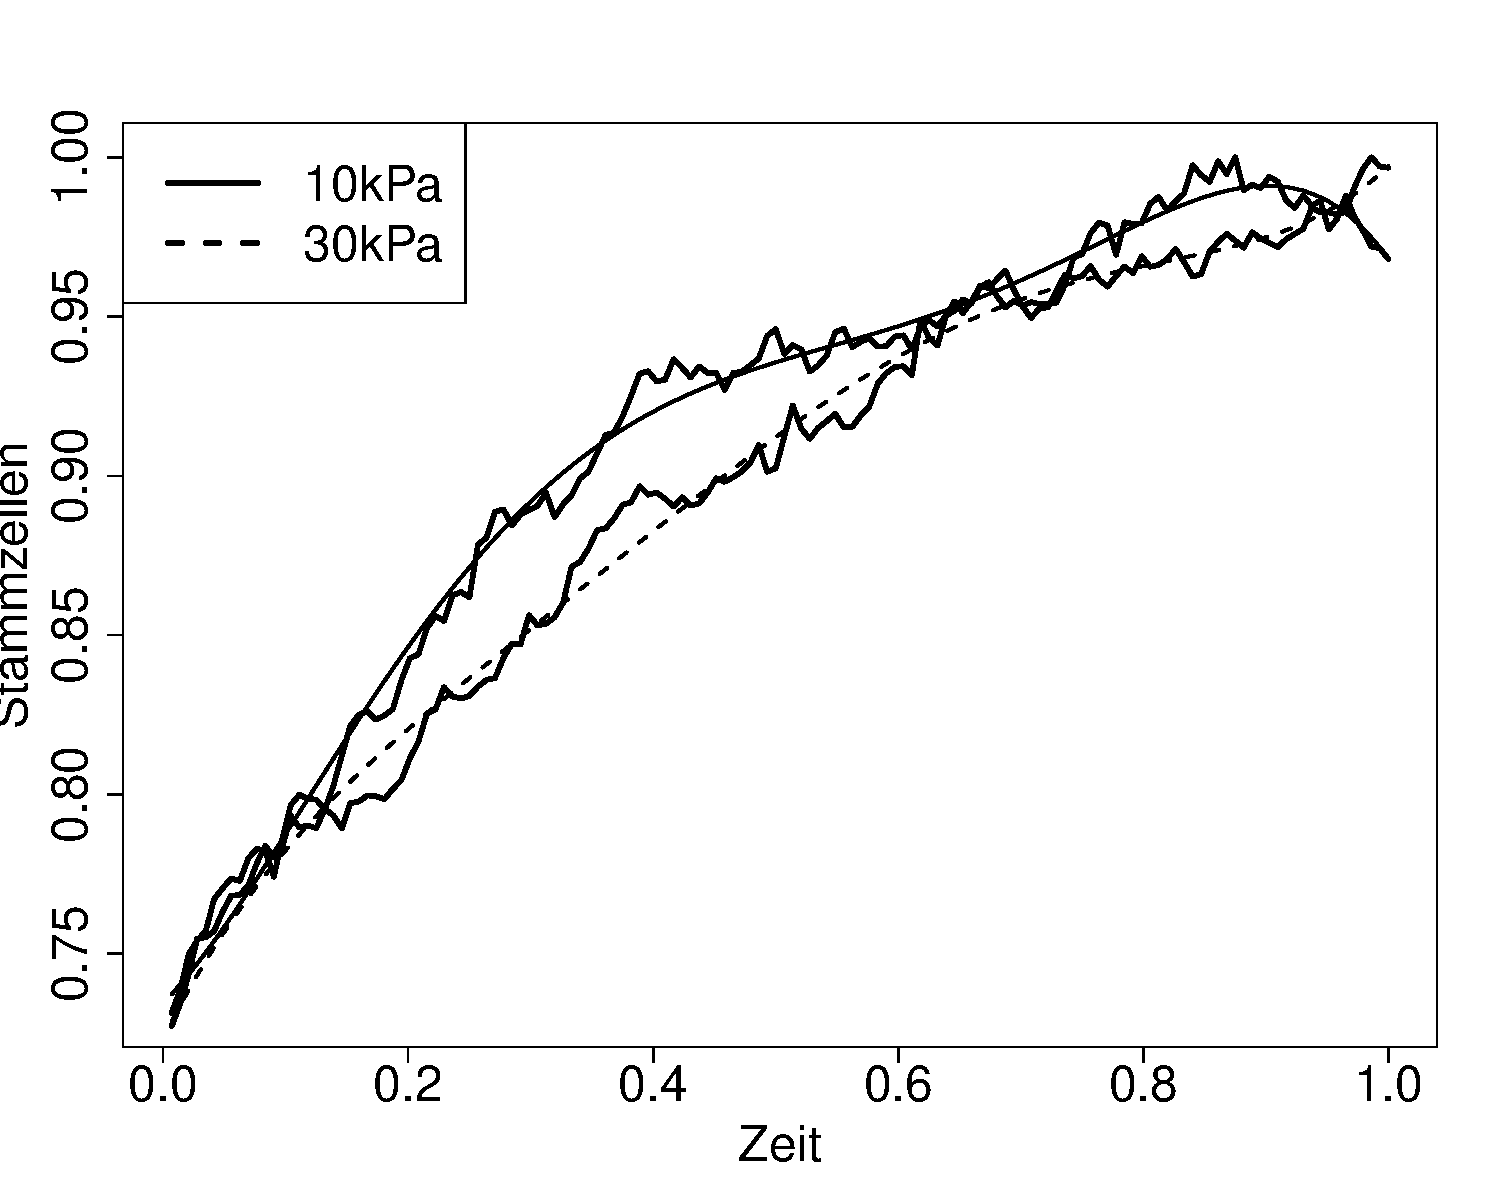
\includegraphics[width=0.5\textwidth]{Vergleich-10vs30-poly5}
  \caption{Vergleich von Regressionsmodellen}
  \label{fig:9}
\end{figure}


Als nächstes plotte ich die Differenz mit Konfidenzband in einer Graphik

Die Berechnung für diese Graphik befindet sich in der Datei \textit{Vergleich-10vs30-poly5-KB.R}

\begin{figure}[H] 
  \centering
     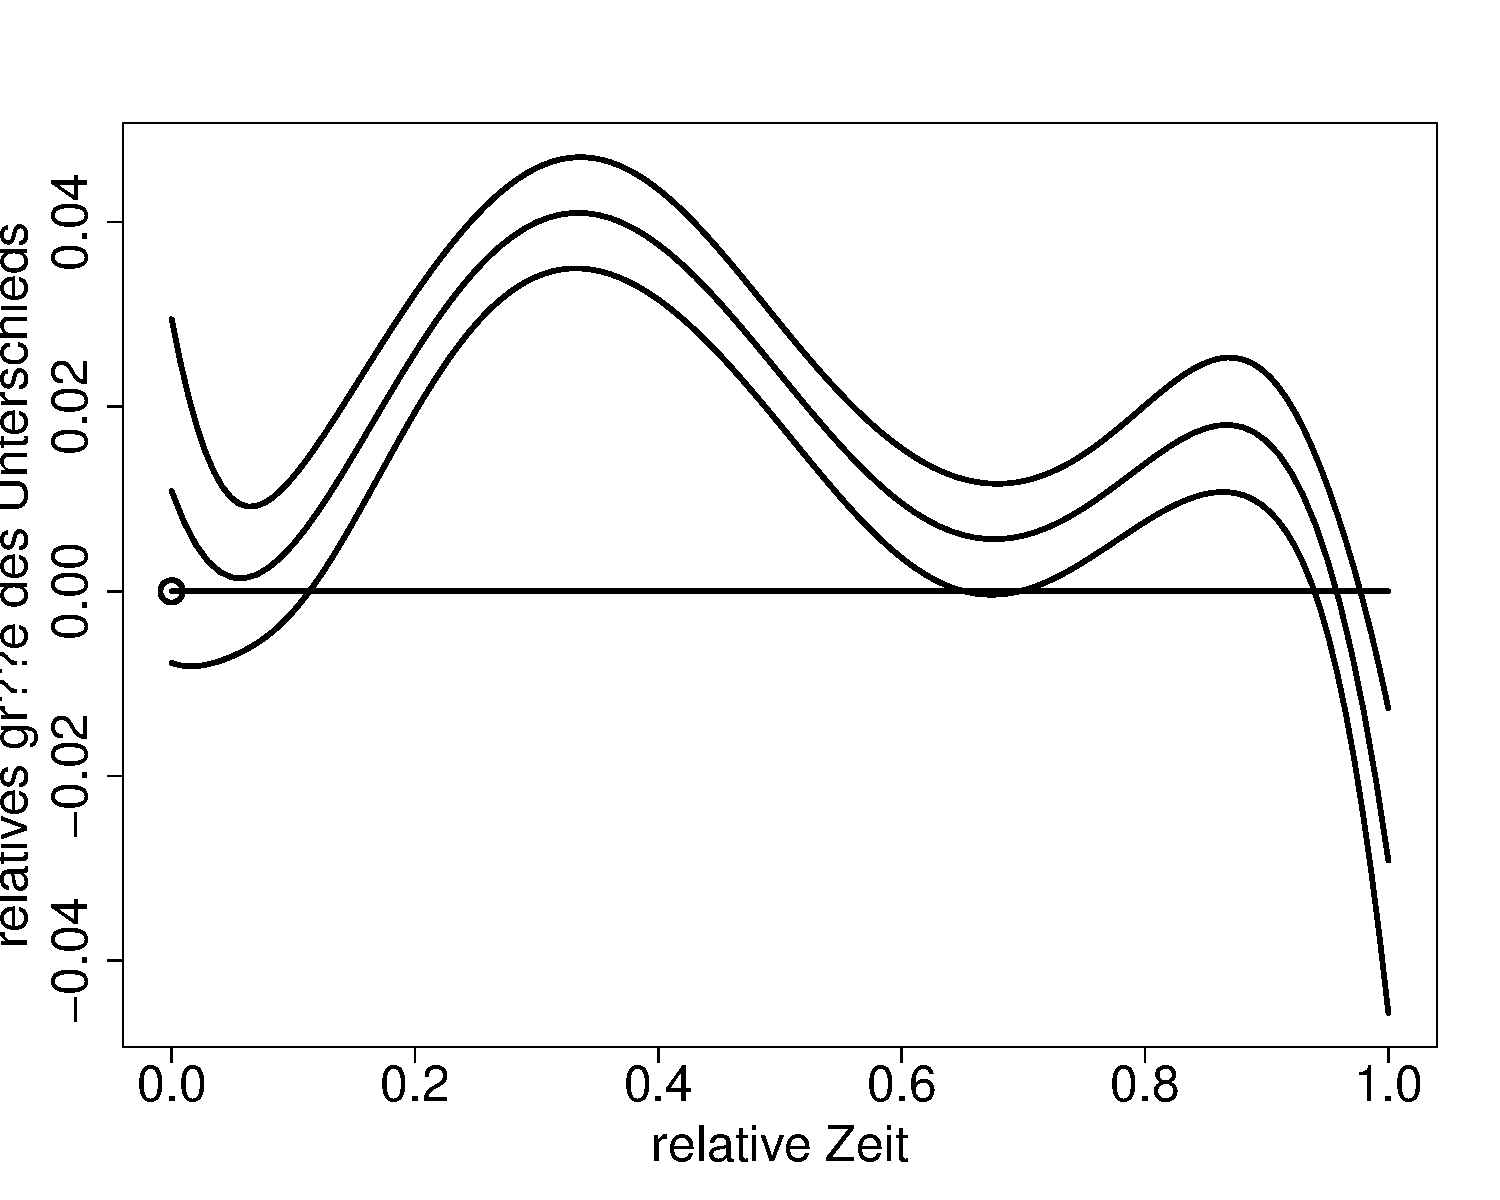
\includegraphics[width=0.5\textwidth]{Vergleich-10vs30kPa-poly5-KB}
  \caption{Vergleich von Regressionsmodellen}
  \label{fig:10}
\end{figure}

Man sieht, dass die Nullfunktion nicht komplett im Konfidenzband enthalten ist. Dies bedeutet, dass ...


\subsection{Teil eines Regressionsmodells überprüfen}
Die Berechnungen für diesen Abschnitt befinden sich in der Datei \textit{05-xxkPa-pruefen}. Dabei ist \textit{xx} entweder 10 oder 30 und die Datei ist im jeweiligen Unterordner zu finden.

In diesem Abschnitt wird getestet, ob bei einem Regressionsmodell vom Grad 5 die erste Komponente nicht signifikant, beziehungsweise ob bei einem Regressionsmodell vom Grad 6 die erste oder sogar die ersten beiden Komponenten gleich Null sind. Dazu verwende ich die Methode aus Abschnitt \ref{Teil eines Regressionsmodells überpruefen, wenn das Modell Polynomgestalt hat}.

Zuerst der Grad 5:

\begin{figure}[H] 
  \centering
     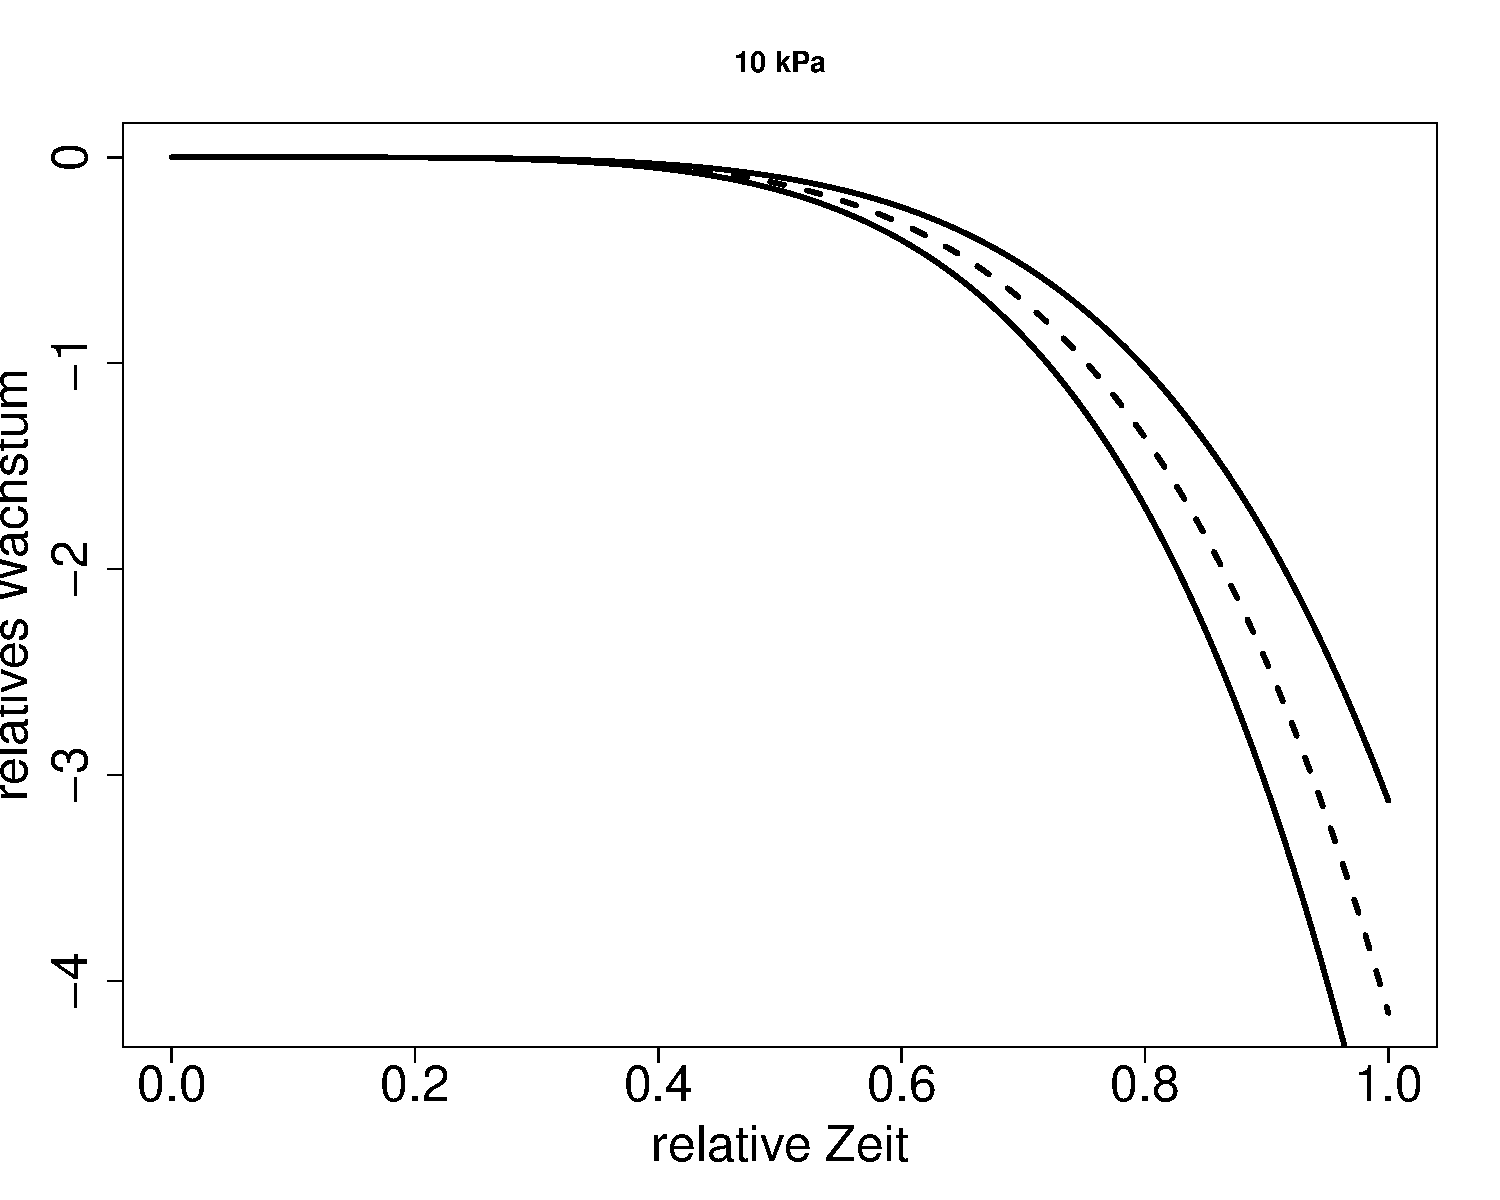
\includegraphics[width=0.5\textwidth]{10kPa-Grad-5-KB}
  \caption{10kPa Grad 5}
  \label{10kPa Grad 5}
\end{figure}

\begin{figure}[H] 
  \centering
     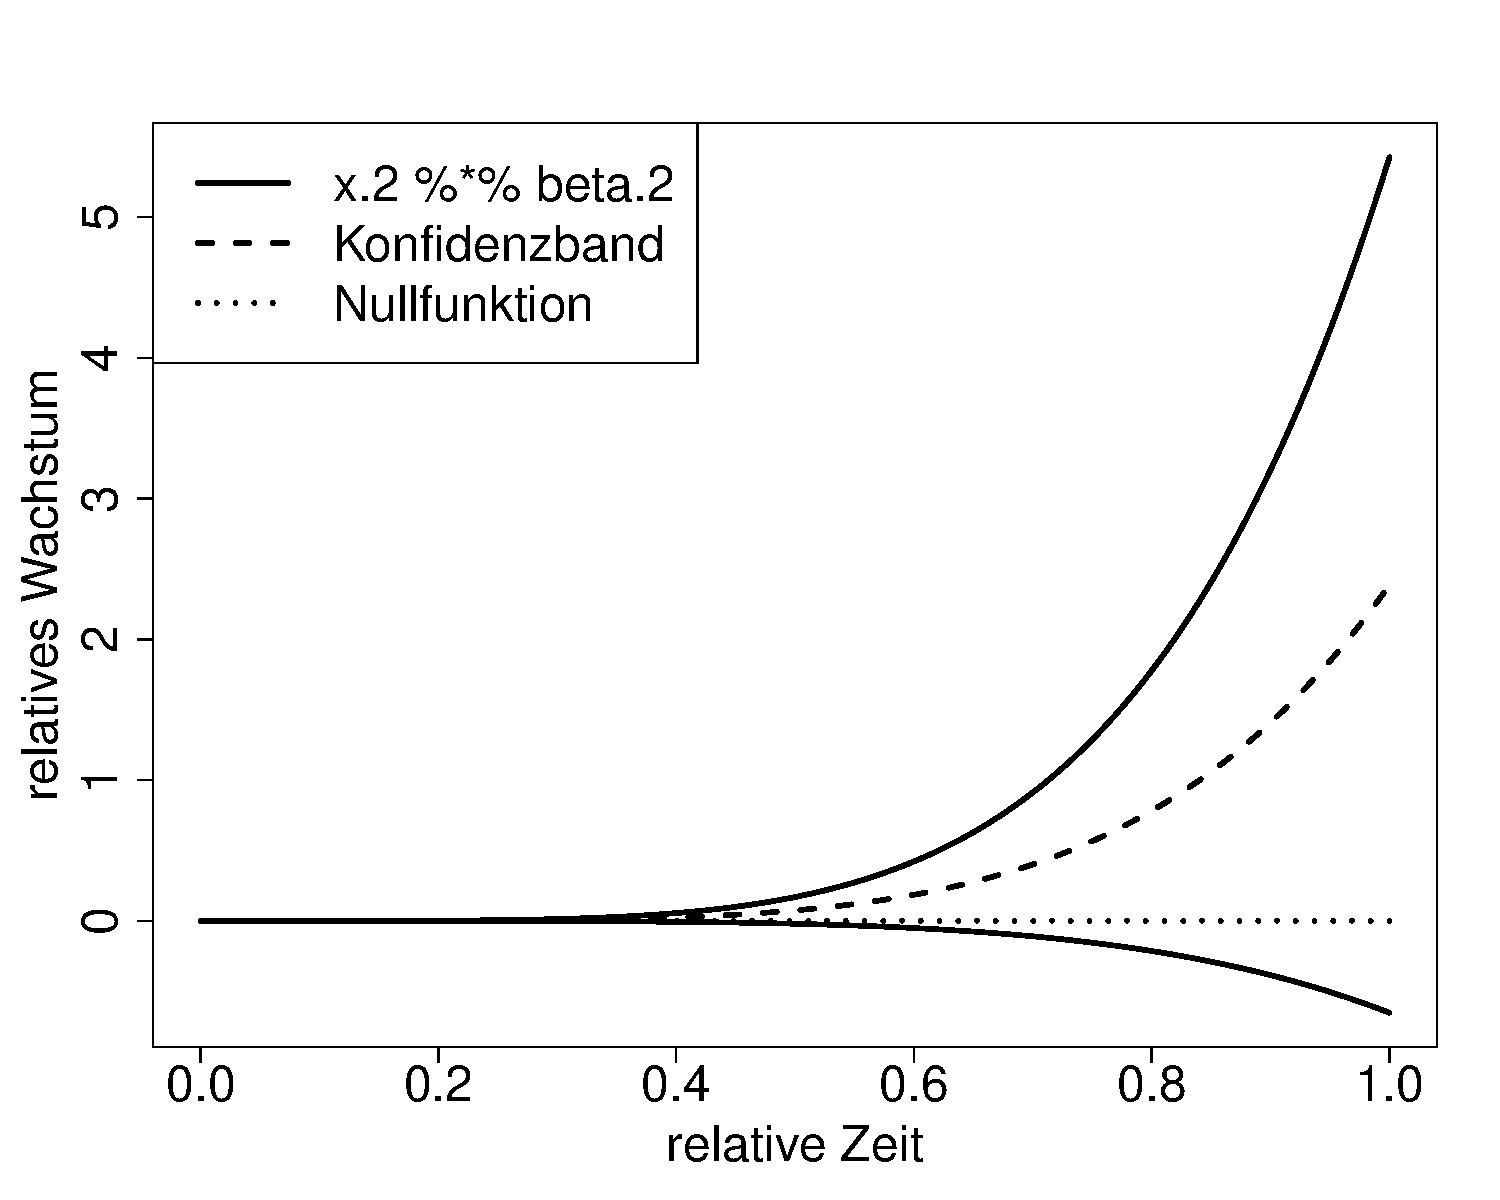
\includegraphics[width=0.5\textwidth]{30kPa-Grad-5-KB}
  \caption{30kPa Grad 5}
  \label{30kPa Grad 5}
\end{figure}

Dann der Grad 6 für 30kPa:

\begin{figure}[H] 
  \centering
     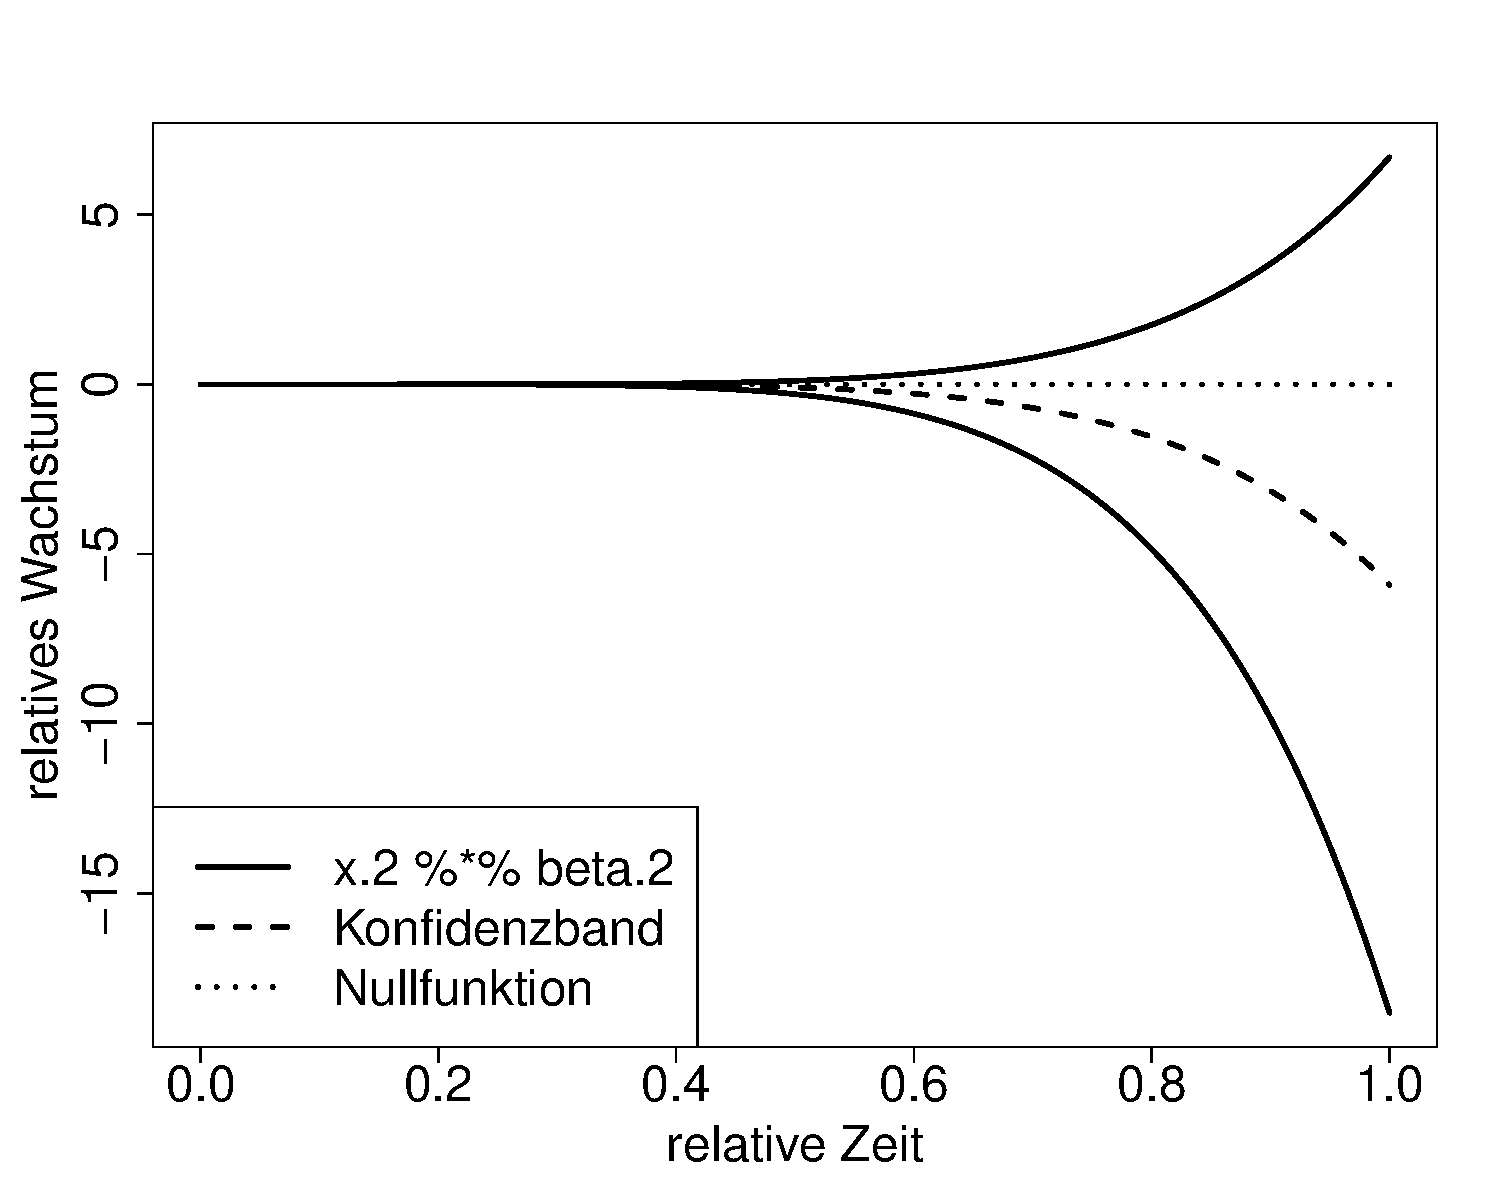
\includegraphics[width=0.5\textwidth]{30kPa-Grad-6-1-KB}
  \caption{30kPa Grad 6.1}
  \label{30kPa Grad 6.1}
\end{figure}

\begin{figure}[H] 
  \centering
     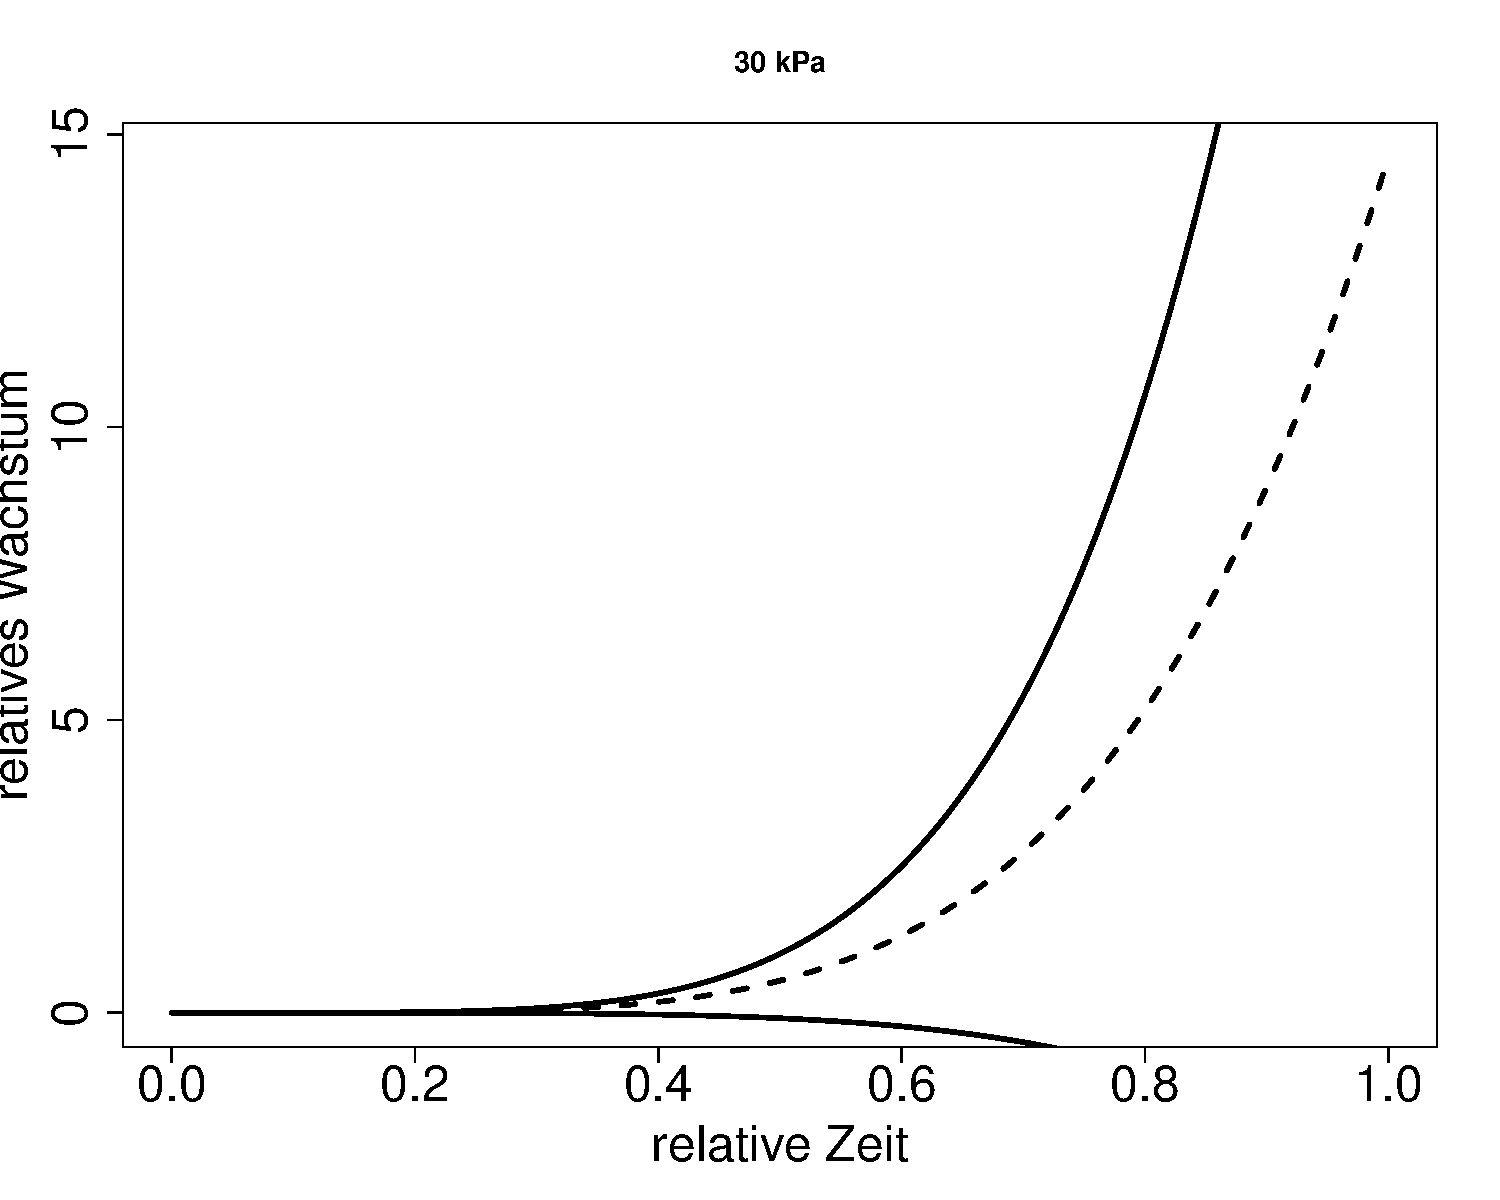
\includegraphics[width=0.5\textwidth]{30kPa-Grad-6-2-KB}
  \caption{30kPa Grad 6.2}
  \label{30kPa Grad 6.2}
\end{figure}

Zum Schluss der Grad 6 für 10kPa:

\begin{figure}[H] 
  \centering
     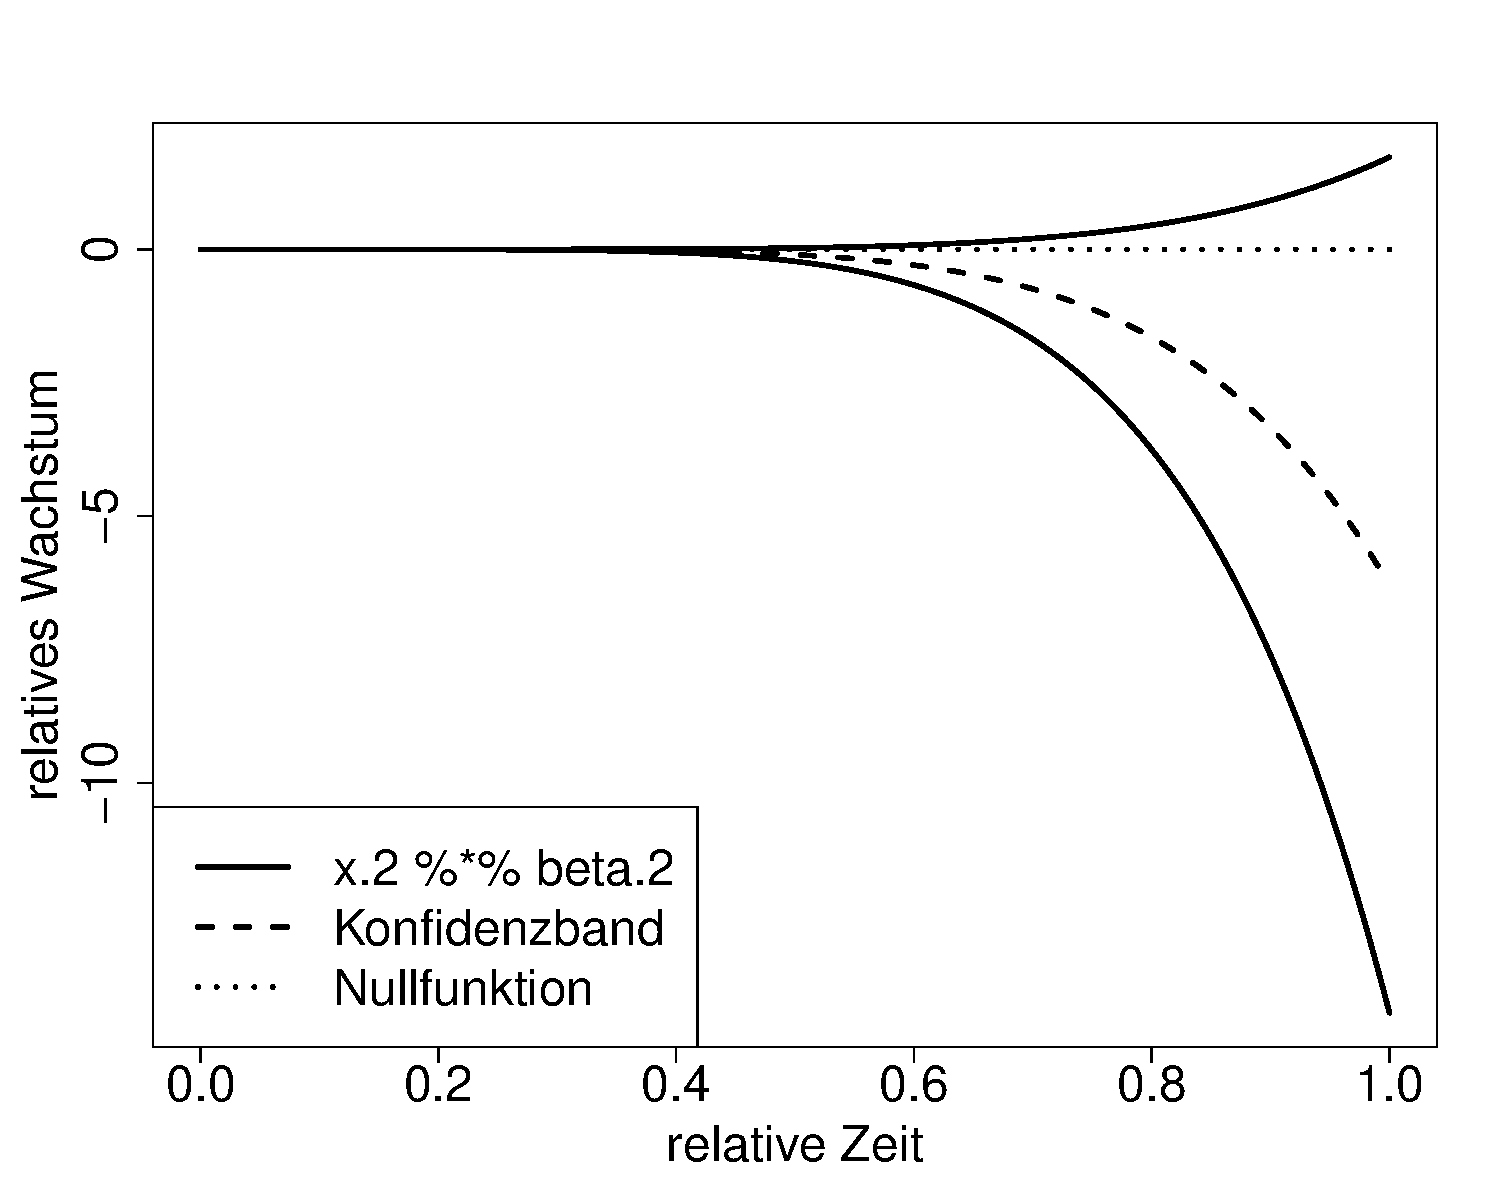
\includegraphics[width=0.5\textwidth]{10kPa-Grad-6-1-KB}
  \caption{10kPa Grad 6.1}
  \label{10kPa Grad 6.1}
\end{figure}

\begin{figure}[H] 
  \centering
     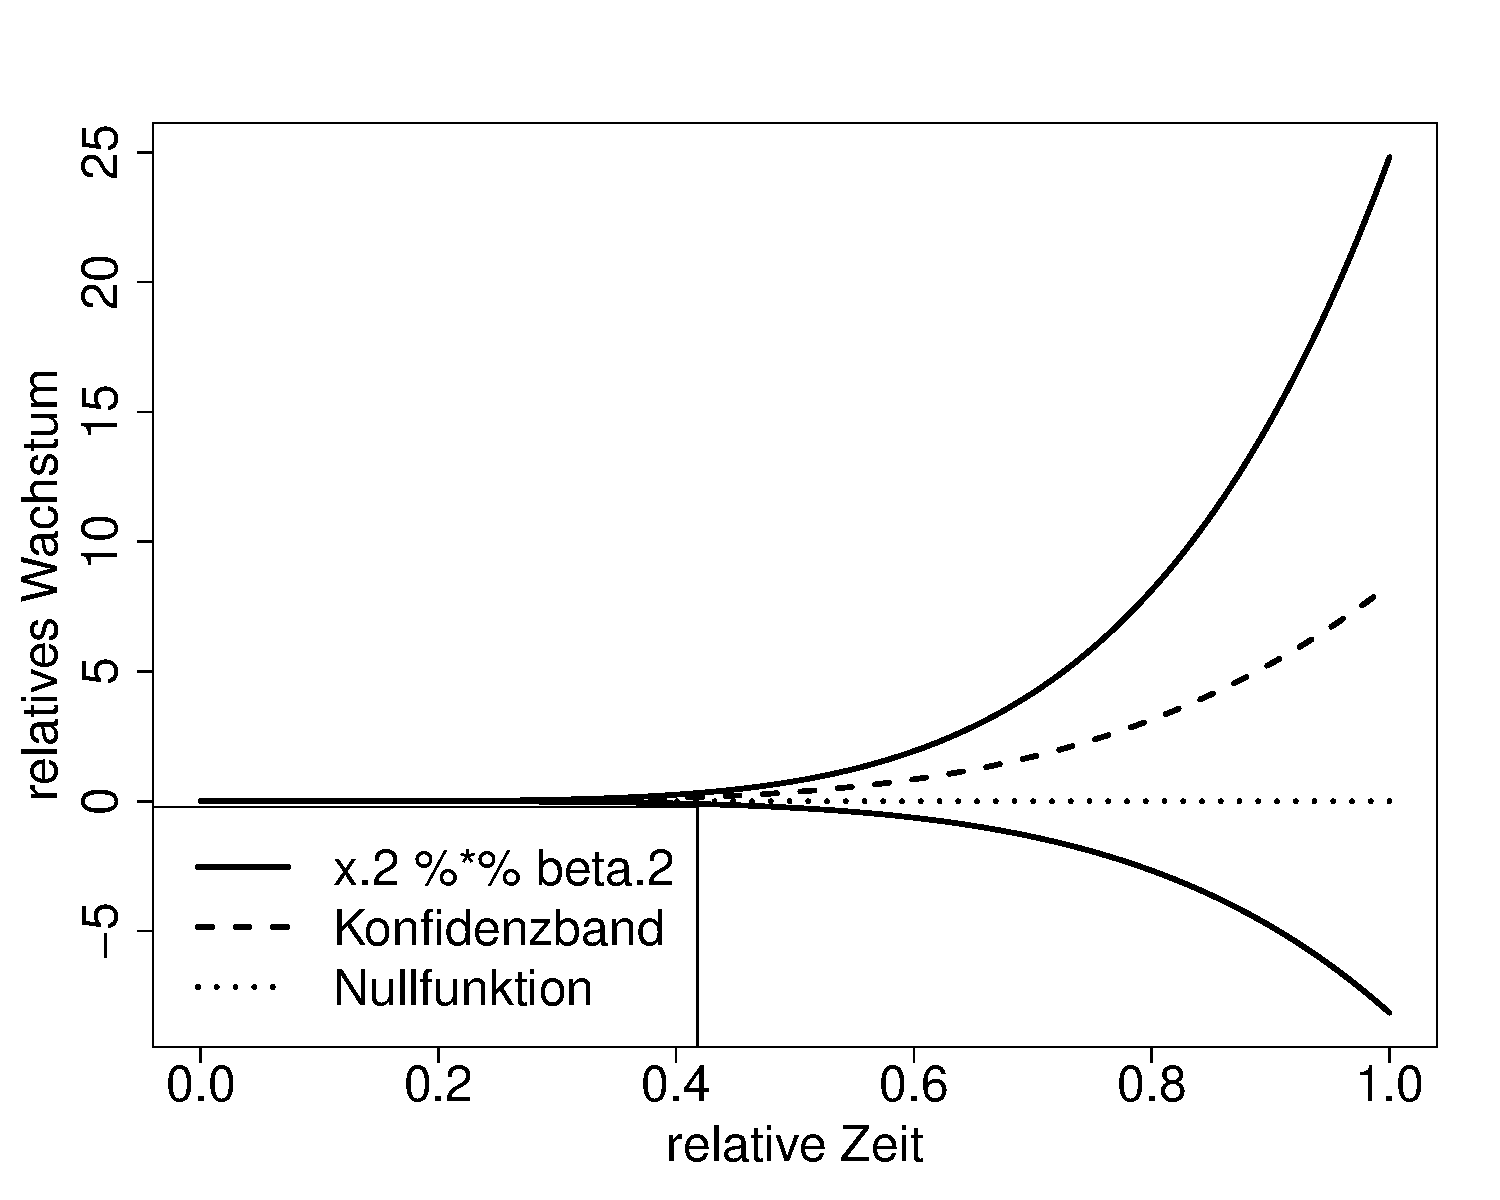
\includegraphics[width=0.5\textwidth]{10kPa-Grad-6-2-KB}
  \caption{10kPa Grad 6.2}
  \label{10kPa Grad 6.2}
\end{figure}



\nocite{Hsu41}

\newpage
\printbibliography


\newpage
\subsection*{Selbstständigkeitserklärung}
\addcontentsline{toc}{section}{Selbstständigkeitserklärung}
Hiermit bestätige ich, dass ich die vorliegende Arbeit selbstständig, nur mit Hilfe meiner Betreuer und ohne Benutzung anderer als der angegebenen Hilfsmittel angefertigt habe. Die aus fremden Quellen (einschließlich elektronischer Quellen) direkt oder indirekt übernommenen Gedanken sind ausnahmslos als solche kenntlich gemacht. Die Arbeit ist in gleicher oder ähnlicher Form oder auszugsweise im Rahmen einer anderen Prüfung noch nicht vorgelegt worden.
\\ \\ \\ \\
\parbox{5cm}{\centering Göttingen, ... }
%\hrule \strut \centering\footnotesize Ort, Datum} 
\hfill\parbox{4cm}{\hrule \strut \centering  \footnotesize Henning Hause}
\end{document}